\documentclass[]{book}
\usepackage{lmodern}
\usepackage{amssymb,amsmath}
\usepackage{ifxetex,ifluatex}
\usepackage{fixltx2e} % provides \textsubscript
\ifnum 0\ifxetex 1\fi\ifluatex 1\fi=0 % if pdftex
  \usepackage[T1]{fontenc}
  \usepackage[utf8]{inputenc}
\else % if luatex or xelatex
  \ifxetex
    \usepackage{mathspec}
  \else
    \usepackage{fontspec}
  \fi
  \defaultfontfeatures{Ligatures=TeX,Scale=MatchLowercase}
\fi
% use upquote if available, for straight quotes in verbatim environments
\IfFileExists{upquote.sty}{\usepackage{upquote}}{}
% use microtype if available
\IfFileExists{microtype.sty}{%
\usepackage{microtype}
\UseMicrotypeSet[protrusion]{basicmath} % disable protrusion for tt fonts
}{}
\usepackage[margin=1in]{geometry}
\usepackage{hyperref}
\hypersetup{unicode=true,
            pdftitle={Computational Statistics - Summary},
            pdfauthor={Lorenz Walthert},
            pdfborder={0 0 0},
            breaklinks=true}
\urlstyle{same}  % don't use monospace font for urls
\usepackage{color}
\usepackage{fancyvrb}
\newcommand{\VerbBar}{|}
\newcommand{\VERB}{\Verb[commandchars=\\\{\}]}
\DefineVerbatimEnvironment{Highlighting}{Verbatim}{commandchars=\\\{\}}
% Add ',fontsize=\small' for more characters per line
\usepackage{framed}
\definecolor{shadecolor}{RGB}{248,248,248}
\newenvironment{Shaded}{\begin{snugshade}}{\end{snugshade}}
\newcommand{\KeywordTok}[1]{\textcolor[rgb]{0.13,0.29,0.53}{\textbf{{#1}}}}
\newcommand{\DataTypeTok}[1]{\textcolor[rgb]{0.13,0.29,0.53}{{#1}}}
\newcommand{\DecValTok}[1]{\textcolor[rgb]{0.00,0.00,0.81}{{#1}}}
\newcommand{\BaseNTok}[1]{\textcolor[rgb]{0.00,0.00,0.81}{{#1}}}
\newcommand{\FloatTok}[1]{\textcolor[rgb]{0.00,0.00,0.81}{{#1}}}
\newcommand{\ConstantTok}[1]{\textcolor[rgb]{0.00,0.00,0.00}{{#1}}}
\newcommand{\CharTok}[1]{\textcolor[rgb]{0.31,0.60,0.02}{{#1}}}
\newcommand{\SpecialCharTok}[1]{\textcolor[rgb]{0.00,0.00,0.00}{{#1}}}
\newcommand{\StringTok}[1]{\textcolor[rgb]{0.31,0.60,0.02}{{#1}}}
\newcommand{\VerbatimStringTok}[1]{\textcolor[rgb]{0.31,0.60,0.02}{{#1}}}
\newcommand{\SpecialStringTok}[1]{\textcolor[rgb]{0.31,0.60,0.02}{{#1}}}
\newcommand{\ImportTok}[1]{{#1}}
\newcommand{\CommentTok}[1]{\textcolor[rgb]{0.56,0.35,0.01}{\textit{{#1}}}}
\newcommand{\DocumentationTok}[1]{\textcolor[rgb]{0.56,0.35,0.01}{\textbf{\textit{{#1}}}}}
\newcommand{\AnnotationTok}[1]{\textcolor[rgb]{0.56,0.35,0.01}{\textbf{\textit{{#1}}}}}
\newcommand{\CommentVarTok}[1]{\textcolor[rgb]{0.56,0.35,0.01}{\textbf{\textit{{#1}}}}}
\newcommand{\OtherTok}[1]{\textcolor[rgb]{0.56,0.35,0.01}{{#1}}}
\newcommand{\FunctionTok}[1]{\textcolor[rgb]{0.00,0.00,0.00}{{#1}}}
\newcommand{\VariableTok}[1]{\textcolor[rgb]{0.00,0.00,0.00}{{#1}}}
\newcommand{\ControlFlowTok}[1]{\textcolor[rgb]{0.13,0.29,0.53}{\textbf{{#1}}}}
\newcommand{\OperatorTok}[1]{\textcolor[rgb]{0.81,0.36,0.00}{\textbf{{#1}}}}
\newcommand{\BuiltInTok}[1]{{#1}}
\newcommand{\ExtensionTok}[1]{{#1}}
\newcommand{\PreprocessorTok}[1]{\textcolor[rgb]{0.56,0.35,0.01}{\textit{{#1}}}}
\newcommand{\AttributeTok}[1]{\textcolor[rgb]{0.77,0.63,0.00}{{#1}}}
\newcommand{\RegionMarkerTok}[1]{{#1}}
\newcommand{\InformationTok}[1]{\textcolor[rgb]{0.56,0.35,0.01}{\textbf{\textit{{#1}}}}}
\newcommand{\WarningTok}[1]{\textcolor[rgb]{0.56,0.35,0.01}{\textbf{\textit{{#1}}}}}
\newcommand{\AlertTok}[1]{\textcolor[rgb]{0.94,0.16,0.16}{{#1}}}
\newcommand{\ErrorTok}[1]{\textcolor[rgb]{0.64,0.00,0.00}{\textbf{{#1}}}}
\newcommand{\NormalTok}[1]{{#1}}
\usepackage{longtable,booktabs}
\usepackage{graphicx,grffile}
\makeatletter
\def\maxwidth{\ifdim\Gin@nat@width>\linewidth\linewidth\else\Gin@nat@width\fi}
\def\maxheight{\ifdim\Gin@nat@height>\textheight\textheight\else\Gin@nat@height\fi}
\makeatother
% Scale images if necessary, so that they will not overflow the page
% margins by default, and it is still possible to overwrite the defaults
% using explicit options in \includegraphics[width, height, ...]{}
\setkeys{Gin}{width=\maxwidth,height=\maxheight,keepaspectratio}
\IfFileExists{parskip.sty}{%
\usepackage{parskip}
}{% else
\setlength{\parindent}{0pt}
\setlength{\parskip}{6pt plus 2pt minus 1pt}
}
\setlength{\emergencystretch}{3em}  % prevent overfull lines
\providecommand{\tightlist}{%
  \setlength{\itemsep}{0pt}\setlength{\parskip}{0pt}}
\setcounter{secnumdepth}{5}
% Redefines (sub)paragraphs to behave more like sections
\ifx\paragraph\undefined\else
\let\oldparagraph\paragraph
\renewcommand{\paragraph}[1]{\oldparagraph{#1}\mbox{}}
\fi
\ifx\subparagraph\undefined\else
\let\oldsubparagraph\subparagraph
\renewcommand{\subparagraph}[1]{\oldsubparagraph{#1}\mbox{}}
\fi

%%% Use protect on footnotes to avoid problems with footnotes in titles
\let\rmarkdownfootnote\footnote%
\def\footnote{\protect\rmarkdownfootnote}

%%% Change title format to be more compact
\usepackage{titling}

% Create subtitle command for use in maketitle
\newcommand{\subtitle}[1]{
  \posttitle{
    \begin{center}\large#1\end{center}
    }
}

\setlength{\droptitle}{-2em}
  \title{Computational Statistics - Summary}
  \pretitle{\vspace{\droptitle}\centering\huge}
  \posttitle{\par}
  \author{Lorenz Walthert}
  \preauthor{\centering\large\emph}
  \postauthor{\par}
  \date{}
  \predate{}\postdate{}


\begin{document}
\maketitle

{
\setcounter{tocdepth}{1}
\tableofcontents
}
\chapter{Introduction}\label{introduction}

This is a summary (or rather rephrased version) of the class
computational statistics at ETH Zurich, enriched with notes from the
lecture, examples and R code. The main source is the
\href{https://polybox.ethz.ch/index.php/s/q3NaRdR7K6Xrfkd/download}{script}
of the course.

\chapter{Multiple Linear Regression}\label{multiple-linear-regression}

\chapter{Non-parametric Density
Estimation}\label{non-parametric-density-estimation}

We assume a model of the form

\[ E[Y|X = x] = m(x)\] which is more general than assuming
\(Y_i = m(x_i) + \epsilon_i\) since in the former, the noise does not
have to be additive. We can use Bayes' Theorem to deduce such an
estimator \(\hat{m}\) using density estimates of our predictor and
response variable. In that sense, non-parametric regression really
builds on top of non-parametric density estimation.

\begin{equation}
\begin{split}
P[Y|X] &=  \frac{\mathbb{P}[X|Y]}{\mathbb{P}[Y]}\mathbb{P}[Y] \\ 
f_{Y|X} & = \frac{f_{X|Y}}{f_X}f_Y \\
f_{Y|X} & = \frac{f_{X, Y}}{f_X}   \;\;\;\;\;\;\;\;\;\;\;\;\;\;\;\;\;\;\;\;\; \text{|} \times y\\
f_{Y|X}y & = \frac{f_{X, Y}}{f_X}y \;\;\;\;\;\;\;\;\;\;\;\;\;\;\;\;\;\;\;\; \text{| taking the integral}\\
E[X|Y] & = \int \frac{f_{X, Y}}{f_X}ydy
\end{split}
\end{equation}

Whereas for \(\hat{f}_{X, Y}\), we can use a product kernel. This
formula simplifies quite a bit and yields the Nadaraja-Watson Kernel,
which is essentially just a weighted mean of response values.
\[\hat{m}(x) = \frac{\sum\limits_{i = 1}^n K\Big(\frac{x-X_i}{h}\Big)Y_i}{\sum\limits_{i = 1}^nK\Big(\frac{x-X_i}{h}\Big)} = \frac{\sum\mathcal{w}_i Y_i}{\sum\mathcal{w}_i} = \sum\limits_{i = 1}^n \tilde{\mathcal{w}}_i Y_i = \tilde{\mathbf{w}}(x_i)'\mathbf{Y}\]
The weights \(\tilde{\mathcal{w}}_i\) are normalized weights, i.e.
\(\tilde{\mathcal{w}}_i = \mathcal{w}_i / \sum\limits_{k = 1}^n \mathcal{w}_k\)

\section{Alternative Interpretation}\label{alternative-interpretation}

It can be easily shown that the solution corresponds to the following
minimization problem:

\[ m(x) = \arg\min\limits_{m_x} \sum\limits_{i = 1}^nK\Big(\frac{x-X_i}{h}\Big)\big(Y_i-m_x\big)^2 \]

We can interpret this as a weighted (local) regression. For a given
\(x\), search for the best local constant \(m_x\) that minimizes the
weighted residual sum of squares the most. Residuals of data points
close to \(x\) get a high weight in this sum (via the kernel).

\section{The Bandwidth}\label{the-bandwidth}

The bandwidth parameter \(h\) has a similar role as in non-parametric
density estimation. Large \(h\) implies very smooth functions, low
variance, high bias. Small \(h\) on the other hand imply (more) erratic
functions, high variance, low bias.

An interesting case is \(h \rightarrow \infty\), for which all weights
become equal. This corresponds to an estimator \(m(x) = \bar{y}\), with
one degree of freedom (see below).

\section{Hat Matrix}\label{hat-matrix}

As in chapter 1, we can also obtain a smoother matrix \(S\) that maps
the observed response values to the fitted values. From above, we have:
\[\hat{y}_i = \tilde{\mathbf{w}}(x_i)'\mathbf{Y}\]

\[\mathbf{\hat{Y}} = \mathcal{S} \mathbf{Y} = 
\begin{pmatrix}\hat{y}_1 \\\vdots\\\hat{y}_n\end{pmatrix} =
\begin{pmatrix}\tilde{\mathbf{w}}(x_1)'\\\vdots\\\tilde{\mathbf{w}}(x_n)'\end{pmatrix} 
\times \begin{pmatrix}y_1 \\\vdots\\y_n\end{pmatrix}\] Where
\(\tilde{\mathbf{w}}(x_1)'\) is a row vector of length \(n\) with the
normalized kernel weights.

** here: How to compute S and why**

\section{Degrees of Freedom}\label{degrees-of-freedom}

Note that we need a different measurement of degrees of freedom than the
one we used in the \emph{parametric} case in chapter 1, where the
degrees of freedom simply corresponded to the number of parameters used.
As this is non-parametric regression, we don't have parameters and hence
cannot sum up the number of parameters to calculate the degree of
freedom. Recall from chapter 1 that the trace of the smoothing matrix
was equal to the number of parameters used:
\[tr(P) = \textbf{tr}(X(X'X)^{-1}X') = \textbf{tr}((X'X)^{-1}X'X) = \textbf{tr}(I_{p\times p}) = p\]
Hence, we can generalize the concept of degrees of freedom from number
of parameters to the trace of the smoother matrix. For regression, the
two coincide, for non-parametric methods, we get an estimate of the
degrees of freedom only via the trace.

There is a one-to-one relationship between the degrees of freedom and
the bandwidth parameter \(h\), which we can show in a diagram:

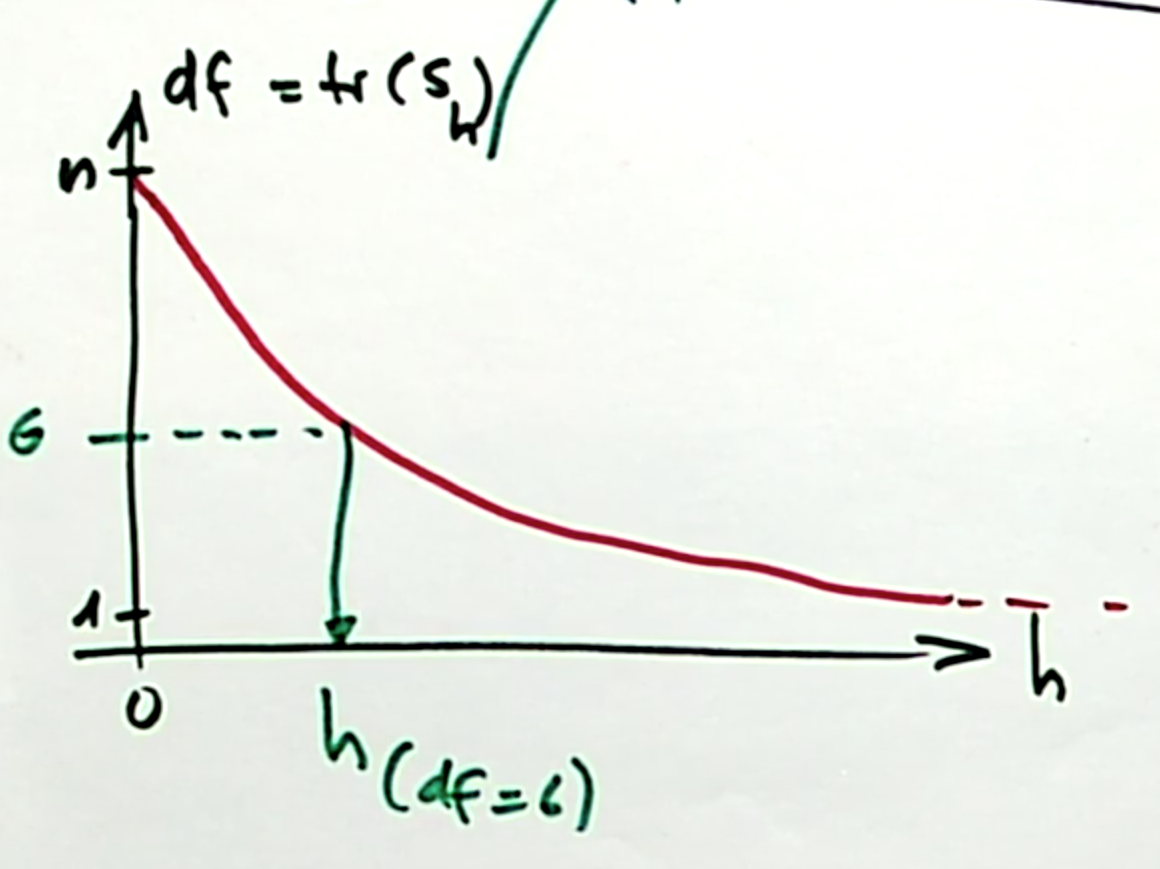
\includegraphics[width=650px]{figures/relationship-h-df}

This can be derived from the two extreme cases:

\begin{itemize}
\tightlist
\item
  \(h \rightarrow \infty\) means all weights are equal, which means for
  each data point \(x_i\), the fitted value \(\hat{m}(x_i)\) is just the
  grand mean of \(y\). This corresponds to one degree of freedom.
\end{itemize}

\[\hat{m}(x) = \bar{y} \]

\begin{itemize}
\tightlist
\item
  \(h \rightarrow 0\). If we assume \(n\) distinct, equi-spaced \(x_i\)
  values, then the fitted values in the neighborhood of \(\hat{m}(x_i)\)
  are just the observed response value \(y_i\), since all weights for
  points other than \(y_i\) are zero. Or to be more precise: If the
  distance between neighboring points is \(\eta\), then, for
  \(h \leqslant \eta\) :
  \[ \hat{m}(x) = y_{i^*} \;\;\ \text{with} \;\; i^* =  
    \arg\min\limits_{0 \leqslant i \leqslant n} |x - x_i| \] This
  corresponds to \(n\) degrees of freedom.
\item
  We can interpolate between these two extreme cases in a monotone way.
\end{itemize}

\subsection{Applications}\label{applications}

There are two main applications for the degree of freedom:

\begin{itemize}
\tightlist
\item
  \textbf{As a tuning parameter}. For every \(h\), we can find the
  corresponding degrees of freedom or more interestingly - for
  every(desired) degree of freedom, we can find an \(h\). Instead of
  varying \(h\) directly, we can vary the degrees of freedom, which are
  directly \textbf{comparable} accross different techniques. We can
  compare OLS with different kernel smoothers, splines etc. (see below),
  which is not possible with \(h\) alone.
\item
  \textbf{For inference}. For unbiased estimators (such as the variance
  of the residuals), we need the degrees of freedom (see below).
\end{itemize}

\section{Inference}\label{inference}

As with parametric regression, we want to do inference. Not on any
parameters (since there are none), but on the fitted values. First and
foremost, we want to obtain confidence intervals for the regression
line, that is, obtaining point-wise lower and upper bounds of the
confidence internal
\[ I_i = \hat{m}(x_i) ± 1.96 *\hat{sd}(\hat{m}(x)) \] Which holds
because the fitted value is asymtotically normally distributed. We know
already how to obtain \(\hat{m}(x)\), now we need to find the standard
deviation of the fitted values.

From the fundamental equation
\(Cov(\mathbf{A}x) = \mathbf{A} Cov(x) \mathbf{A}'\), we get
\[ \text{Cov}(\hat{m}(x)) = \text{Cov}(\mathcal{S}\mathbf{y}) = 
\mathcal{S} \text{Cov}(y) \mathcal{S}' = \sigma_\epsilon^2\mathcal{SS}'
\;\;\;\;\;|\;\; \text{since Cov}(y) = \text{Cov}(\epsilon)\] Which is a
\(p\times p\) matrix. For a specific data point \(x_i\), we have
\[ \text{Var}(\hat{m}(x_i))= \text{Cov}(\hat{m}(x_i),  \hat{m}(x_i)) = \sigma_\epsilon^2 (\mathcal{S} \mathcal{S}')_{ii} \]

Now, we only need to estimate \(\sigma^2_\epsilon\). Using the
generalized method to compute degrees of freedom, we can use the
following estimator:

\[ \hat{\sigma}_\epsilon^2 = \frac{1}{n-\textbf{tr}(\mathcal{S})} 
\sum\limits_{i = 1}^n (Y_i - \hat{m}(x_i))^2 \]

\section{Local Polynomial Estimator}\label{local-polynomial-estimator}

Expanding on the formulation of the Nadaraya-Watson Kernel as a weighted
least square problem, we can use centered polynomials to approximate
\(y_i\) instead of a local constant \(\hat{m}_x\). That is, computing
our estimator as

\[\hat{m}(x) = \arg\min\limits_{m_x} \sum\limits_{i = 1}^nK\Big(\frac{x-X_i}{h}\Big)
\big(Y_i-\beta_0 + \beta_1 (x_i -x) + ... \beta_{p-1} (x_i-x)^{p-1}\big)^2 \]

This has the advantage of yielding a \emph{lolcal linear} regression
curve at the borders, whereas the Nadaraya-Watson Kernel yields
\emph{local constant} regression curves in these regions (since at the
border, no new points are are taken into account).

Another advantage is that we can find derivaties of the regression
estimate at each point easily.

\chapter{Non-parametric Regression}\label{non-parametric-regression}

We assume a model of the form

\[ E[Y|X = x] = m(x)\] which is more general than assuming
\(Y_i = m(x_i) + \epsilon_i\) since in the former, the noise does not
have to be additive. We can use Bayes' Theorem to deduce such an
estimator \(\hat{m}\) using density estimates of our predictor and
response variable. In that sense, non-parametric regression really
builds on top of non-parametric density estimation.

\begin{equation}
\begin{split}
P[Y|X] &=  \frac{\mathbb{P}[X|Y]}{\mathbb{P}[Y]}\mathbb{P}[Y] \\ 
f_{Y|X} & = \frac{f_{X|Y}}{f_X}f_Y \\
f_{Y|X} & = \frac{f_{X, Y}}{f_X}   \;\;\;\;\;\;\;\;\;\;\;\;\;\;\;\;\;\;\;\;\; \text{|} \times y\\
f_{Y|X}y & = \frac{f_{X, Y}}{f_X}y \;\;\;\;\;\;\;\;\;\;\;\;\;\;\;\;\;\;\;\; \text{| taking the integral}\\
E[X|Y] & = \int \frac{f_{X, Y}}{f_X}ydy
\end{split}
\end{equation}

Whereas for \(\hat{f}_{X, Y}\), we can use a product kernel. This
formula simplifies quite a bit and yields the Nadaraja-Watson Kernel,
which is essentially just a weighted mean of response values.
\[\hat{m}(x) = \frac{\sum\limits_{i = 1}^n K\Big(\frac{x-X_i}{h}\Big)Y_i}{\sum\limits_{i = 1}^nK\Big(\frac{x-X_i}{h}\Big)} = \frac{\sum\mathcal{w}_i Y_i}{\sum\mathcal{w}_i} = \sum\limits_{i = 1}^n \tilde{\mathcal{w}}_i Y_i = \tilde{\mathbf{w}}(x_i)'\mathbf{Y}\]
The weights \(\tilde{\mathcal{w}}_i\) are normalized weights, i.e.
\(\tilde{\mathcal{w}}_i = \mathcal{w}_i / \sum\limits_{k = 1}^n \mathcal{w}_k\)

\section{Alternative Interpretation}\label{alternative-interpretation-1}

It can be easily shown that the solution corresponds to the following
minimization problem:

\[ m(x) = \arg\min\limits_{m_x} \sum\limits_{i = 1}^nK\Big(\frac{x-X_i}{h}\Big)\big(Y_i-m_x\big)^2 \]

We can interpret this as a weighted (local) regression. For a given
\(x\), search for the best local constant \(m_x\) that minimizes the
weighted residual sum of squares the most. Residuals of data points
close to \(x\) get a high weight in this sum (via the kernel).

\section{The Bandwidth}\label{the-bandwidth-1}

The bandwidth parameter \(h\) has a similar role as in non-parametric
density estimation. Large \(h\) implies very smooth functions, low
variance, high bias. Small \(h\) on the other hand imply (more) erratic
functions, high variance, low bias.

An interesting case is \(h \rightarrow \infty\), for which all weights
become equal. This corresponds to an estimator \(m(x) = \bar{y}\), with
one degree of freedom (see below).

\section{Hat Matrix}\label{hat-matrix-1}

As in chapter 1, we can also obtain a smoother matrix \(S\) that maps
the observed response values to the fitted values. From above, we have:
\[\hat{y}_i = \tilde{\mathbf{w}}(x_i)'\mathbf{Y}\]

\[\mathbf{\hat{Y}} = \mathcal{S} \mathbf{Y} = 
\begin{pmatrix}\hat{y}_1 \\\vdots\\\hat{y}_n\end{pmatrix} =
\begin{pmatrix}\tilde{\mathbf{w}}(x_1)'\\\vdots\\\tilde{\mathbf{w}}(x_n)'\end{pmatrix} 
\times \begin{pmatrix}y_1 \\\vdots\\y_n\end{pmatrix}\] Where
\(\tilde{\mathbf{w}}(x_1)'\) is a row vector of length \(n\) with the
normalized kernel weights.

** here: How to compute S and why**

\section{Degrees of Freedom}\label{degrees-of-freedom-1}

Note that we need a different measurement of degrees of freedom than the
one we used in the \emph{parametric} case in chapter 1, where the
degrees of freedom simply corresponded to the number of parameters used.
As this is non-parametric regression, we don't have parameters and hence
cannot sum up the number of parameters to calculate the degree of
freedom. Recall from chapter 1 that the trace of the smoothing matrix
was equal to the number of parameters used:
\[tr(P) = \textbf{tr}(X(X'X)^{-1}X') = \textbf{tr}((X'X)^{-1}X'X) = \textbf{tr}(I_{p\times p}) = p\]
Hence, we can generalize the concept of degrees of freedom from number
of parameters to the trace of the smoother matrix. For regression, the
two coincide, for non-parametric methods, we get an estimate of the
degrees of freedom only via the trace.

There is a one-to-one relationship between the degrees of freedom and
the bandwidth parameter \(h\), which we can show in a diagram:

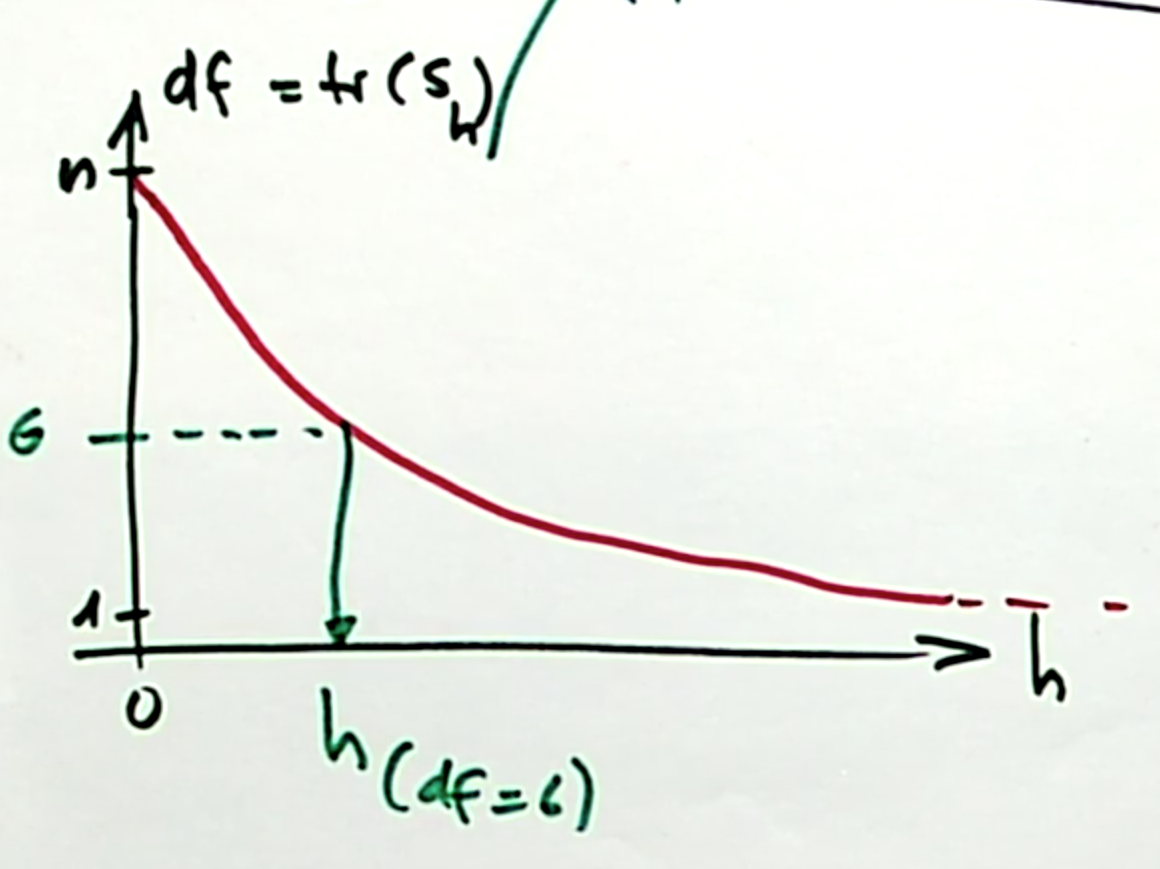
\includegraphics[width=650px]{figures/relationship-h-df}

This can be derived from the two extreme cases:

\begin{itemize}
\tightlist
\item
  \(h \rightarrow \infty\) means all weights are equal, which means for
  each data point \(x_i\), the fitted value \(\hat{m}(x_i)\) is just the
  grand mean of \(y\). This corresponds to one degree of freedom.
\end{itemize}

\[\hat{m}(x) = \bar{y} \]

\begin{itemize}
\tightlist
\item
  \(h \rightarrow 0\). If we assume \(n\) distinct, equi-spaced \(x_i\)
  values, then the fitted values in the neighborhood of \(\hat{m}(x_i)\)
  are just the observed response value \(y_i\), since all weights for
  points other than \(y_i\) are zero. Or to be more precise: If the
  distance between neighboring points is \(\eta\), then, for
  \(h \leqslant \eta\) :
  \[ \hat{m}(x) = y_{i^*} \;\;\ \text{with} \;\; i^* =  
    \arg\min\limits_{0 \leqslant i \leqslant n} |x - x_i| \] This
  corresponds to \(n\) degrees of freedom.
\item
  We can interpolate between these two extreme cases in a monotone way.
\end{itemize}

\subsection{Applications}\label{applications-1}

There are two main applications for the degree of freedom:

\begin{itemize}
\tightlist
\item
  \textbf{As a tuning parameter}. For every \(h\), we can find the
  corresponding degrees of freedom or more interestingly - for
  every(desired) degree of freedom, we can find an \(h\). Instead of
  varying \(h\) directly, we can vary the degrees of freedom, which are
  directly \textbf{comparable} accross different techniques. We can
  compare OLS with different kernel smoothers, splines etc. (see below),
  which is not possible with \(h\) alone.
\item
  \textbf{For inference}. For unbiased estimators (such as the variance
  of the residuals), we need the degrees of freedom (see below).
\end{itemize}

\section{Inference}\label{inference-1}

As with parametric regression, we want to do inference. Not on any
parameters (since there are none), but on the fitted values. First and
foremost, we want to obtain confidence intervals for the regression
line, that is, obtaining point-wise lower and upper bounds of the
confidence internal
\[ I_i = \hat{m}(x_i) ± 1.96 *\hat{sd}(\hat{m}(x)) \] Which holds
because the fitted value is asymtotically normally distributed. We know
already how to obtain \(\hat{m}(x)\), now we need to find the standard
deviation of the fitted values.

From the fundamental equation
\(Cov(\mathbf{A}x) = \mathbf{A} Cov(x) \mathbf{A}'\), we get
\[ \text{Cov}(\hat{m}(x)) = \text{Cov}(\mathcal{S}\mathbf{y}) = 
\mathcal{S} \text{Cov}(y) \mathcal{S}' = \sigma_\epsilon^2\mathcal{SS}'
\;\;\;\;\;|\;\; \text{since Cov}(y) = \text{Cov}(\epsilon)\] Which is a
\(p\times p\) matrix. For a specific data point \(x_i\), we have
\[ \text{Var}(\hat{m}(x_i))= \text{Cov}(\hat{m}(x_i),  \hat{m}(x_i)) = \sigma_\epsilon^2 (\mathcal{S} \mathcal{S}')_{ii} \]

Now, we only need to estimate \(\sigma^2_\epsilon\). Using the
generalized method to compute degrees of freedom, we can use the
following estimator:

\[ \hat{\sigma}_\epsilon^2 = \frac{1}{n-\textbf{tr}(\mathcal{S})}
\sum\limits_{i = 1}^n (Y_i - \hat{m}(x_i))^2\]

\section{Local Polynomial Estimator}\label{local-polynomial-estimator-1}

Expanding on the formulation of the Nadaraya-Watson Kernel as a weighted
least square problem, we can use centered polynomials to approximate
\(y_i\) instead of a local constant \(\hat{m}_x\). That is, computing
our estimator as

\[\hat{m}(x) = \arg\min\limits_{m_x} \sum\limits_{i = 1}^nK\Big(\frac{x-X_i}{h}\Big)
\big(Y_i-\beta_0 + \beta_1 (x_i -x) + ... \beta_{p-1} (x_i-x)^{p-1}\big)^2 \]

This has the advantage of yielding a \emph{lolcal linear} regression
curve at the borders, whereas the Nadaraya-Watson Kernel yields
\emph{local constant} regression curves in these regions (since at the
border, no new points are are taken into account).

Another advantage is that we can find derivaties of the regression
estimate at each point easily.

\chapter{Cross Validation}\label{cross-validation}

\section{Motivation and Core Idea}\label{motivation-and-core-idea}

Cross-validation is a tool for estimating the performance of an
algorithm on new data points, the so-called the generalization error. An
estimate of the generalization allows us to do two important things:

\begin{itemize}
\tightlist
\item
  Tuning the parameters of a statistical technique.
\item
  Comparing statistical techniques with regard to their accuracy.
\end{itemize}

If we use the \textbf{training data} to evaluate the performance of an
algorithm, this estimate will be over-optimistic because an estimator is
usually obtained by minimizing some sort of error in the training data.
Therefore, we use a separate data pool, called the \textbf{test data} to
evaluate the performance out of sample. Consider the regression function
estimate \(\hat{m}\) based on a sample \((X_1, ..., X_n.)\). By
increasing the number of parameters in the model and by allowing for
interactions between them, we can make the regression model fitting
arbitrarily well to the data. However, such an extremely complex model
will not perform as well with new data, that is, will not generalize
well to other data sets, since we essentially modeled also a lot of
noise. To estimate the performance of an algorithm on a new sample, we
introduce the following notation:
\[ l^{-1}\sum\limits_{i = 1}^l\rho(Y_{new, i}, \hat{g}(X_{new, i}))\]
Where \(\rho\) is a loss function to be evaluated on the new data points
\((Y_{new, 1}, ..., Y_{new, l})\) and the prediction made for
\((X_{new, 1}, ..., X_{new, l})\) with the function \(\hat{g}\), which
was estimated from the training data \((X_1, ..., X_n)\). When \(l\)
gets large, this approximates the \textbf{test error}
\[\mathbb{E}_{(X_{new}, Y_{new})}[\rho(Y_{new}, \hat{m}(X_{new})]\]
which is still a function of the training data (since it is conditional
on the training data). Note that the \emph{test error} is not the same
as the \textbf{generalization error}. The latter is an expectation over
both the training and the test data. The typical relationship between
the test error and the training error is depicted in the figure below.

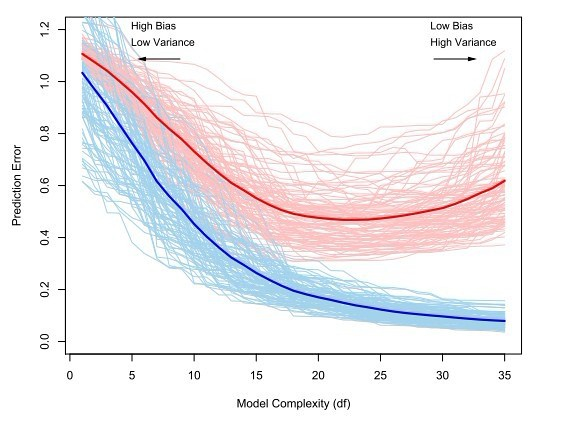
\includegraphics[width=650px]{figures/ge}

The optimal model complexity is at around \(20\) degrees of freedom.
With more degrees of freedom, the test set error increases again. We
start to model noise. This is also called overfitting.

\section{Loss Function}\label{loss-function}

Depending on the application, one can imagine different loss-functions.
For example the squared deviance from the \emph{true} value is often
used, i.e.
\[n^{-1}\sum\limits_{i = 1}^n\rho(Y_i, \hat{m}(X_i)) = n^{-1}\sum\limits_{i = 1}^n(Y_i - \hat{m}(X_i))^2\]
Hence, larger deviance is penalized over-proportionally. For
classification, one often uses the zero-one error, i.e.
\[n^{-1}\sum\limits_{i = 1}^n1_{\hat{m}(X_i) \neq Y_i}\] However, it
might also be appropriate to use asymmetric loss functions if false
negatives are worse than false positives (i.e.~for cancer tests).

\section{Implementation}\label{implementation}

There are different ways to do cross validation while adhering to the
principles introduced above.

\subsection{Leave-one-out}\label{leave-one-out}

\begin{itemize}
\tightlist
\item
  Use all but one data point to construct a model and predict on the
  remaining data point.
\item
  Do that \(n\) times until all \(n\) points were used for prediction
  once.
\item
  Compute the test error as an average over all n errors measured, i.e
\end{itemize}

\[n^{-1}\sum\limits_{i = 1}^n \rho{(Y_{i}, \hat{m}_{n-1}^{-i}(X_i)})\]
And use that as an approximation of the \emph{generalization error}.

\section{K-fold Cross-Validation}\label{k-fold-cross-validation}

This method is best explained with a picture.

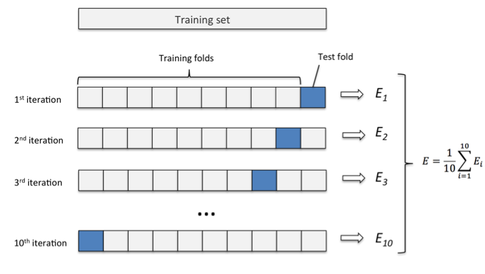
\includegraphics[width=650px]{figures/k_fold_cv}

Here, one splits the data set into k equally (or as equal as possible)
sized folds. Then, the idea is to use all \(k-1\) folds to build a model
and the remaining fold to evaluate the model. Then, we average the \(k\)
estimates of the generalization error. Or in mathematical notation:

\[K^{-1} \sum\limits_{k = 1}^K |B_k|^{-1} \sum\limits_{i \in B_k}\rho({Y_{i}, \hat{m}^{-B_k}_{n-|B_k|}(X_i))}\]

Note that leave-one out cv is the same as k-fold cross validation with
\(=n\).

\subsection{Random Division into test and training data
set}\label{random-division-into-test-and-training-data-set}

The problem of K-fold cross-validation is that it depends on \textbf{one
realization} of the split into k folds. Instead, we can generalize
leave-one-out to leave-d-out. That means, we remove \(d\) observations
from our initial data, apply our estimation procedure and evaluate on
the \(d\) observations.
\[\hat{\theta}^{-C_k}_{n-k} \;\;\; \text{for all possible subsets}\;\; C_k, \;\; k=1, ..., {\binom{n}{d}}\]
The generalization error can be estimated with
\[{\binom{n}{d}}^{-1}\sum\limits_{k = 1}^{\binom{n}{d}} d^{-1}\sum\limits_{i \in C_k} \rho(Y_i, \hat{m}^{-C_k}_{n-d}(X_i))\]
For \(d > 3\), the computational burden becomes immense. For that
reason, instead of considering all \({\binom{n}{d}}\) sets, we can
uniformly draw \(B\) sets (\(C_1^*, ... C_B^*\)) from
\(C_1, ..., C_{\binom{n}{d}}\) \emph{without replacement}. For
\(B=\binom{n}{d}\), we obviously get the full leave-d-out solution. The
\textbf{computational cost} for computing such an approximation to the
leave-d-out is linear in \(B\) (since evaluating is almost for free).
For leave-one-out, the cost is linear in \(n\) in the same way. Hence,
the stochastic approximation for leave-d-out can be even smaller than
for leave-one-out if \(B < n\).

\section{Properties of the different
schemes}\label{properties-of-the-different-schemes}

We can try to say something about both bias and variance of the cv
schemes introduced above.

\begin{itemize}
\tightlist
\item
  \textbf{leave-one-out} is an asymptotically \textbf{unbiased}
  estimator for the generalization error and the true prediction.
  However, we use a sample size \(n-1\) instead of \(n\), which causes a
  slight bias (meaning we have less data as we do in a real world
  scenario, which most likely makes the CV score a tiny little bit worse
  than it should be). Because the training sets are very similar to each
  other the leave-one-out scheme has a \textbf{large variance}.
\item
  \textbf{leave-d-out} has a \textbf{higher bias} than leave-one-out
  because the sample size is even smaller than \(n-1\) (for \(d>1\)).
  However, since we aggregate over more (\(\binom{n}{d}\) instead of
  \(n\)) cv scores, which can be shown to decrease the variance of the
  final cv estimator.
\item
  \textbf{k-fold} cv has a \textbf{higher bias} than both leave one out.
\end{itemize}

\section{Shortcuts for (some) linear fitting
operators}\label{shortcuts-for-some-linear-fitting-operators}

Leave-one-out cv score for some linear fitting procedures such as least
squares or smoothing spline can be computed via a shortcut when our loss
function is \(\rho(y, \hat{y}) = |y-\hat{y}|^2\). In particular, we can
compute the estimator for such a linear fitting procedure \textbf{once},
compute the linear fitting operator \(S\), which satisfies
\(\mathbf{\hat{Y}} = \mathbf{SY}\) and plug it in this formula:
\[n^{-1}\sum\limits_{i = 1}^n \Bigg(\frac{Y_i - \hat{m}(X_i)}{1-S_{ii}}\Bigg)^2\]
Computing \(\mathbf{S}\) requires \(O(n)\) operations (see exercises).

Historically, it has been computationally easier to compute the trace of
\(\mathbf{S}\) so there is also a quantity called generalized cross
validation (which is a misleading terminology), which coincides with the
formula above in certain cases.

\section{Examples}\label{examples}

\subsection{Practical CV in R}\label{practical-cv-in-r}

Key concepts to do CV are

\begin{itemize}
\tightlist
\item
  Do not split the data, split the indices of the data and work with
  them if ever possible and subset the data. \texttt{sample()} is your
  friend.
\item
  use \texttt{purrr::map()}, \texttt{purrr::map\_df()} and friends to
  ``loop'' over data. This is preferred over base R \texttt{lapply} /
  \texttt{mapply} / \texttt{Map} since it has a more coherent argument
  structure (consistent argument positioning, no strange
  \texttt{MoreArgs} arguments, pipable etc.)
\item
  you can simplify structures with \texttt{purr::flatten\_dbl()} and
  friends.
\item
  Always work with lists, never work with data frames of indices. The
  reason is that data frames have structural constrains (all columns
  must have same number of elements) that are not natural in some
  situations. For example, out-of-bootstrap cv \emph{does} have the same
  number of observations in the training set, but not in the test set.
\item
  In conjunction with \texttt{sample()}, you can use
  \texttt{purrr::rerun} or \texttt{replicate} to create lists of
  indices.
\item
  use helper function to solve ``the small problems in the big
  problem''.
\end{itemize}

Let's first declare our functions.

\begin{Shaded}
\begin{Highlighting}[]
\KeywordTok{library}\NormalTok{(}\StringTok{"purrr"}\NormalTok{)}
\KeywordTok{data}\NormalTok{(ozone, }\DataTypeTok{package =} \StringTok{"gss"}\NormalTok{)}

\CommentTok{#' Estimate the generalization error of a ridge regression}
\CommentTok{#' @param test Test indices.}
\CommentTok{#' @param train Train indices.}
\CommentTok{#' @param .data The data.}
\CommentTok{#' @param lamda The lamda parameter for the ridge regression.}
\NormalTok{ge_ridge <-}\StringTok{ }\NormalTok{function(test, train, .data, lambda) \{}
  \NormalTok{fit <-}\StringTok{ }\NormalTok{MASS::}\KeywordTok{lm.ridge}\NormalTok{(upo3~., }
                  \DataTypeTok{lambda =} \NormalTok{lambda,}
                  \DataTypeTok{data =} \NormalTok{.data[train,])}
  \NormalTok{pred <-}\StringTok{ }\KeywordTok{as.matrix}\NormalTok{(}\KeywordTok{cbind}\NormalTok{(}\DecValTok{1}\NormalTok{, .data[test, -}\DecValTok{1}\NormalTok{])) %*%}\StringTok{ }\KeywordTok{coef}\NormalTok{(fit)}
  \KeywordTok{mean}\NormalTok{((pred -}\StringTok{ }\NormalTok{.data[test,]$upo3)^}\DecValTok{2}\NormalTok{)}
\NormalTok{\}}


\NormalTok{##  ............................................................................}
\NormalTok{##  functions to return list with indices                                   ####}


\NormalTok{get_boostrap_mat <-}\StringTok{ }\NormalTok{function(B, n) \{}
  \KeywordTok{rerun}\NormalTok{(B, }\KeywordTok{sample}\NormalTok{(n, n, }\DataTypeTok{replace =} \OtherTok{TRUE}\NormalTok{))}
  
\NormalTok{\}}

\NormalTok{get_all_mat <-}\StringTok{ }\NormalTok{function(B, n) \{}
  \KeywordTok{rerun}\NormalTok{(B, }\DecValTok{1}\NormalTok{:n)}
\NormalTok{\}}

\NormalTok{get_complement <-}\StringTok{ }\NormalTok{function(mat, n)\{}
  \KeywordTok{map}\NormalTok{(mat, ~}\KeywordTok{setdiff}\NormalTok{(}\DecValTok{1}\NormalTok{:n, .x))}
\NormalTok{\}}

\NormalTok{get_k_fold_test <-}\StringTok{ }\NormalTok{function(k, n) \{}
  \NormalTok{step <-}\StringTok{ }\KeywordTok{trunc}\NormalTok{(n/k)}
  \NormalTok{current <-}\StringTok{ }\KeywordTok{list}\NormalTok{()}
  \NormalTok{for (i in (}\DecValTok{0}\NormalTok{:(k}\DecValTok{-1}\NormalTok{) *}\StringTok{ }\NormalTok{step +}\StringTok{ }\DecValTok{1}\NormalTok{))  \{}
    \NormalTok{current <-}\StringTok{ }\KeywordTok{append}\NormalTok{(}
      \NormalTok{current, }
      \KeywordTok{list}\NormalTok{(i:(i+step}\DecValTok{-1}\NormalTok{))}
    \NormalTok{)}
  \NormalTok{\}}
  \NormalTok{current}
\NormalTok{\}}
\end{Highlighting}
\end{Shaded}

Now, let us apply the functions for three cv schemes to estimate the
generalization error.

\begin{Shaded}
\begin{Highlighting}[]
\NormalTok{##  ............................................................................}
\NormalTok{##  boostrap                                                                ####}
\CommentTok{# use boostrap sample to train, use all to test}
\NormalTok{n <-}\StringTok{ }\KeywordTok{nrow}\NormalTok{(ozone)}
\NormalTok{train <-}\StringTok{ }\KeywordTok{get_boostrap_mat}\NormalTok{(}\DecValTok{10}\NormalTok{, n)}
\NormalTok{test <-}\StringTok{ }\KeywordTok{get_all_mat}\NormalTok{(}\DecValTok{10}\NormalTok{, n)}
\NormalTok{bs <-}\StringTok{ }\KeywordTok{map2_dbl}\NormalTok{(test, train, ge_ridge, }\DataTypeTok{.data =} \NormalTok{ozone, }\DataTypeTok{lambda =} \DecValTok{5}\NormalTok{)}



\NormalTok{##  ............................................................................}
\NormalTok{##  10-fold                                                                 ####}
\NormalTok{test <-}\StringTok{ }\KeywordTok{get_k_fold_test}\NormalTok{(}\DecValTok{10}\NormalTok{, n)}
\NormalTok{train <-}\StringTok{ }\KeywordTok{map}\NormalTok{(test, ~}\KeywordTok{setdiff}\NormalTok{(}\DecValTok{1}\NormalTok{:n, .x))}
\NormalTok{kfold <-}\StringTok{ }\KeywordTok{map2_dbl}\NormalTok{(test, train, ge_ridge, }\DataTypeTok{.data =} \NormalTok{ozone, }\DataTypeTok{lambda =} \DecValTok{5}\NormalTok{)}

\NormalTok{##  ............................................................................}
\NormalTok{##  out-of-boostrap                                                         ####}
\NormalTok{train <-}\StringTok{ }\KeywordTok{get_boostrap_mat}\NormalTok{(}\DecValTok{10}\NormalTok{, n)}
\NormalTok{test <-}\StringTok{ }\KeywordTok{map}\NormalTok{(test, ~}\KeywordTok{setdiff}\NormalTok{(}\DecValTok{1}\NormalTok{:n, .x))}
\NormalTok{oob <-}\StringTok{ }\KeywordTok{map2_dbl}\NormalTok{(test, train, ge_ridge, }\DataTypeTok{.data =} \NormalTok{ozone, }\DataTypeTok{lambda =} \DecValTok{5}\NormalTok{)}
\end{Highlighting}
\end{Shaded}

The results are as follows:

\begin{Shaded}
\begin{Highlighting}[]
\NormalTok{out <-}\StringTok{ }\KeywordTok{cbind}\NormalTok{(bs, kfold, oob) %>%}
\StringTok{  }\KeywordTok{as_data_frame}\NormalTok{() %>%}
\StringTok{  }\KeywordTok{gather}\NormalTok{(key, value)}

\KeywordTok{ggplot}\NormalTok{(out, }\KeywordTok{aes}\NormalTok{(}\DataTypeTok{y =} \NormalTok{value, }\DataTypeTok{x =} \NormalTok{key)) +}\StringTok{ }
\StringTok{  }\KeywordTok{geom_boxplot}\NormalTok{()}
\end{Highlighting}
\end{Shaded}

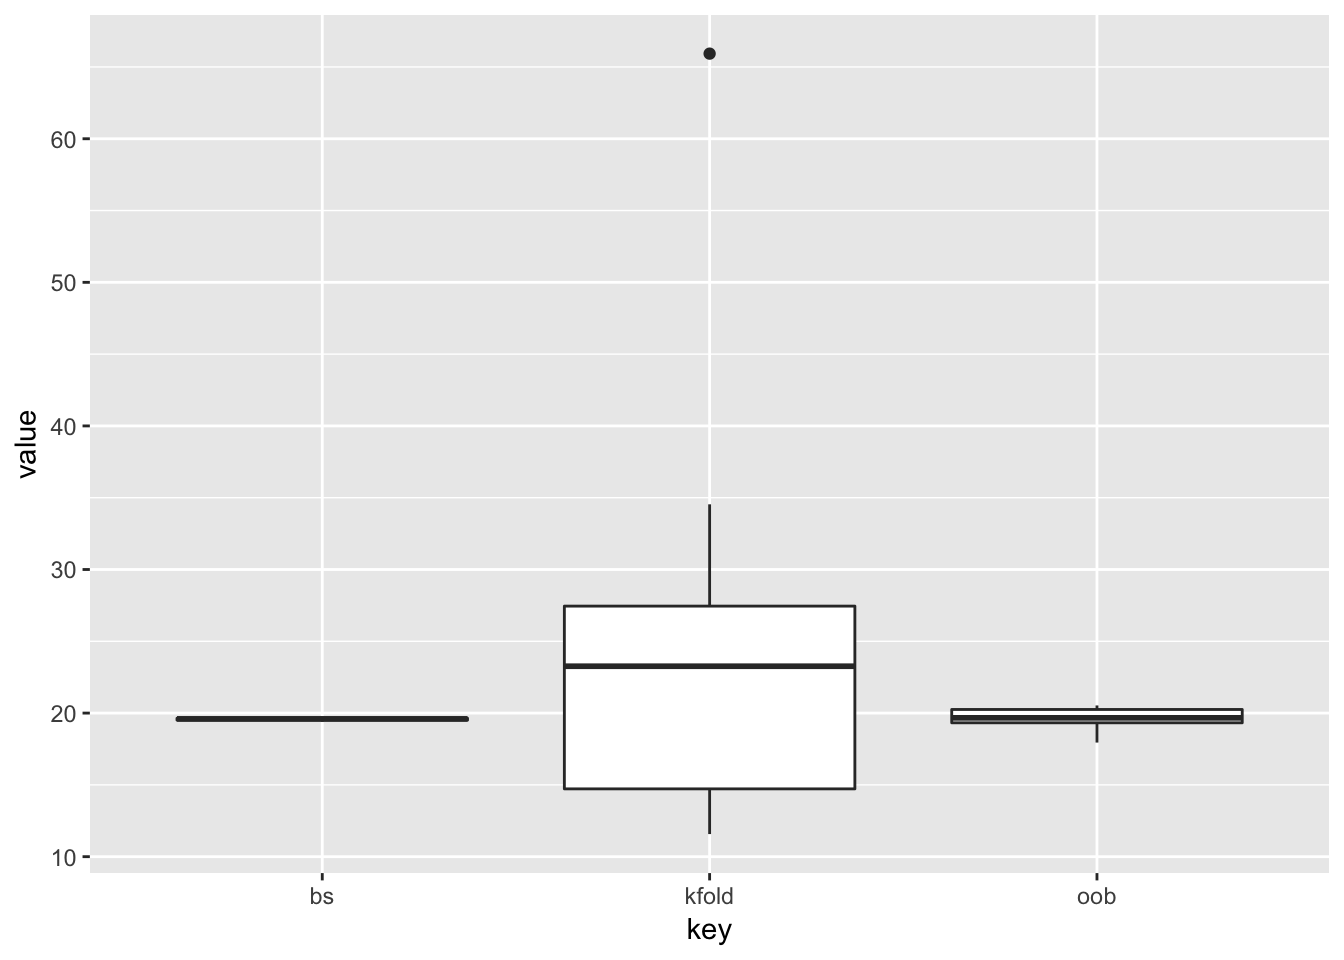
\includegraphics{comp_stats_summary_files/figure-latex/unnamed-chunk-8-1.pdf}

\subsection{Parameter Tuning}\label{parameter-tuning}

We want to use the scheme k-fold cross validation for parameter tuning
with a lasso. We first calculate the test set error for \emph{one} value
of lamda (as we did above). Then, change the value of lamda and
recompute the model and then test set error, so that the test set error
becomes a function of lamda, as depicted below.

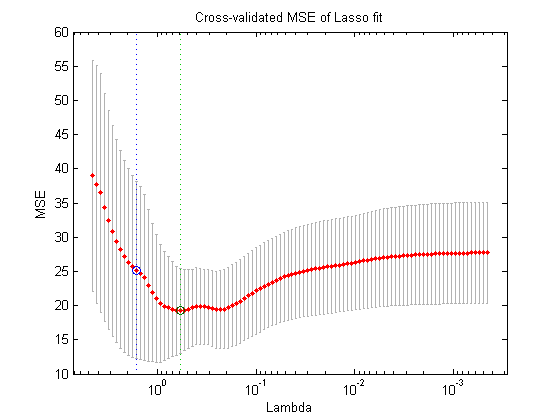
\includegraphics[width=650px]{figures/lasso_cv}

Then pick an optimal lamda, e.g.~the one with the lowest test error (a
bit arbitrary) or one according to some other rule (e.g.~pick the least
complex model that is within one standard error of the best model).

\begin{Shaded}
\begin{Highlighting}[]
\CommentTok{#' Given lambda, compute the test set error with k folds}
\NormalTok{find_lambda_kfold_one <-}\StringTok{ }\NormalTok{function(lambda, k, n, .data, ...) \{}
  \NormalTok{x_test <-}\StringTok{ }\KeywordTok{get_k_fold_test}\NormalTok{(k, n)}
  \NormalTok{x_train  <-}\StringTok{ }\KeywordTok{get_complement}\NormalTok{(x_test, n)}
  \KeywordTok{map2_dbl}\NormalTok{(x_test, x_train, ge_ridge, }\DataTypeTok{lambda =} \NormalTok{lambda, }\DataTypeTok{.data =} \NormalTok{.data, ...) %>%}
\StringTok{    }\KeywordTok{mean}\NormalTok{()}
\NormalTok{\}}

\CommentTok{#' Given a sequence of lambdas, return the corresponding test set errors}
\NormalTok{find_lambda_kfold <-}\StringTok{ }\NormalTok{function(seq, k, .data) \{}
  \NormalTok{cv <-}\StringTok{ }\KeywordTok{map_dbl}\NormalTok{(seq, find_lambda_kfold_one, }
                \DataTypeTok{k =} \NormalTok{k, }\DataTypeTok{n =} \KeywordTok{nrow}\NormalTok{(.data), }\DataTypeTok{.data =} \NormalTok{.data)}
  \NormalTok{results <-}\StringTok{ }\KeywordTok{data_frame}\NormalTok{(}\DataTypeTok{lambda =} \NormalTok{seq, }\DataTypeTok{cv_score =} \NormalTok{cv)}
  \NormalTok{results}
\NormalTok{\}}
\end{Highlighting}
\end{Shaded}

We are almost done. Let us now compute the test set error that we use as
an approximation of the generalization error and plot it against
different values of lamda.

\begin{Shaded}
\begin{Highlighting}[]
\KeywordTok{find_lambda_kfold}\NormalTok{(}\DataTypeTok{seq =} \KeywordTok{seq}\NormalTok{(}\DecValTok{5}\NormalTok{, }\DecValTok{30}\NormalTok{, }\DataTypeTok{by =} \DecValTok{3}\NormalTok{), }\DecValTok{100}\NormalTok{, ozone) %>%}
\StringTok{  }\KeywordTok{ggplot}\NormalTok{(}\KeywordTok{aes}\NormalTok{(}\DataTypeTok{x =} \NormalTok{lambda, }\DataTypeTok{y =} \NormalTok{cv_score)) +}\StringTok{ }
\StringTok{  }\KeywordTok{geom_line}\NormalTok{()}
\end{Highlighting}
\end{Shaded}

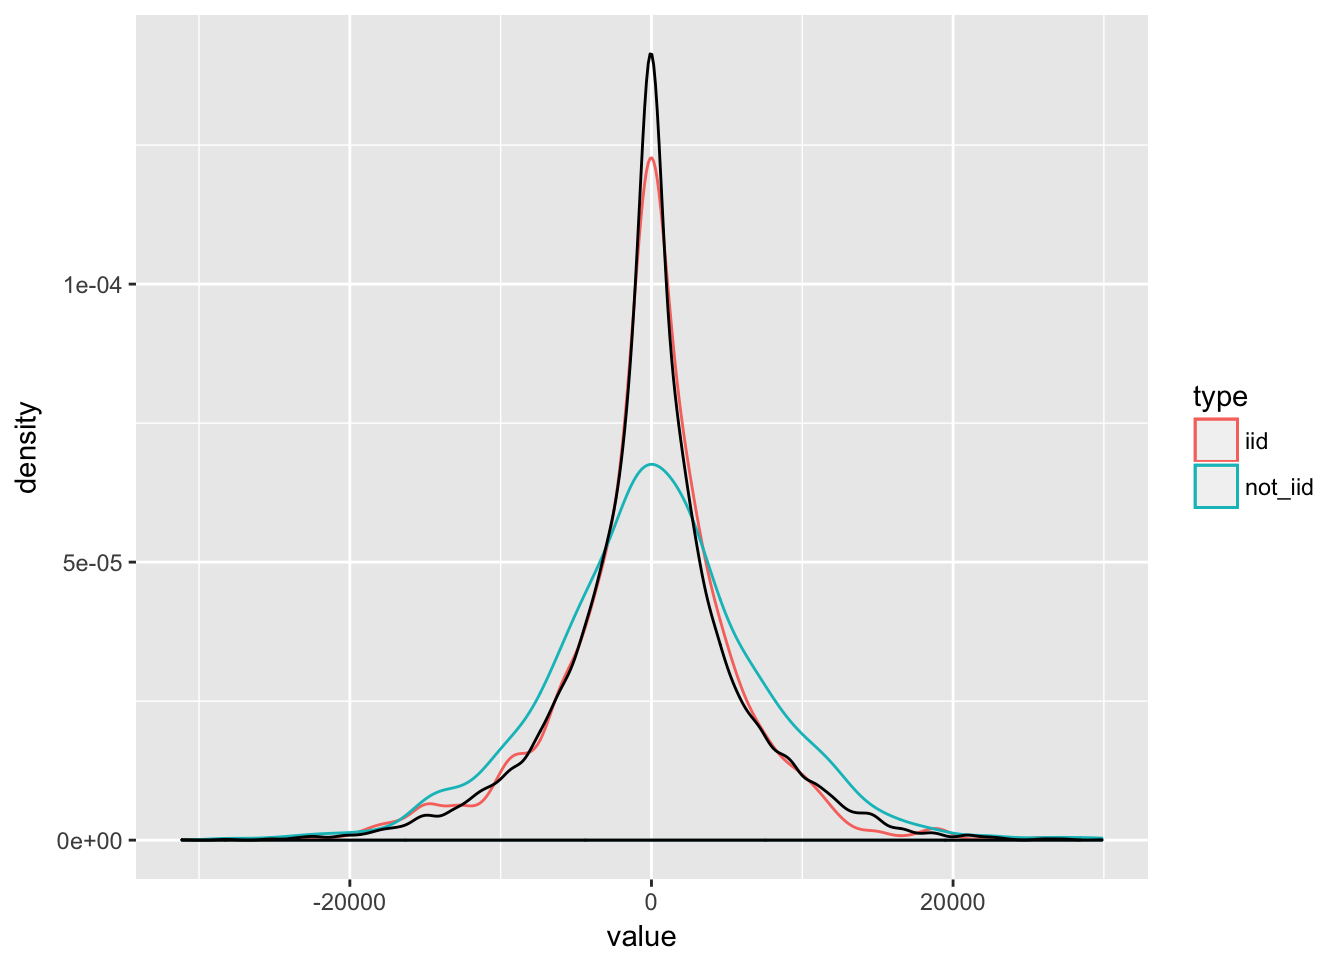
\includegraphics{comp_stats_summary_files/figure-latex/unnamed-chunk-11-1.pdf}

That looks reasonable. We could improve on that by also showing the
distribution of the test set error at various lambadas. This could by
done by altering \texttt{find\_lambda\_kfold\_one()} to not return the
mean, but also the upper and lower 95\% confidence interval.

\chapter{Bootstrap}\label{bootstrap}

\begin{itemize}
\tightlist
\item
  Bootstrap can be summarized as ``simulating from an estimated model''
\item
  It is used for inference (confidence intervals / hypothesis testing)
\item
  It can also be used for estimating the predictive power of a model
  (similarly to cross validation) via out-of-bootstrap generalization
  error
\end{itemize}

\section{Motivation}\label{motivation}

Consider i.i.d. data.
\[ Z_1, .. Z_n \sim\ P \;\; with \; \;Z_i = (X_i, Y_i)\] And assume a
statistical procedure \[ \hat{\theta} = g(Z_1, ..., Z_n) \] \(g(\cdot)\)
can be a point estimator for a regression coefficient, a non-parametric
curve estimator or a generalization error estimator based on one new
observation, e.g.
\[ \hat{\theta}_{n+1} = g(Z_1, ..., Z_{n}, Z_{new}) = (Y_{new} - m_{Z_1, ..., Z_{n}}(X_{new}))^2 \]
To make inference, we want to know the distribution of \(\hat{\theta}\).
For some cases, we can derive the distribution analytically if we know
the distribution \(P\). The central limit theorem states that the sum of
random variables approximates a normal distribution with
\(n \rightarrow \infty\). Therefore, we know that the an estimator for
the mean of the random variables follows the normal distribution.
\[ \hat{\theta}_{n} = n^{-1}\sum x_i \sim N(\mu_x, \sigma_x^2 / n) \; \; \; n \rightarrow \infty \]
for \emph{any} \(P\). However, if \(\hat{\theta}\) does not involve the
sum of random variables, and the CLT does not apply, it's not as
straightforward to obtain the distribution of \(\hat{\theta}\). Also, if
\(P\) is not the normal distribution, but some other distribution, we
can't find the distribution of \(\hat{\theta}\) easily. The script
mentions the median estimator as an example for which the variance
already depends on the density of \(P\). Hence, deriving properties of
estimators analytically, even the asymptotic ones only, is a pain.
Therefore, if we knew \(P\), we could simply simulate many times and get
the distribution of \(\hat{\theta}\) this way. That is, draw many
\(({X_i}^*, {Y_i}^*)\) from that distribution and compute
\(\hat{\theta}\) for each draw.

The problem is that we don't know \(P\). But we have a data sample that
was generated from \(P\). Hence, we can instead take the
\textbf{empirical} distribution \(\hat{P}\) that places probability mass
of \(1/n\) on each observation, draw a sample from this distribution
(which is simply drawing uniformly at random from our sample with
replacement) and compute our estimate of interest from this sample.
\[ \hat{\theta}^{*} = g({Z_1}^{*}, ..., {Z_{new}}^{*})\] We can do that
many times to get an approximate distribution for \(\hat{\theta}\). A
crucial assumption is that \(\hat{P}\) reassembles \(P\). If our data is
not i.i.d, this may not be the case and hence bootstrapping might be
misleading. Below, we can see that i.i.d. sampling (red line)
reassembles the true distribution (black line) quite well, whereas
biased sampling (blue line) obviously does not. We produce a sample that
places higher probability mass on the large (absolute) values.

\begin{Shaded}
\begin{Highlighting}[]
\KeywordTok{library}\NormalTok{(}\StringTok{"tidyverse"}\NormalTok{)}
\NormalTok{pop <-}\StringTok{ }\KeywordTok{data_frame}\NormalTok{(}\DataTypeTok{pop =} \KeywordTok{rnorm}\NormalTok{(}\DecValTok{10000}\NormalTok{) *}\StringTok{ }\DecValTok{1}\NormalTok{:}\DecValTok{10000}\NormalTok{) }
\NormalTok{iid <-}\StringTok{ }\KeywordTok{sample}\NormalTok{(pop$pop, }\DecValTok{1000}\NormalTok{) }\CommentTok{# sample iid}

\CommentTok{# sample non-iid: sample is biased towards high absolute values}
\NormalTok{ind <-}\StringTok{ }\KeywordTok{rbinom}\NormalTok{(}\DecValTok{10000}\NormalTok{, }\DataTypeTok{size =} \DecValTok{1}\NormalTok{, }\DataTypeTok{prob =} \KeywordTok{seq}\NormalTok{(}\DecValTok{0}\NormalTok{, }\DecValTok{1}\NormalTok{, }\DataTypeTok{length.out =} \DecValTok{10000}\NormalTok{)) }
\NormalTok{not_iid <-}\StringTok{ }\NormalTok{pop$pop[}\KeywordTok{as.logical}\NormalTok{(ind)] }\CommentTok{# get sample}
\NormalTok{not_iid <-}\StringTok{ }\KeywordTok{sample}\NormalTok{(not_iid, }\DecValTok{1000}\NormalTok{) }\CommentTok{# reduce sample size to 1000}

\NormalTok{out <-}\StringTok{ }\KeywordTok{data_frame}\NormalTok{(}\DataTypeTok{iid =} \NormalTok{iid, }\DataTypeTok{not_iid =} \NormalTok{not_iid) %>%}
\StringTok{  }\KeywordTok{gather}\NormalTok{(type, value, iid, not_iid)}
\KeywordTok{ggplot}\NormalTok{(out, }\KeywordTok{aes}\NormalTok{(}\DataTypeTok{x =} \NormalTok{value, }\DataTypeTok{color =} \NormalTok{type)) +}\StringTok{ }
\StringTok{  }\KeywordTok{geom_density}\NormalTok{() +}\StringTok{ }
\StringTok{  }\KeywordTok{geom_density}\NormalTok{(}\KeywordTok{aes}\NormalTok{(}\DataTypeTok{x =} \NormalTok{pop, }\DataTypeTok{color =} \OtherTok{NULL}\NormalTok{), }\DataTypeTok{data =} \NormalTok{pop)}
\end{Highlighting}
\end{Shaded}

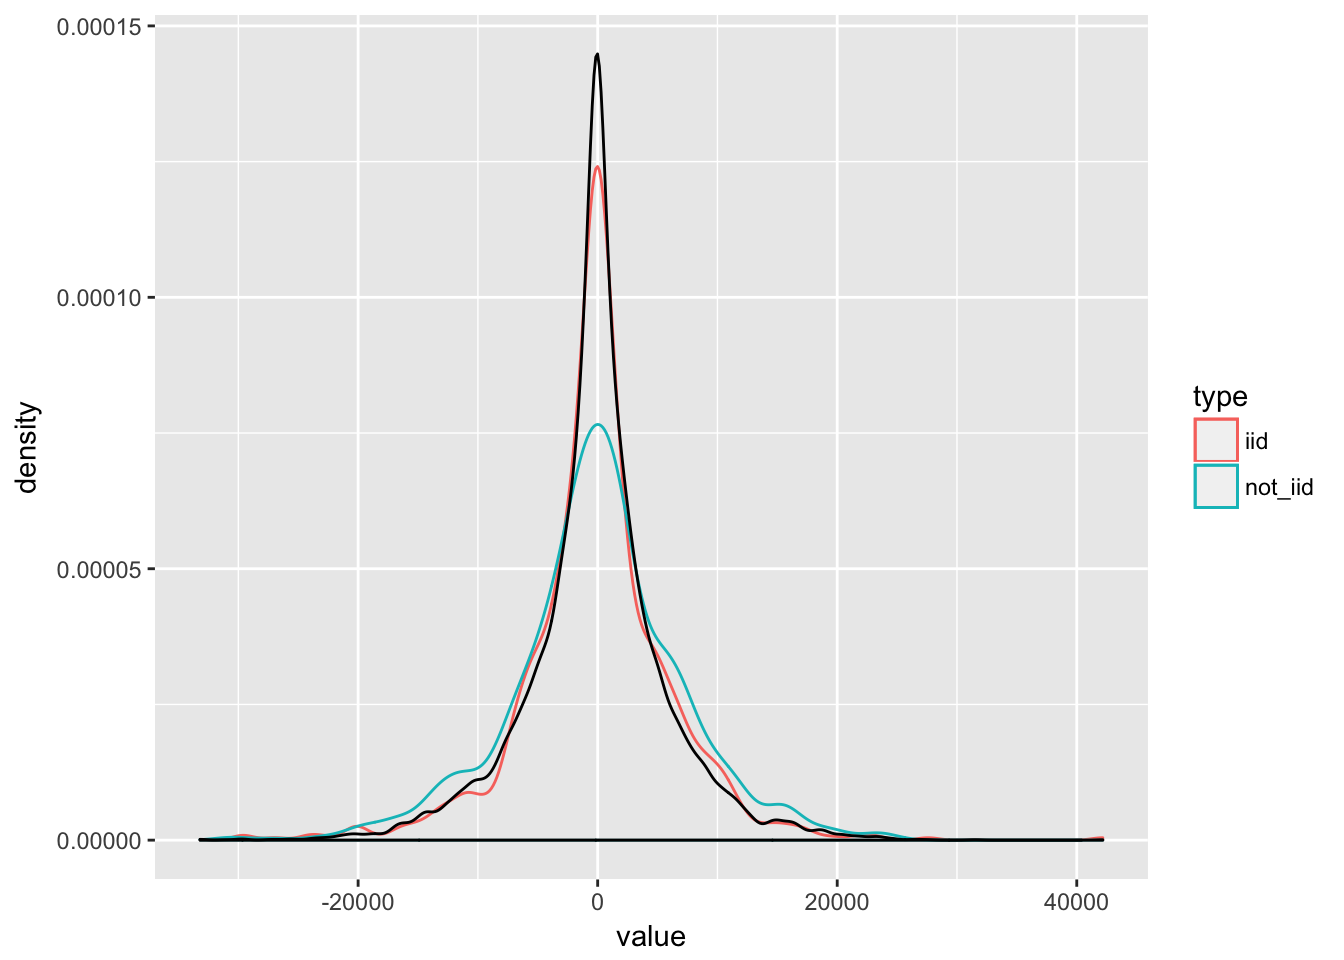
\includegraphics{comp_stats_summary_files/figure-latex/unnamed-chunk-12-1.pdf}

We can summarize the bootstrap procedure as follows.

\begin{itemize}
\tightlist
\item
  draw a bootstrap sample \({Z_1}^{*}, ..., {Z_{n}}^{*}\)
\item
  compute your estimator \({\hat{\theta}}^*\) based on that sample.
\item
  repeat the first two steps \(B\) times to get bootstrap estimators
  \({\hat{\theta}_1}^*, ..., {\hat{\theta}_B}^*\) and therefore an
  estimate of the distribution of \(\hat{\theta}\).
\end{itemize}

Use the \(B\) estimated bootstrap estimators as approximations for the
bootstrap expectation, quantiles and so on.
\(\mathbb{E}[\hat{\theta}^*_n] \approx B^{-1}\sum\limits_{j = 1}^n \hat{\theta}^{* j}_n\)

\section{The Bootstrap Distribution}\label{the-bootstrap-distribution}

With \(P^*\), we denote the bootstrap distribution, which is the
conditional probability distribution introduced by sampling i.i.d. from
the empirical distribution \(\hat{P}\). Hence, \(P^*\) of
\({\hat{\theta}}^*\) is the distribution that arises from sampling
i.i.d. from \(\hat{P}\) and applying the transformation \(g(\cdot)\) to
the data. Conditioning on the data allows us to treat \(\hat{P}\) as
fixed.

\section{Bootstrap Consistency}\label{bootstrap-consistency}

The bootstrap is is called consistent if
\[ \mathbb{P}[a_n(\hat{\theta} - \theta) \leq x ] - \mathbb{P}[a_n(\hat{\theta}^* - \hat{\theta}) \leq x ] \rightarrow 0 \;\; (n \rightarrow \infty)\]
Consistency of the bootstrap typically holds if the limiting
distribution is normal and the samples \(Z_1, .., Z_n\) are i.i.d.
Consistency of the bootstrap implies consistent variance and bias
estimation:

\[ \frac{Var^* (\hat{\theta}^*)}{Var(\hat{\theta})} \rightarrow 1\]
\[ \frac{\mathbb{E}^* (\hat{\theta}^*) - \hat{\theta}}{\mathbb{E}(\hat{\theta}) - \theta} \rightarrow 1\]
You can think of \(\theta\) as the real parameter and \(\hat{\theta}\)
as the estimate based on a sample. Similarly, in the bootstrap world,
\(\hat{\theta}\) is the \emph{real} parameter, and \(\hat{\theta}^*_i\)
as an estimator of the \emph{real} parameter \(\hat{\theta}\). The
bootstrap world is an analogue of the real world. So in our bootstrap
simulation, we know the \emph{true} parameter \(\hat{\theta}\). From our
simulation, we get many \(\hat{\theta}^*_i\) and can find the bootstrap
expectation
\(\mathbb{E}[\hat{\theta}^*_n] \approx B^{-1}\sum\limits_{j = 1}^n \hat{\theta}^{* j}_n\).
The idea is now to generalize from the \emph{boostrap} world to the
\emph{real} world, i.e.~by saying that the relationship between
\(\hat{\theta}^*\) and \(\hat{\theta}\) is similar to the one between
\(\hat{\theta}\) and \(\theta\).

A simple trick to remember all of this is:

\begin{itemize}
\tightlist
\item
  if there is no hat, add one
\item
  if there is a hat, add a star.
\end{itemize}

\section{Boostrap Confidence
Intervals}\label{boostrap-confidence-intervals}

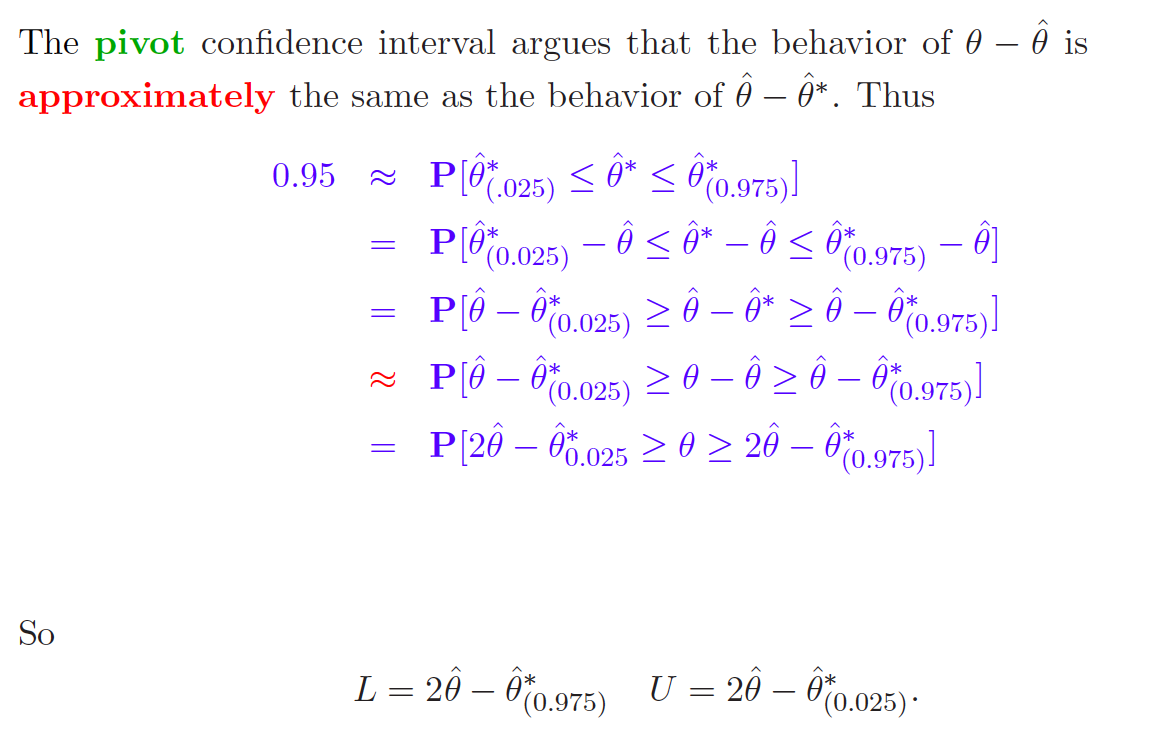
\includegraphics[width=16.08in]{figures/pivot_ci}

Note that there confidence intervals are not simply taking the quantiles
of the bootstrap distribution. The trick is really to make use of the
analogy between the \emph{real} world and the \emph{boostrap} world. So
when we see our bootstrap expectation \(\mathbb{E}[\hat{\theta}^*_n]\)
is way higher than \(\hat{\theta}\), then we also should believe that
our \(\hat{\theta}\) is higher than \(\theta\). The above procedure
accounts for that.

\section{Boostrap Estimator of the Generalization
Error}\label{boostrap-estimator-of-the-generalization-error}

We can also use the bootstrap to estimate the generalization error.
\[ \mathbb{E}[\rho(Y_{new}, m^*(X_{new}))] \]

\begin{itemize}
\tightlist
\item
  We draw a sample \(({Z_1}^*, ..., {Z_n}^*, Z_{new})\) from \(\hat{P}\)
\item
  We compute the bootstrapped estimator \({m(\cdot)}^*\) based on the
  sample
\item
  We estimate \(\mathbb{E}[\rho(Y_{new}, {m^*(X_{new})}^*)]\), which is
  with respect to both training and test data.
\end{itemize}

We can rewrite the generalization error as follows:
\[ \mathbb{E}[\rho(Y_{new}, m^*({X_{new}}^*))] = \mathbb{E}_{train}[E_{test}[\rho({Y_{new}}^*, m^*({X_{new}}^*))| train]]\]
Conditioning on the training data in the inner expectation, \(m(\cdot)\)
is non-random / fixed. The only random component is \({Y_{new}}^*\).
Since we draw from the empirical distribution and place a probability
mass of \(1/n\) on every data point. we can calculate the inner
(discrete) expectation easily via
\(\mathbb{E}(X) = \sum\limits_{j = 1}^n p_j * x_j = n^{-1} \sum\limits_{j = 1}^n x_j\).
The expectation becomes
\[ \mathbb{E}_{train}[n^{-1}\sum\rho(Y_{i}, m^*(X_{i}))] =  n^{-1}\sum\mathbb{E}[\rho(Y_{i}, m^*(X_{i}))]\]

We can see that there is no need to draw \(Z_{new}\) from the data. The
final algorithm looks as follows:

\begin{itemize}
\tightlist
\item
  Draw \(({Z_1}^*, ..., {Z_n}^*)\)
\item
  compute bootstrap estimator \({\hat{\theta}}^*\)
\item
  Evaluate this estimator on all data points and average over them, i.e
  \(err^* = n^{-1} \sum \rho(Y_i, m^*(X_i))\)
\item
  Repeat steps above B times and average all error estimates to get the
  bootstrap GE estimate, i.e. \(GE^* = B^{-1} \sum {err_i}^*\)
\end{itemize}

\section{Out-of-Boostrap sample for estimating the
GE}\label{out-of-boostrap-sample-for-estimating-the-ge}

One can criticize the GE estimate above because some samples are used in
the \textbf{test as well as in the training set}. This leads to
\textbf{over-optimistic estimations} and can be avoided by using the
out-of-bootstrap approach. With this technique, we first generate a
bootstrap sample to compute our estimator and then use the remaining
observations not used in the bootstrap sample to evaluate the estimator.
We do that \(B\) times and the size of the test set may vary. You can
see this as some kind of cross-validation with about 30\% of the data
used as the test set. The difference is that some observations were used
multiple times in the training data, yielding a \textbf{training set
always of size n} (instead of - for example \(n*0.9\) for 10-fold-CV).

\section{Double Boostrap Confidence
Intervals}\label{double-boostrap-confidence-intervals}

Confidence intervals are almost never exact, meaning that
\[\mathbb{P}[\theta \in I^{**}(1-\alpha)] = 1-\alpha + \Delta\] Where
\(I^{**}(1-\alpha)\) is a \(\alpha\)-confidence interval. However, by
changing the \emph{nominal} coverage of the confidence interval, it is
possible to make the actual coverage equal to an arbitrary value, i.e

\[ \mathbb{P}[\theta \in I^{**}(1-\alpha')] = 1-\alpha\] The problem is
that \(\alpha'\) is unknown. But another level of bootstrap can be used
to \textbf{estimate} \(\alpha\), denoted by \(\hat{\alpha}\), which
typically achieves
\[\mathbb{P}[\theta \in I^{**}(1-\hat{\alpha}')] = 1- \alpha + \Delta'\]
with \(\Delta' < \Delta\)

To implement a double bootstrap confidence interval, proceed as follows:

\begin{enumerate}
\def\labelenumi{\arabic{enumi}.}
\tightlist
\item
  Draw a bootstrap sample \(({Z_1}^*, ..., {Z_n}^*)\).

  \begin{enumerate}
  \def\labelenumii{\alph{enumii}.}
  \tightlist
  \item
    From this sample, draw B second-level bootstrap samples and compute
    the estimator of interest and \emph{one} confidence interval
    \(I^{**}(1-\alpha)\) based on B second-level bootstrap samples.
  \item
    evaluate whether \(\hat{\theta}\) lays within the bootstrap
    confidence interval from a.
    \(cover^*(1-\alpha) = 1_{[\hat{\theta} \in I^{**}(1-\alpha)]}\)
  \end{enumerate}
\item
  Repeat the above M times to get \(cover^{* 1}, ..., cover^{* M}\) and
  hence approximate \(\mathbb{P}[\theta \in I^{**}(1-\alpha)]\) with
  \[ p^*(\alpha) = M^{-1} \sum\limits_{m = 1}^M cover^{* m}\]
\item
  Vary \(\alpha\) in all of the steps above to find \(\alpha'\) so that
  \(p^*(\alpha') = 1- \alpha\)
\end{enumerate}

Question here (see Google docs)

\section{Three Versions of Boostrap}\label{three-versions-of-boostrap}

\begin{itemize}
\tightlist
\item
  So far, we discussed the \textbf{fully non-parametric} bootstrap,
  which is simulating from the empirical distribution.
\item
  On the other extreme of the scale, there is the \textbf{parametric
  bootstrap}.
\item
  The middle way is the model-based bootstrap
\end{itemize}

\subsection{Non-parametric
Regression}\label{non-parametric-regression-1}

We draw a bootstrap sample \(({Z_1}^*, ..., {Z_n}^*) \sim \hat{P}\),
i.e.~we sample from the \emph{empirical distribution} data with
replacement.

\subsection{Parametric Boostrap}\label{parametric-boostrap}

Here, we assume the data are realizations from a \emph{known}
distribution \(P\), which is is determined up to some unknown parameter
(vector) \(\theta\). That means we sample
\((Z_1, ..., Z_n) \sim P_{\hat{\theta}}\). For example, take the
following regression model \(y = X\beta + \epsilon\) where we know the
errors are Gaussian.

\begin{enumerate}
\def\labelenumi{\arabic{enumi}.}
\tightlist
\item
  We can estimate our regression model, obtain residuals and compute the
  mean (which is zero) and the standard deviation of them.
\item
  To generate a bootstrap sample, we simulate residuals \(\epsilon^*\)
  from \(N(0, \hat{\mu})\) and
\item
  Add them to our observed data, i.e.~we obtain
  \(({Y_1}^*, ..., {Y_n}^*)\) from \(X\beta + \epsilon^*\). Hence, the
  final bootstrap sample we use is
  \((x_1, {Y_1}^*), ..., (x_1, {Y_n}^*))\) where the \(x_i\) are just
  the observed data.
\item
  We can compute bootstrap estimates \(\hat{\beta}^*\), the bootstrap
  expectation \(\mathbb{E}^*[\beta*]\) as well as confidence intervals
  for the regression coefficients or generalization errors just as shown
  in detail above. The difference is only \emph{how} the bootstrap
  sample is obtained.
\end{enumerate}

Similarly, for time series data, we may assume an AR(p) model.

\begin{enumerate}
\def\labelenumi{\arabic{enumi}.}
\tightlist
\item
  Initializing \({X_0}^*, ..., {X_{-p+1}}^*\) with \(0\).
\item
  Generate random noise \({\epsilon_1}^*, ..., {\epsilon_{n+m}}^*\)
  according to \(P_{\hat{\theta}}\).
\item
  Construct our time series
  \({X_t}^* = \sum\limits_{j = 1}^p \hat{\theta}{X_{t-j}}^* + {\epsilon_t}^*\)
  \((X_1, ..., X_{n+m})\)
\item
  Throw away the first \(M\) observations that were used as fade-in.
\item
  Proceed with the B bootstrap samples \(({X_1}^*, ..., {X_n}^*)\) as
  outlined above for the non-parametric bootstrap to obtain coefficient
  estimates for \(\theta\), confidence intervals or estimating the
  generalization error of the model.
\end{enumerate}

\subsection{Model-Based Bootstrap}\label{model-based-bootstrap}

The middle way is the model based bootstrap. As with the parametric
bootstrap, we assume to know the model, e.g. \(y = m(x) + \epsilon\)
(where \(m(\cdot)\) might be a non-parametric curve estimator), but we
do not make an assumption about the error distribution. Instead of
generating \(\epsilon^*\) from the known distribution with unknown
parameters (\(\epsilon^* \sim P_{\hat{\theta}}\), as in the parametric
bootstrap)), we draw them with replacement from the \emph{empirical}
distribution. To sum it up, these are the steps necessary:

\begin{enumerate}
\def\labelenumi{\arabic{enumi}.}
\tightlist
\item
  Estimate \(\hat{m(\cdot)}\) from all data.
\item
  Simulate \({\epsilon_1}^*, ..., {\epsilon_n}^*\) by drawing from
  \(\hat{P}\) with replacement.
\item
  Obtain \(({Y_1}^*, ..., {Y_n}^*)\) from \(\hat{m}(x) + \epsilon^*\).
  As for the parametric bootstrap, the final bootstrap sample we use is
  \((x_1, {Y_1}^*), ..., (x_n, {Y_n}^*))\) where the \(x_i\) are just
  the observed data.
\item
  Again, you can use the bootstrap samples as for the other two methods.
\end{enumerate}

\section{Conclusion}\label{conclusion}

Which version of the bootstrap should I use? The answer is classical. If
the parametric model fits the data very well, there is no need to
estimate the distribution explicitly. Also, if there is very little
data, it might be very difficult to estimate \(P\). On the other hand,
the non-parametric bootstrap is less sensitive to model-misspecification
and can deal with arbitrary distributions (? is that true?).

\chapter{Classification}\label{classification}

\section{Indirect Classification - The Bayes
Classifier}\label{indirect-classification---the-bayes-classifier}

In classification, the goal is to assign observations to a group.
Similar to regression, where we have \(m(x) = E[Y | X = x]\), we want to
assign class probabilities to the observations
\[\pi_j (x) = P[Y = j | X = x] \;\;\;  (j = 0,1, ..., J-1)  \]
\emph{Def}: A classifier maps A multidimensional input vector to a class
label. Or mathematically:
\(C: \mathbb{R}^p \rightarrow \{0, ..., J-1\}\) The quality of a
classifier is measured via the zero-one test-error.
\[\mathbb{P}[C(X_{new}) \neq Y_{new}] \]

The optimal classifier with respect to the zero-one Error is the Bayes
Classifier. It classifies an observation to the group for which the
predicted probability was the highest.
\[ C_{bayes}(x) = \arg\max_{0<j<J-1}\pi_j(x)\] Hence, the Bayes
Classifier is a point-wise classifier. For the Bayes Classifier, the
zero-one test error is known as the \emph{Bayes Risk}.
\[ \mathbb{P}[C_{Bayes}(X_{new}) \neq Y_{new}]\]

In practice, \(\pi_j(\cdot)\) is unknown (just as the MSE in regression
is unknown) and hence, the the Bayes Classifier and Risk is unknown too.
However, we can estimate \(\pi_j(\cdot)\) from the data and plug it in
the Bayes Classifier. \[\hat{C}(X) = \arg\max_{0<j<J-1}\hat{\pi}_j(x)\]
This is an indirect estimator, since we first estimate the class
probabilities \(\pi_j(\cdot)\) for each observation \(x\) and then
assign the class to it for which the probability was the highest.
Question how is that more indirect than Discriminant analysis? Don't we
use the Bayes classifier in the end?

\section{Direct Classification - The Discriminant
View}\label{direct-classification---the-discriminant-view}

\subsection{LDA}\label{lda}

One example for a direct classification is discriminant analysis. Using
Bayes Theorem
\[ \mathbb{P}[Y = j | X] = \frac{\mathbb{P}[X = x | y = j]}{\mathbb{P}[X = x]}*\mathbb{P}[Y = j] \]
And assuming

\[ (X| Y) \sim N_p(\mu_j, \Sigma); \;\; \sum\limits_{k = 0}^{J-1}p_k = 1\]

We can write
\[ \mathbb{P}[Y = j | X = x] = \frac{f_{ x | Y = j } * p_j}{\sum\limits_{k = 0}^{J-1} f_{x | Y = k} * p_k} \]
Note that there is no distributional assumption on \(Y\) so far. You can
estimate
\[\mu_j = \sum\limits_{i = 1}^n{x_i*1_{Y_i = j}} / 1_{Y_i = j}\] and
\[\Sigma = \frac{1}{n-j}\sum\limits_{j = 0}^{J-1}\sum\limits_{i = 1}^n(x_i - \mu_j)(x_i - \mu_j)'\;1_{Y_i = j} \]
Note that the means of the response of the groups are different, but the
covariance structure is the same for all of them. We now also need to
estimate \(p_j\). A straight-forward way is
\[ \hat{p}_j = n^{-1}\sum\limits_{i = 1}^n{1_{[Y_i = j]}} = \frac{n_j}{n} \]

From here, you can easily compute the classifier (as done in the
exercise) by maximizing the log-likelihood. Then, you can derive the
decision boundary by using \(\delta_j - \delta_k = 0\). In a two
dimensional predictor space with two classes, the decision boundary is a
line. Every combination of the two predictors on one side of the line
will result in a prediction of class one, everything on the other side
of the line of class two. Note that both the decision function (and
hence the decision boundary) are linear in x.

\subsection{QDA}\label{qda}

Quadratic discriminant analysis loosens the assumption of shared
covariance matrices, namely each group has their own covariance matrix.
This leads to quadratic decisions functions \(\delta\) and hence to
non-linear decision boundaries. QDA is more flexible but for high \(p\),
the problem of over-fitting can occur, since the number of variables to
estimate is \(J*p(p+1)\) variable for the covariance matrix only
(instead of \(p*(p+1)\) for LDA.

\section{Indirect Classification - The View of Logistic
Regression}\label{indirect-classification---the-view-of-logistic-regression}

There are also ways to come up with indirect assignment of the class
label, namely via the Bayes classifier
\(\hat{C}(X) = \arg\max_{0<j<J-1}\hat{\pi}_j(x)\). The logistic model
for \(\pi_j(x) = \mathbb{P}(Y = j | X = x)\) is
\(\log(\frac{\pi_j(x)}{1-\pi_j(x)}) = g(\cdot)\) or
\(\pi_j(x) = \frac{e^{g(\cdot)}}{1+ e^{g(\cdot)}}\) equivalently. That
model maps the real value \(g(\cdot)\) can take to the interval
\((0, 1)\), which gives a natural interpretation of the response as a
probability. Note that we want the transformation to be monotone so the
mapping is invertible. The response variable \(Y_1, ..., Y_n\) are
distributed according to a Bernoulli distribution, i.e..
\(Y_1, ..., Y_n \sim \textrm{Bernulli}(\pi(x_i))\). The logistic model
belongs to the class of generalized linear models. These models have
three characteristics:

\begin{itemize}
\tightlist
\item
  A link function (in our case the logit function
  \(\log(\frac{\pi_j(x)}{1-\pi_j(x)}) = g(x)\)).
\item
  A response distribution (i.e.~Bernoulli)
\item
  The concrete form of \(g(\cdot)\) (in logistic regression most often
  just a linear model \(g(x) = \sum\limits_{j = 1}^p \beta_j x_j\)).
\end{itemize}

This allows us to write down the likelihood of the logistic model

\begin{equation} 
\begin{split}
L(\beta, (x_1, Y_1), ..., (x_n, Y_n))&  = \prod\limits_{i = 1}^n \mathbb{P}(Y_i = y_i)\\
 & =\prod\limits_{i = 1}^n \pi(x_i)^{Y_i-1}(1-\pi(x_i))^{Y_i-1}\\
\log(L(\cdot) & = \sum\limits_{i = 1}^n Y_i \pi(x_i) + (1 - Y_i) (1 - \pi(x_i))
\end{split}
\label{eq:var-beta}
\end{equation}

There is no closed-form solution for the above problem, hence we need to
rely on gradient descent to find the maximum likelihood solution. You
can fit a logistic regression model in R as follows:

\begin{Shaded}
\begin{Highlighting}[]
\CommentTok{# fit the model}
\NormalTok{fit <-}\StringTok{ }\KeywordTok{glm}\NormalTok{(response~predictors, }\DataTypeTok{data =} \NormalTok{my_data, }\DataTypeTok{family =} \StringTok{"binomial"}\NormalTok{)}
\CommentTok{# predict}
\NormalTok{prediction <-}\StringTok{ }\KeywordTok{predict}\NormalTok{(fit, }\DataTypeTok{newdata =} \NormalTok{my_data, }\DataTypeTok{type =} \StringTok{"response"}\NormalTok{) >}\StringTok{ }\FloatTok{0.5}
\CommentTok{# evaluate in-sample}
\KeywordTok{mean}\NormalTok{(prediction ==}\StringTok{ }\NormalTok{my_data$response)}
\end{Highlighting}
\end{Shaded}

\section{Discriminant Analysis or Logistic
Regression?}\label{discriminant-analysis-or-logistic-regression}

\begin{itemize}
\tightlist
\item
  The logistic regression assumes the log-odds to be \emph{linear} in
  the predictors, i.e.
  \(\log\Big(\frac{\pi}{1-\pi}\Big) = \sum\limits_{i = 1}^p \beta_i x_i\).
\item
  The discriminant analysis assumes \(X|Y \sim N(\mu_j, \Sigma\), which
  leads to linear model in the decision variables. Hence, the methods
  are \textbf{quite similar}.
\item
  It is quite natural to use factors with logistic regression, while for
  discriminant analysis, it is not very natural (?even not reasonable?).
\item
  Empirically, the two methods yield similar results even under a
  violation of the normality assumption.
\end{itemize}

\textbf{TODO} multinomial likelihood (see footnote.)

\section{Multiclass case (J \textgreater{}
2)}\label{multiclass-case-j-2}

With logistic regression, you can not model multiclass cases directly,
but indirectly using one of the following methods:

\begin{itemize}
\tightlist
\item
  Encode a J-case problem as J binary problems (one class against the
  rest), that is
\end{itemize}

\begin{equation}
  Y_i^{(j)} = \begin{cases}
        1 \;\;\ \text{if} \;\;\ Y_i = j
        \\
        0 \;\;\ \text{else}.
        \end{cases}
 \end{equation}

For each case you want to label, you will obtain \(J-1\) probability
estimates, i.e.
\(\pi_j(x) = \frac{\exp\big(\sum\beta^{(j)}_jx_j\big)}{1 + \exp\big(\sum\beta^{(j)}_jx_j\big)}\).
They don't sum up to one necessarily, but you can normalize to obtain
normed probabilities. Then, use the Bayes classifier to choose the class
label (\(\arg\max_{0 < j < J-1} \pi_j\))

\begin{itemize}
\tightlist
\item
  Similarly, you can also model \emph{all against the reference},
  \(\log(\frac{\pi_1}{\pi_0})\). This might be helpful when we want to
  compare different group memberships with a reference group. For
  example in clinical trials, we want to compare how many times more
  likely someone belongs to group \emph{ill with disease A} than
  \emph{healthy} (the reference).
\item
  You can also look at pair-wise comparisons. Choose two groups you want
  to compare, drop all observations that don't belong to one of the two
  groups and estimate the model. There are \(\binom{J}{2}\) possible
  models with all models potentially having different number of
  observations.
\item
  In the special case of \textbf{ordered groups}, the correct model is
  often proportional odds model that models
  \[\text{logit}(\mathbb{P}(Y < k |X) = \alpha_k + g(\cdot))\] with
  \(\alpha_1 < \alpha_2 < \text{...} < \alpha_{J-1}\). The log odds are
  proportional, which becomes obvious if we take \(e\) to the power of
  the above equation. Check
  \href{http://data.library.virginia.edu/fitting-and-interpreting-a-proportional-odds-model/}{this}
  webpage for more information. Note that proportionality in the log
  odds does \emph{not} mean proportionality in the probabilities, since
  they are only linked through a non-linear mapping (the logistic
  transformation).
\end{itemize}

\chapter{Flexible regression and classification
methods}\label{flexible-regression-and-classification-methods}

The curse of dimensionality makes it very hard to estimate fully
non-parametric regression function \(\hat{m} = \mathbb{E}[Y|X = x]\) or
classification function \(\hat{\pi}_j = \mathbb{P}[Y = j | X = x]\).
Hence, by making some (reasonable) structural assumptions, we can
improve our models significantly. Generally, we consider the mapping
\(\mathbb{R}^p \rightarrow \mathbb{P}\) via the function \(g(\cdot)\)
for both the regression and the classification problem.

\section{Additive Models}\label{additive-models}

\subsection{Structure}\label{structure}

One assumption we can make is to assume a particular functional form of
\(g(\cdot)\), namely an \emph{additive}. That is
\[g_{add}(x) = \mu + \sum\limits_{j = 1}^pg(x_j) \] \(E[g(x_j)] = 0\) is
required to make the model identifiable only. Note that we have not
placed any assumption on \(g(x_j)\) yet, that is, \(g(x_j)\) can be
fully non-parametric, but each dimension is mapped separately. In other
words every \(g(x_j) \;\; j = 1, ..., p\) models one input dimension and
mapping of input to output is obtained by summing the transformed inputs
up. This eliminates the possibility of \textbf{interaction effects}.

\subsection{Fitting Procedure}\label{fitting-procedure}

Additive models can be estimated with a technique called back-fitting.
However, the model can be estimated with any non-parametric method for
one-dimensional smoothing. Here is the receipt:

\begin{itemize}
\tightlist
\item
  since we assume an additive model, we need to initialize all \(p\)
  components of it with zero, that is setting
  \(g_j(\cdot) = 0 \;\; j = 1,..., p\) plus setting
  \(\mu = n^{-1}\sum Y_i\). * Then we fit one-dimensional smoother
  repeatedly, that is solving the one-dimensional smoothing problem
  \(Y - \mu - \sum\limits_{j \neq k}\hat{g}_j = \hat{g}_j(x_j)\), or put
  differently \(\hat{g}_j = S_j(Y - \mu1 - \sum\limits_{j \neq k}g_j)\).
  This has to be done repeatedly for \(j = 1, ..., p, 1, ..., p\) etc.
\item
  Stop iterating when functions don't change much anymore, that is, when
  the following quantity is less than a certain tolerance.
  \[\frac{|\hat{g}_{i, new} - \hat{g}_{i, old}|}{|\hat{g}_{i, old}|}\]
\item
  Normalize the functions by subtracting the mean from them:
  \[\tilde{g}_j = \hat{g}_j - n^{-1} \sum\limits_{i = 1}^n \hat{g}_j(x_{ij})\]
\end{itemize}

Back-fitting is a \textbf{coordinate-wise} optimization method that
optimizes one coordinate at the time (one \(g(\cdot)\), but can be more
than one parameter), which may be slower in convergence than a general
gradient descent that optimizes all directions simultaneously but also
more robust.

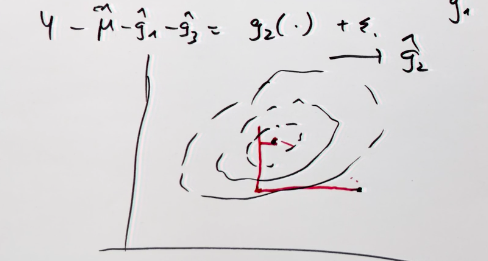
\includegraphics[width=6.78in]{figures/coordinate_wise}

\subsection{Additive Models in R}\label{additive-models-in-r}

You can use the package \textbf{mgcv}

\begin{Shaded}
\begin{Highlighting}[]
\KeywordTok{data}\NormalTok{(}\StringTok{"ozone"}\NormalTok{, }\DataTypeTok{package =} \StringTok{"gss"}\NormalTok{) }
\NormalTok{fit <-}\StringTok{ }\NormalTok{mgcv::}\KeywordTok{gam}\NormalTok{(upo3 ~}\StringTok{ }\KeywordTok{s}\NormalTok{(vdht) +}\StringTok{ }\KeywordTok{s}\NormalTok{(wdsp) +}\StringTok{ }\KeywordTok{s}\NormalTok{(hmdt) +}\StringTok{ }\KeywordTok{s}\NormalTok{(sbtp), }
           \DataTypeTok{data =} \NormalTok{ozone) }

\KeywordTok{plot}\NormalTok{(fit, }\DataTypeTok{pages =} \DecValTok{1}\NormalTok{) }
\end{Highlighting}
\end{Shaded}

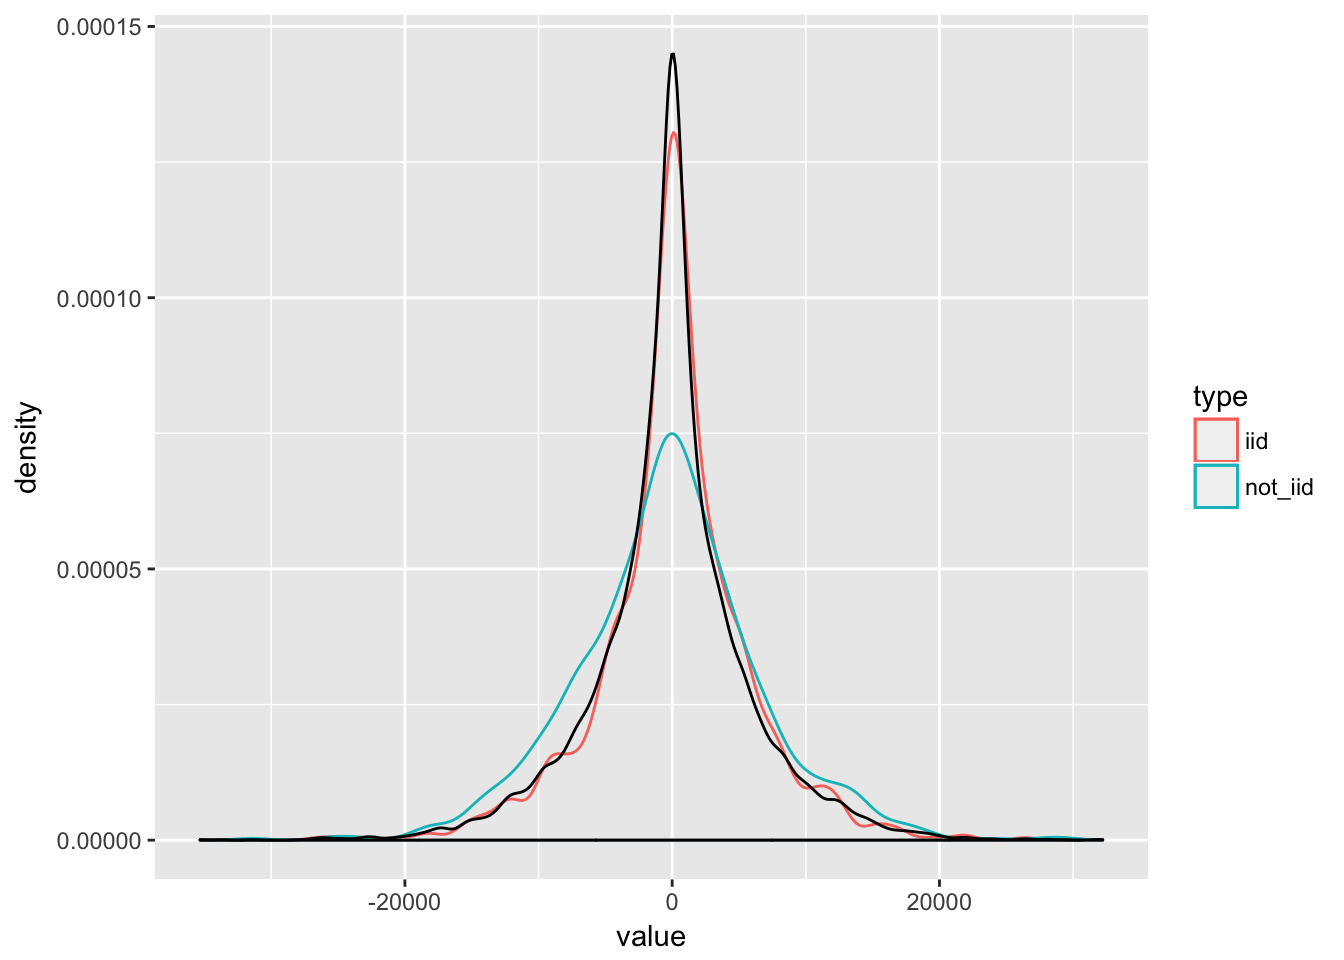
\includegraphics{comp_stats_summary_files/figure-latex/unnamed-chunk-18-1.pdf}

You can see that vdht enters the model almost linearly. That is, with an
increase of one unit of vdht, the predicted 03 value increases linearly.
sbtp is different. Depending on the value of sbtp, the increase in the
predicted value is different. Low sbtp values hardly have an impact on
the response, higher values do.

\section{MARS}\label{mars}

MARS stands for multivariate adaptive regression splines and allows
pice-wise linear curve fitting. In contrast to GAMs, they allow for
interactions between the variables. MARS is very similar to regression
trees, but it has a continuous response. It uses reflected pairs of
basis functions

\begin{equation} 
  (x_j -d)_{+} = \begin{cases} x_j - d \;\;\ \text{if} \;\;\ x_j - d > 0 \\ 
  0 \;\;\ \text{else}. 
  \end{cases} 
\end{equation}

and it counterpart \((d - x_j)_{+}\). The index \(j\) refers to the j-th
predictor variable, d is a knot at one of the \(x_js\). The pool of
basis functions to consider is called \(\mathcal{B}\) and contains all
variables with all potential knots, that is \[
\mathcal{B} = \{(x_j - d)_+ \;\;\; (d - x_j)_+ \;\;\;j = \{1, ..., p\} \;\; d =
\{x_{1j}, ..., x_{nj}\}\}\] The model then is
\[ g(x)  = \mu + \sum\limits_{m =
1}^M\beta_m h_m(x) = \sum\limits_{m = 0}^M\beta_m h_m(x)\] The model
uses forward selection and backward deletion and optimizes some
(generalized) cross-validation criterion. Here is the receipt:

\begin{enumerate}
\def\labelenumi{\arabic{enumi}.}
\tightlist
\item
  initialize \(\mathcal{M} = \{h_0(\cdot) = 1\}\) and estimate
  \(\beta_0\) as the data average of the response
  \(n^{-1}\sum\limits_{i = 1}^n Y_i\).
\item
  for \(r = 1, 2, ...\) search for a new pair of function
  \((h_{2 r-1} \;\;  h_{2 r})\) which are of the form
  \[h_{2 r-1} = (x_j -d)_+ \times h_l\] \[h_{2 r} = (d -
     x_j)_+ \times h_l\] that reduce the residual sum of squares the
  most with some \(h_l\) from \(\mathcal{M}\) that some basis functions
  from \(\mathcal{B}\) does \emph{not} contain \(x_j\). The model
  becomes \[\hat{g}(x) = \sum\limits_{m = 0}^{2r}\hat{\beta}_m
     h_m(x)\] which can be estimated by least squares. Update the set
  \(\mathcal{M}\) to be
  \(\mathcal{M} = \mathcal{M}_{old} \cup \{h_{2r-1}, h_{2r}\}\)
\item
  Iterate the above step until the set \(\mathcal{M}\) becomes
  \emph{large enough}.
\item
  Do backward deletion (\emph{pruning}) by removing the \emph{one}
  function from a reflected pair that increases the residual sum of
  squares the least.
\item
  Stop the pruning when some GCV score reaches its minimum.
\end{enumerate}

From the receipt above, we can see that \(d\)-way interactions are only
possible if a \(d-1\)-way interaction with a subset of the \(d\)-way
interaction is already in the model. For interpretability and other
reasons, restricting the number of interactions to three or two is
beneficial. Restricting the degree of interaction to one (which is
actually no interaction) will yield an additive model.

\subsection{Details for Dummies}\label{details-for-dummies}

Note that by using reflective pairs
\(\big\{(x_j - d)_+ \;\;\; (d - x_j)_{+}\; \}\), we construct a
piece-wise linear function with one knot at \(d\), since we sum the
functions (which both a have a zero part that does not overlap) up. This
hinge function (or better the two parts of individually) will be
multiplied with a respective \(\beta\), so the slope is adaptive. Also,
since each of the functions have its own \(d\), the kink of the function
must not occur at \(y = 0\) (this is wrong).

\subsection{Example}\label{example}

Let us consider the simple case of a one dimensional predictor space. We
add noise to data that is piece-wise linear up to \(x= 100\) and then
follows a sine-wave. We then fit three mars models with different number
of maximal knots.

\begin{Shaded}
\begin{Highlighting}[]
\KeywordTok{library}\NormalTok{(}\StringTok{"earth"}\NormalTok{) }
\NormalTok{sim <-}\StringTok{ }\KeywordTok{data_frame}\NormalTok{( }\DataTypeTok{x =} \NormalTok{-}\DecValTok{25}\NormalTok{:}\DecValTok{75}\NormalTok{, }
                   \DataTypeTok{y =} \KeywordTok{pmax}\NormalTok{(}\DecValTok{0}\NormalTok{, x -}\StringTok{ }\DecValTok{40}\NormalTok{) +}\StringTok{ }\KeywordTok{rnorm}\NormalTok{(}\DecValTok{100}\NormalTok{, }\DecValTok{0}\NormalTok{, }\DecValTok{3}\NormalTok{)) %>%}\StringTok{ }
\StringTok{  }\KeywordTok{bind_rows}\NormalTok{(}\KeywordTok{data_frame}\NormalTok{( }\DataTypeTok{x =} \DecValTok{75}\NormalTok{:}\DecValTok{100}\NormalTok{, }\DataTypeTok{y =} \NormalTok{-}\DecValTok{1}\NormalTok{*}\KeywordTok{sqrt}\NormalTok{(x)*}\StringTok{ }\KeywordTok{sin}\NormalTok{(x/}\DecValTok{3}\NormalTok{) +}\StringTok{ }\DecValTok{30}\NormalTok{))}

\NormalTok{fitted <-}\StringTok{ }\KeywordTok{data_frame}\NormalTok{( }
  \DataTypeTok{nk3  =} \KeywordTok{earth}\NormalTok{(y~x, }\DataTypeTok{data =} \NormalTok{sim, }\DataTypeTok{nk =} \DecValTok{3}\NormalTok{), }
  \DataTypeTok{nk5  =} \KeywordTok{earth}\NormalTok{(y~x, }\DataTypeTok{data =} \NormalTok{sim, }\DataTypeTok{nk =} \DecValTok{5}\NormalTok{), }
  \DataTypeTok{nk100 =} \KeywordTok{earth}\NormalTok{(y~x, }\DataTypeTok{data =} \NormalTok{sim, }\DataTypeTok{nk =} \DecValTok{100}\NormalTok{)}
\NormalTok{)}


\NormalTok{sim2 <-}\StringTok{ }\NormalTok{fitted %>%}\StringTok{ }
\StringTok{  }\KeywordTok{map_df}\NormalTok{(~}\KeywordTok{predict}\NormalTok{(.x)) %>%}\StringTok{ }
\StringTok{  }\KeywordTok{bind_cols}\NormalTok{(sim) %>%}\StringTok{ }\KeywordTok{gather}\NormalTok{(key, value, -x, -y)}


\KeywordTok{ggplot}\NormalTok{(sim2) +}\StringTok{ }
\StringTok{  }\KeywordTok{geom_point}\NormalTok{(}\KeywordTok{aes}\NormalTok{(}\DataTypeTok{x =} \NormalTok{x, }\DataTypeTok{y =} \NormalTok{y)) +}\StringTok{ }
\StringTok{  }\KeywordTok{geom_line}\NormalTok{(}\KeywordTok{aes}\NormalTok{(}\DataTypeTok{x =} \NormalTok{x, }\DataTypeTok{y =} \NormalTok{value, }\DataTypeTok{color =} \NormalTok{key)) }
\end{Highlighting}
\end{Shaded}

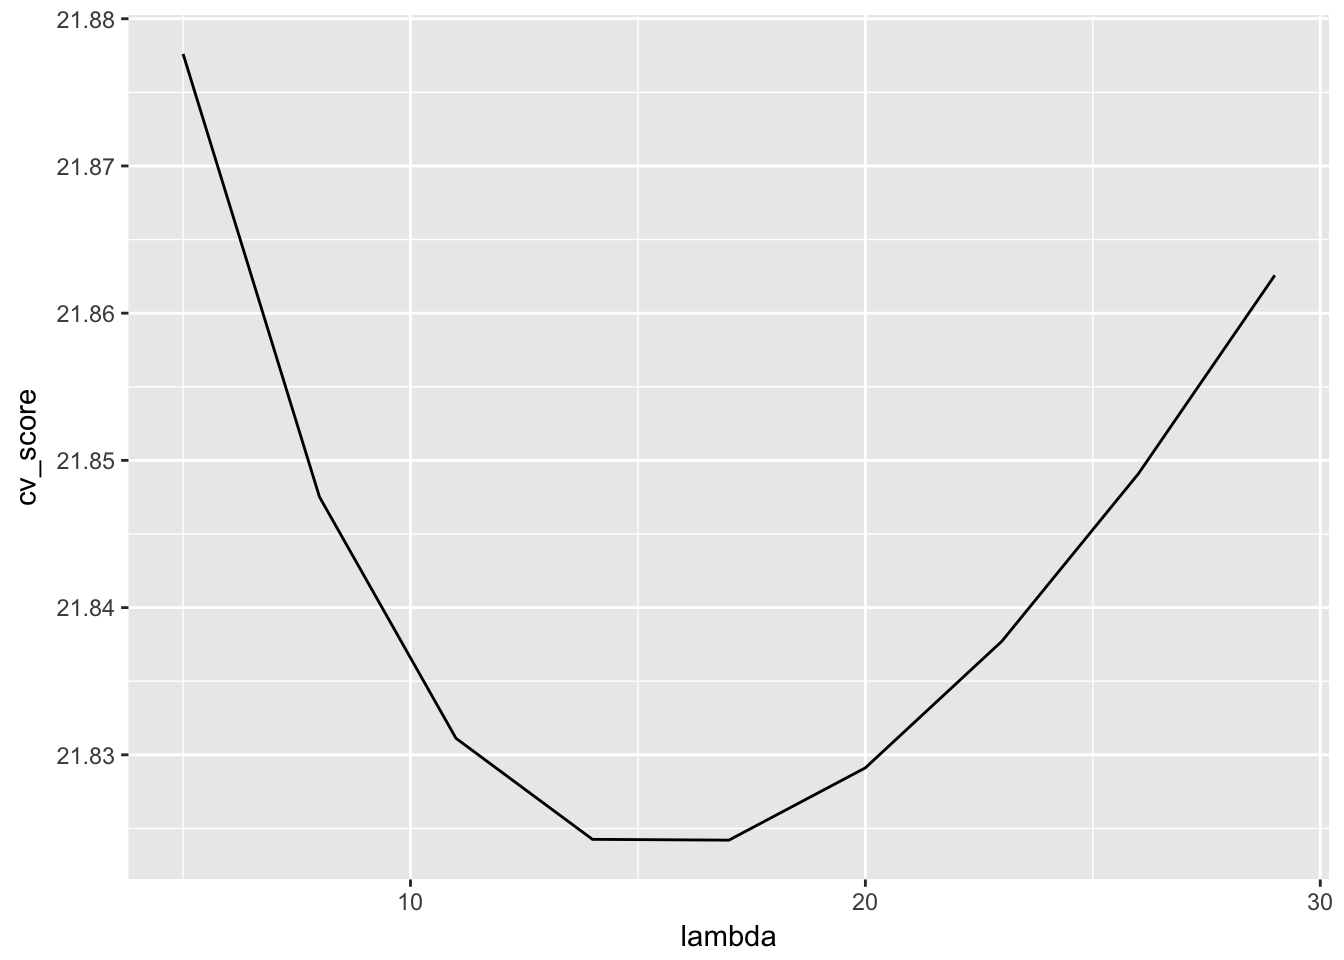
\includegraphics{comp_stats_summary_files/figure-latex/unnamed-chunk-19-1.pdf}

\begin{Shaded}
\begin{Highlighting}[]
\KeywordTok{summary}\NormalTok{(fitted$nk3) }
\end{Highlighting}
\end{Shaded}

\begin{verbatim}
## Call: earth(formula=y~x, data=sim, nk=3)
## 
##             coefficients
## (Intercept)    1.1193329
## h(x-30)        0.5104456
## 
## Selected 2 of 3 terms, and 1 of 1 predictors
## Termination condition: Reached nk 3
## Importance: x
## Number of terms at each degree of interaction: 1 1 (additive model)
## GCV 28.14687    RSS 3407.766    GRSq 0.8343005    RSq 0.8395191
\end{verbatim}

The example shows what we expected. The green line with a maximum of
three knots uses just one knot around 30, and only the right part of the
reflected pair is used. It cannot distinguish between the linear segment
between 40 and 75 and the sine-wave afterwards. By allowing more knots,
we can see that the red line fits the data quite well. Note that the
default of \texttt{degree} is just \(1\), so we don't have interaction
terms in the model. This does not matter for a one-dimensional example
anyways.

\section{Neural Networks}\label{neural-networks}

Neural networks are high-dimensional non-linear regression models. The
way it works is best illustrated with a picture.

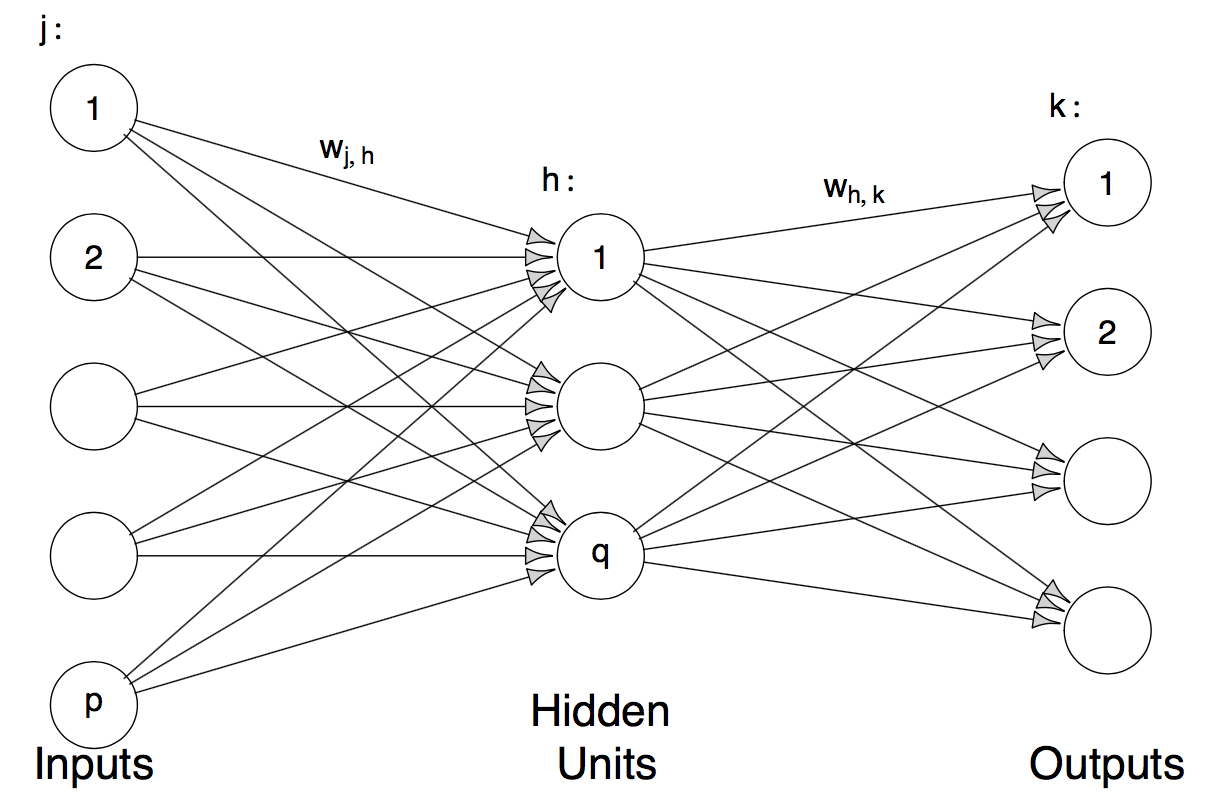
\includegraphics[width=16.81in]{figures/nn}

This is a neural network with one hidden layer, \(p\) input layers and
\(q\) output layers. Mathematically speaking, the model is:
\[ g_k(x) = f_0\Big(\alpha_k +
\sum\limits_{h = 1}^q w_{ij} \phi(\tilde{\alpha}_h + \sum\limits_{j = 1}^p
w_{jh}x_j)\Big)\] Where \(\phi(x)\) is the sigmoid function
\(\frac{exp(x)}{1 + exp(x)}\), \(f_0\) is the sigmoid function for
classification and the identity for regression. In the case of
regression \(k = 1\) is used, for classification we use
\(g_0, ..., g_{J-1}\) and then use the Bayes classifier
\(\mathcal{\hat{C}(x)} = \arg\max\limits_{0<j<J-1} g_j(x)\) (is that
correct?), which is called the softmax in the neural network literature.

\subsection{Fitting Neural Networks (in
R)}\label{fitting-neural-networks-in-r}

The \texttt{nnet} function from the package with the same name basically
uses gradient descent to maximize the likelihood. It is important to
first scale the data so the gradient descent does not get stuck in flat
regions of the sigmoid function.

\begin{Shaded}
\begin{Highlighting}[]
\KeywordTok{set.seed}\NormalTok{(}\DecValTok{22}\NormalTok{) }
\KeywordTok{data}\NormalTok{(}\StringTok{"ozone"}\NormalTok{, }\DataTypeTok{package =} \StringTok{"gss"}\NormalTok{) }
\KeywordTok{unloadNamespace}\NormalTok{(}\StringTok{"MASS"}\NormalTok{)}
\NormalTok{scaled <-}\StringTok{ }\NormalTok{ozone %>%}\StringTok{ }
\StringTok{  }\KeywordTok{select}\NormalTok{(-upo3) %>%}\StringTok{ }
\StringTok{  }\KeywordTok{scale}\NormalTok{() %>%}\StringTok{ }
\StringTok{  }\KeywordTok{as_data_frame}\NormalTok{() %>%}\StringTok{ }
\StringTok{  }\KeywordTok{mutate}\NormalTok{(}\DataTypeTok{log_upo3 =} \KeywordTok{log}\NormalTok{(ozone$upo3))}

\NormalTok{fit <-}\StringTok{ }\NormalTok{nnet::}\KeywordTok{nnet}\NormalTok{( log_upo3 ~., }\DataTypeTok{data =} \NormalTok{scaled, }
                   \DataTypeTok{size =} \DecValTok{3}\NormalTok{, }\CommentTok{# how many nodes in the *one* hidden layer. }
                   \DataTypeTok{decay =} \FloatTok{4e-4}\NormalTok{, }\CommentTok{# regularization. Multiply weights by 1 - decay after }
                   \CommentTok{# gradient step. }
                   \DataTypeTok{linout =} \OtherTok{TRUE}\NormalTok{, }\CommentTok{# linear output units (refers to f0?). }
                   \DataTypeTok{skip =} \OtherTok{TRUE}\NormalTok{, }\CommentTok{# add skip-layer connections between output and input. }
                   \DataTypeTok{maxit =} \DecValTok{500} \NormalTok{) }
\end{Highlighting}
\end{Shaded}

The weights between the nodes are:

\begin{Shaded}
\begin{Highlighting}[]
\KeywordTok{summary}\NormalTok{(fit) }
\end{Highlighting}
\end{Shaded}

\begin{verbatim}
## a 9-3-1 network with 43 weights
## options were - skip-layer connections  linear output units  decay=4e-04
##  b->h1 i1->h1 i2->h1 i3->h1 i4->h1 i5->h1 i6->h1 i7->h1 i8->h1 i9->h1 
##  -2.28   1.27  -0.34  -2.57   1.46   0.03   0.10  -1.02  -0.39  -0.33 
##  b->h2 i1->h2 i2->h2 i3->h2 i4->h2 i5->h2 i6->h2 i7->h2 i8->h2 i9->h2 
## -12.43   5.09   2.04   8.19  -7.66  -7.01   2.40  -0.31   3.59  -1.19 
##  b->h3 i1->h3 i2->h3 i3->h3 i4->h3 i5->h3 i6->h3 i7->h3 i8->h3 i9->h3 
## -19.77  -6.64   1.49  -4.53  -3.95   2.28   6.05   5.19  10.05  -0.20 
##   b->o  h1->o  h2->o  h3->o  i1->o  i2->o  i3->o  i4->o  i5->o  i6->o 
##   2.50  -1.81   0.68   0.71   0.11  -0.09  -0.49   0.72   0.01  -0.03 
##  i7->o  i8->o  i9->o 
##   0.04  -0.29  -0.15
\end{verbatim}

The in-sample MSE for the regression case is

\begin{Shaded}
\begin{Highlighting}[]
\KeywordTok{mean}\NormalTok{(}\KeywordTok{residuals}\NormalTok{(fit)^}\DecValTok{2}\NormalTok{) }
\end{Highlighting}
\end{Shaded}

\begin{verbatim}
## [1] 0.1036706
\end{verbatim}

\section{Projection Pursuit
Regression}\label{projection-pursuit-regression}

The model takes the form
\[g_{PPR} = \mu + \sum\limits_{k = 1}^q f_k(\sum \limits_{j = 1}^p
\alpha_{jk}x_j) \] With \(\sum \limits_{j = 1}^p \alpha_j = 1\) and
\(E[f_k(\sum \limits_{j = 1}^p \alpha_{jk}x_j)] = 0 \;\; \text{for all k}\).

\(\mathbf{\alpha}_k x_j\) is the projection of the j-th column in the
design matrix onto \(\alpha_k\). The functions \(f_k\) only vary along
one direction and are hence called ridge functions.

Projection pursuit regression is similar to both neural nets and
additive models. It is similar to GAMs because

\begin{itemize}
\tightlist
\item
  it can be seen as an additive model whereas the predictors were first
  projected into the optimal direction.
\end{itemize}

And it is similar neural nets because

\begin{itemize}
\tightlist
\item
  if you assume the identity for \(f_0\) in the neral net (which you
  typically do for regression) the models become very similar up to the
  term \(w_{hk} \phi\), which is just \(f_k\) in projection pursuit
  regression. Hence, instead of assuming a parapetric form (the sigmoid
  function) and multiplying that transformation with a weight
  \(w_{hk}\)\footnote{For regression you need only one index since you
    will have just one ouput layer.} we don't make any assumption on the
  form of the function, that is, let \(f_k\) be fully non-parametric.
\end{itemize}

Probably fot that very reason, the model requires much smaller \(q\)
than a neural net requires hidden units, at the expense of estimating
the ridge functions (which is not necessary for neural nets).

\subsection{Proejction Pursuit
Example}\label{proejction-pursuit-example}

In the following, we illustrate how optimal projections of the initial
predictor space can allow us to use an additive functional form to deal
with interaction terms. Let us consider the following data-generating
model
\[ Y = X_1 \times X_2 + \epsilon \; \text{with} \;\epsilon \sim N(0, 1) \; \text{and}\; X_1, X_2 \sim \text{Unif}(-1,1)\]

Where \(X \in \mathbb{R}^2\), i.e.~a two-dimensional predictor space
with the predictors \(X_1\) and \(X_2\). Using elementary calculus, this
can be rewritten as
\[ Y = \frac{1}{4} (X_1 + X_2)^2  - \frac{1}{4}(X_1 - X_2)^2\] Hence, we
rewrote a multiplicative model as an additive model. As we are using
arbitrary \emph{smooth} functions \(f_k\), we can easily fit the
quadratic terms in the equation above, so the problem to solve becomes
\[Y = \mu + f_1(X_1 + X_2) - f_2(X_1 - X_2)\] Therefore, the remaining
question is how can we choose the two vectors \(\mathbf{\alpha}_1\) and
\(\mathbf{\alpha}_1\) such that the result of the projection is
\(X_1 + X_2 \;\text{and}\;X_1 - X_2\). With the restriction
\(|\alpha| = 1\), it turns out we can proceed as follows: We project the
first predictor onto \((\alpha_{11}, \alpha_{12}) = (0.7, 0.7)\) and the
second predictor onto \((\alpha_{11}, \alpha_{12}) = (0.7, -0.7)\). This
yields \(0.7(X_1 + X_2)\) and \(0.7(X_1 - X_2)\).

Let's implement that with R

\begin{Shaded}
\begin{Highlighting}[]
\NormalTok{data <-}\StringTok{ }\KeywordTok{data_frame}\NormalTok{(}
  \DataTypeTok{x1 =} \KeywordTok{runif}\NormalTok{(}\DecValTok{500}\NormalTok{, -}\DecValTok{1}\NormalTok{, }\DecValTok{1}\NormalTok{),}
  \DataTypeTok{x2 =} \KeywordTok{runif}\NormalTok{(}\DecValTok{500}\NormalTok{, -}\DecValTok{1}\NormalTok{, }\DecValTok{1}\NormalTok{),}
  \DataTypeTok{y =} \NormalTok{x1*x2 +}\StringTok{ }\KeywordTok{rnorm}\NormalTok{(}\DecValTok{500}\NormalTok{, }\DecValTok{0}\NormalTok{, }\FloatTok{0.005}\NormalTok{)}
\NormalTok{)}
\NormalTok{all <-}\StringTok{ }\KeywordTok{ggplot}\NormalTok{(data, }\KeywordTok{aes}\NormalTok{(}\DataTypeTok{x =} \NormalTok{x1, }\DataTypeTok{y =} \NormalTok{x2)) +}\StringTok{ }
\StringTok{  }\KeywordTok{geom_point}\NormalTok{(}\KeywordTok{aes}\NormalTok{(}\DataTypeTok{color =} \NormalTok{y), }\DataTypeTok{size =} \DecValTok{3}\NormalTok{) +}\StringTok{ }
\StringTok{  }\KeywordTok{scale_color_gradient2}\NormalTok{()}
\end{Highlighting}
\end{Shaded}

We can see the obvious pattern, but we can also see that an additive
model would not do well on that.

\begin{Shaded}
\begin{Highlighting}[]
\NormalTok{x1y <-}\StringTok{ }\KeywordTok{ggplot}\NormalTok{(data, }\KeywordTok{aes}\NormalTok{(}\DataTypeTok{x =} \NormalTok{x1, }\DataTypeTok{y =} \NormalTok{y)) +}\StringTok{ }
\StringTok{  }\KeywordTok{geom_point}\NormalTok{(}\KeywordTok{aes}\NormalTok{(}\DataTypeTok{color =} \NormalTok{y), }\DataTypeTok{size =} \DecValTok{3}\NormalTok{) +}\StringTok{ }
\StringTok{  }\KeywordTok{geom_smooth}\NormalTok{() +}\StringTok{ }
\StringTok{  }\KeywordTok{scale_color_gradient2}\NormalTok{()}


\KeywordTok{grid.arrange}\NormalTok{(all, x1y)}
\end{Highlighting}
\end{Shaded}

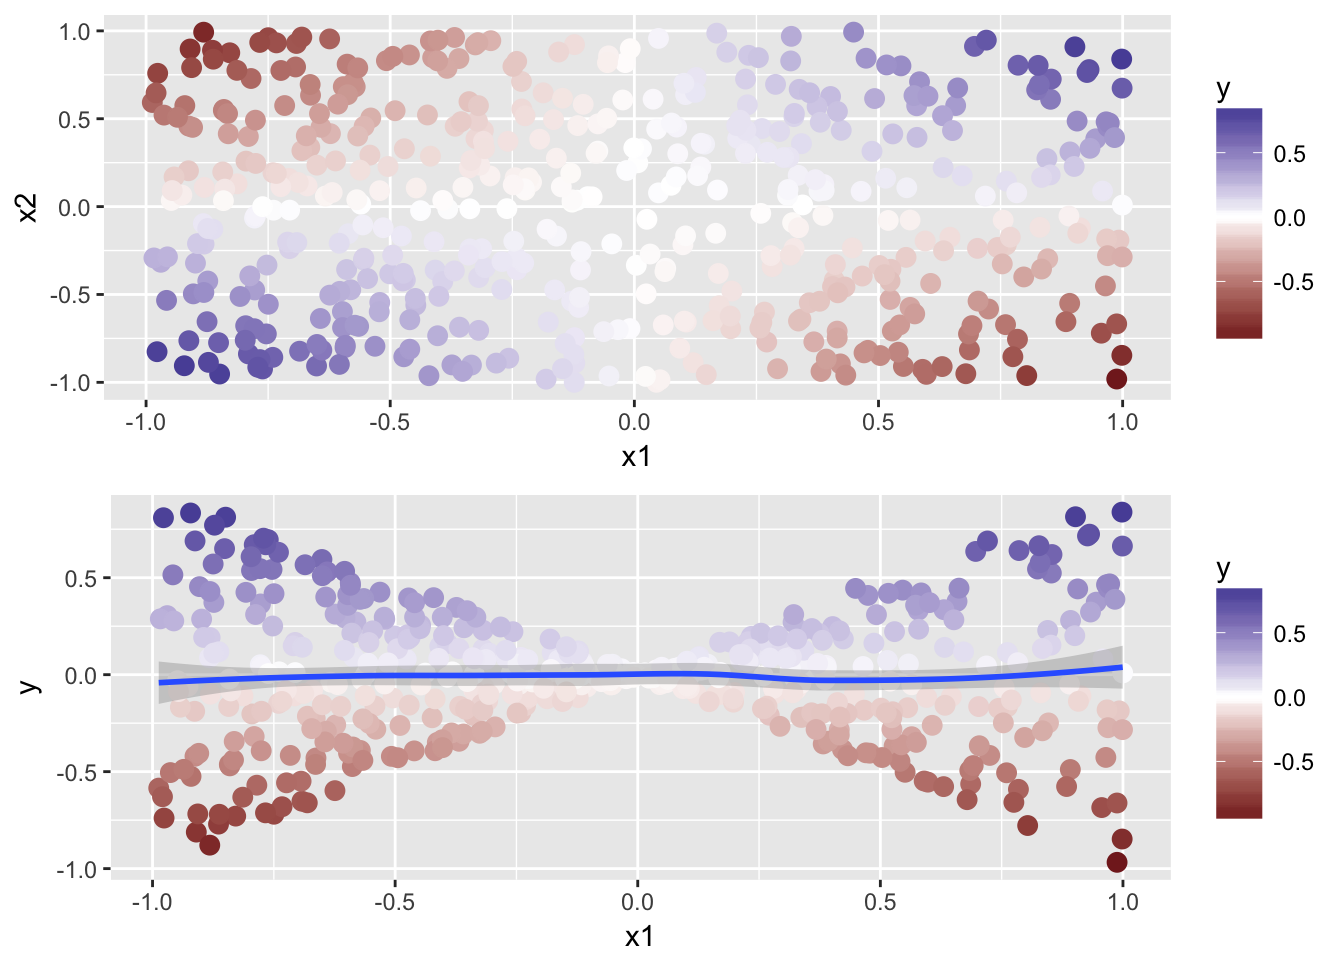
\includegraphics{comp_stats_summary_files/figure-latex/unnamed-chunk-25-1.pdf}

How about using the aforementioned projection?

\begin{Shaded}
\begin{Highlighting}[]
\NormalTok{data <-}\StringTok{ }\NormalTok{data %>%}
\StringTok{  }\KeywordTok{mutate}\NormalTok{(}
    \DataTypeTok{projected_x1 =} \FloatTok{0.7}\NormalTok{*(x1 +}\StringTok{ }\NormalTok{x2),}
    \DataTypeTok{projected_x2 =} \NormalTok{-}\FloatTok{0.7}\NormalTok{*(x1 -}\StringTok{ }\NormalTok{x2)}
  \NormalTok{)}

\NormalTok{projected_all <-}\StringTok{ }\KeywordTok{ggplot}\NormalTok{(data, }\KeywordTok{aes}\NormalTok{(}\DataTypeTok{x =} \NormalTok{projected_x1, }\DataTypeTok{y =} \NormalTok{projected_x2)) +}\StringTok{ }
\StringTok{  }\KeywordTok{geom_point}\NormalTok{(}\KeywordTok{aes}\NormalTok{(}\DataTypeTok{color =} \NormalTok{y), }\DataTypeTok{size =} \DecValTok{3}\NormalTok{) +}\StringTok{ }
\StringTok{  }\KeywordTok{scale_color_gradient2}\NormalTok{()}

\NormalTok{projected_x1 <-}\StringTok{ }\KeywordTok{ggplot}\NormalTok{(data, }\KeywordTok{aes}\NormalTok{(}\DataTypeTok{x =} \NormalTok{projected_x1, }\DataTypeTok{y =} \NormalTok{y)) +}\StringTok{ }
\StringTok{  }\KeywordTok{geom_point}\NormalTok{(}\KeywordTok{aes}\NormalTok{(}\DataTypeTok{color =} \NormalTok{y), }\DataTypeTok{size =} \DecValTok{3}\NormalTok{) +}\StringTok{ }
\StringTok{  }\KeywordTok{geom_smooth}\NormalTok{() +}\StringTok{ }
\StringTok{  }\KeywordTok{scale_color_gradient2}\NormalTok{()}

\NormalTok{projected_x2 <-}\StringTok{ }\KeywordTok{ggplot}\NormalTok{(data, }\KeywordTok{aes}\NormalTok{(}\DataTypeTok{x =} \NormalTok{projected_x2, }\DataTypeTok{y =} \NormalTok{y)) +}\StringTok{ }
\StringTok{  }\KeywordTok{geom_point}\NormalTok{(}\KeywordTok{aes}\NormalTok{(}\DataTypeTok{color =} \NormalTok{y), }\DataTypeTok{size =} \DecValTok{3}\NormalTok{) +}\StringTok{ }
\StringTok{  }\KeywordTok{geom_smooth}\NormalTok{() +}\StringTok{ }
\StringTok{  }\KeywordTok{scale_color_gradient2}\NormalTok{()}

\NormalTok{fitted_x1 <-}\StringTok{ }\NormalTok{mgcv::}\KeywordTok{gam}\NormalTok{(y~}\KeywordTok{s}\NormalTok{(projected_x1), }\DataTypeTok{data =} \NormalTok{data)}
\NormalTok{fitted_x2 <-}\StringTok{ }\NormalTok{mgcv::}\KeywordTok{gam}\NormalTok{(y~}\KeywordTok{s}\NormalTok{(projected_x2), }\DataTypeTok{data =} \NormalTok{data)}

\NormalTok{data <-}\StringTok{ }\NormalTok{data %>%}
\StringTok{  }\KeywordTok{mutate}\NormalTok{(}\DataTypeTok{fitted =} \KeywordTok{predict}\NormalTok{(fitted_x1) +}\StringTok{ }\KeywordTok{predict}\NormalTok{(fitted_x2))}

\NormalTok{fitted <-}\StringTok{ }\KeywordTok{ggplot}\NormalTok{(data, }\KeywordTok{aes}\NormalTok{(}\DataTypeTok{x =} \NormalTok{x1, }\DataTypeTok{y =} \NormalTok{x2)) +}\StringTok{ }
\StringTok{  }\KeywordTok{geom_point}\NormalTok{(}\KeywordTok{aes}\NormalTok{(}\DataTypeTok{color =} \NormalTok{fitted), }\DataTypeTok{size =} \DecValTok{3}\NormalTok{) +}\StringTok{ }
\StringTok{  }\KeywordTok{scale_color_gradient2}\NormalTok{()}
\KeywordTok{grid.arrange}\NormalTok{(projected_all, projected_x1, projected_x2, fitted, }\DataTypeTok{nrow =} \DecValTok{2}\NormalTok{)}
\end{Highlighting}
\end{Shaded}

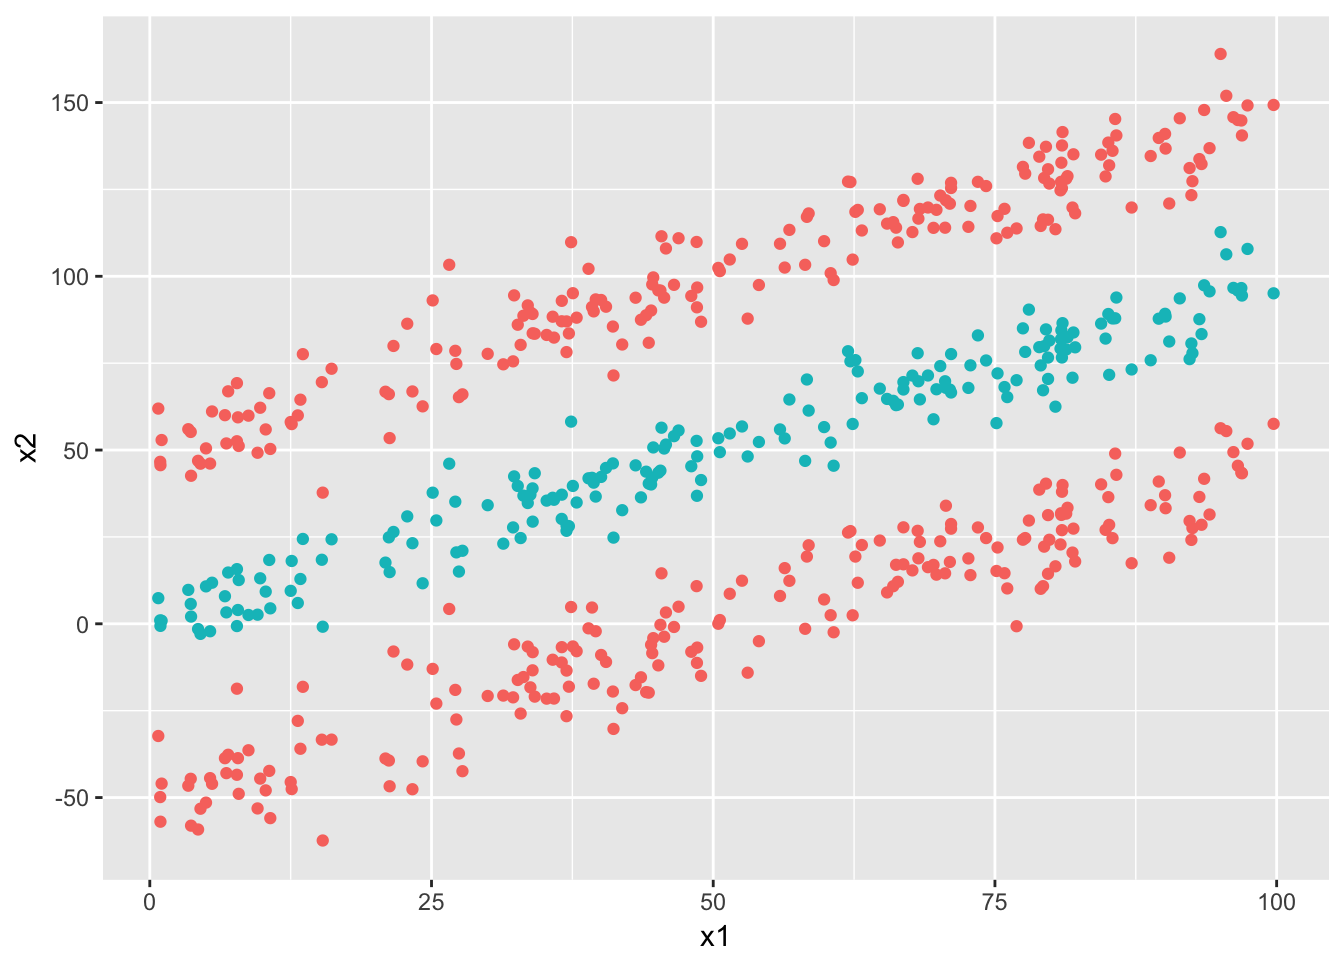
\includegraphics{comp_stats_summary_files/figure-latex/unnamed-chunk-26-1.pdf}

The bottom right picture shows the predictions with the projection
pursuit approach, which resembles the original data pretty well. Again,
the idea is to use an additive model to account for the interactions
properly by first projecting the predictors optimally.

\section{Classification and Regression
Trees}\label{classification-and-regression-trees}

The model function for trees is
\[g_{tree}(x) = \sum\limits_{r = 1}^M \beta_r1_{[x \in \mathcal{P}_r]}\]
Where \(\mathcal{P} = \cup_{j = 1}^M \mathcal{P}_j\), that is, the space
\(\mathcal{P} \in \mathbb{R}^p\) is devided into \(M\) disjoint
partitions. Hence, note that in the sum above, \(x\) can only be in one
of the \(M\) martitions and hence, all but one indicator functions are
zero in the sum. The model yields a \textbf{pice-wise constant}
response, that is, the prediction is the same for all
\(x \in \mathcal{P}_r\). That can be visualized nicely in a
two-dimensional predictor space.

\begin{figure}
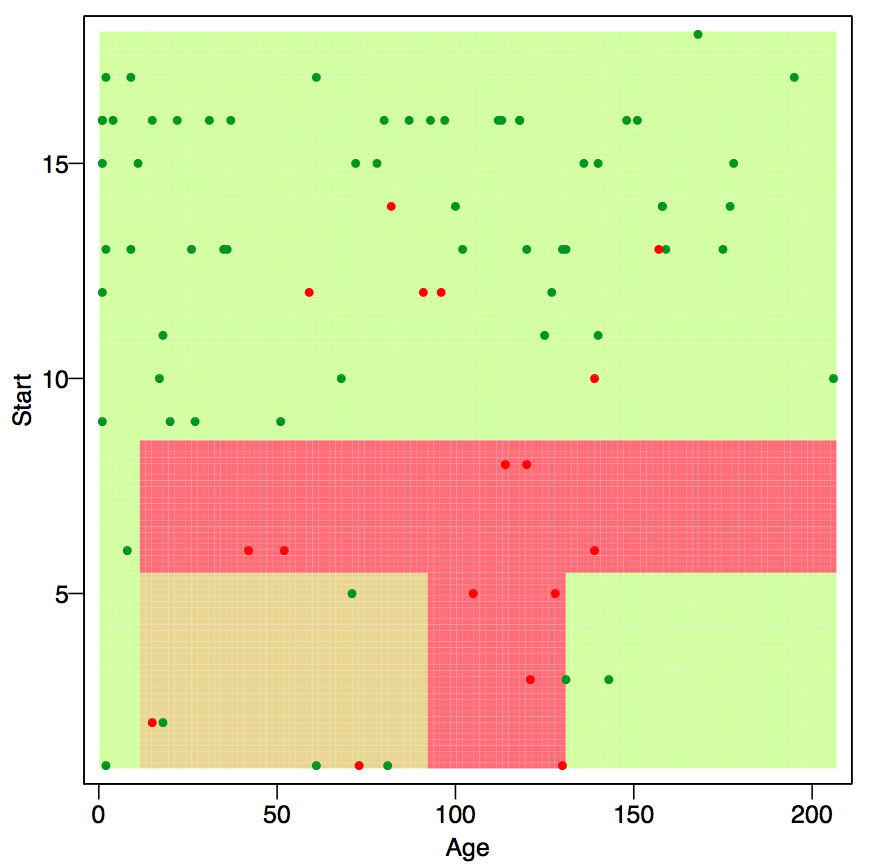
\includegraphics[width=12.15in]{figures/tree-partitioning} \caption{Partition with `rpart()`. Color indicate result of the majority voting Source: course script p. 73.}\label{fig:treepart}
\end{figure}

Trees are similar to multivariate adaptive regression splines MARS, as
mentioned in section \ref{mars} in the sense that they allow for
interaction effects. This can be seen well in figure \ref{fig:treepart}.
Going form age 50 to age 100 has different effects depending on the
start. Trees are different from MARS as they are piece-wise constant,
whereas MARS are pice-wise linear.

\subsection{Prediction given
Partitioning}\label{prediction-given-partitioning}

Estimation of the parameters \(\beta_1, ..., \beta_M\) is easy if the
partitioning is known. For Regression, it is simply the average of the
response variables for the subset of the data that lays within the
partition. Mathematically speaking
\[ \hat{\beta}_r = \sum\limits_{i = 1}^n 1_{[x_i \in \mathcal{P}_r]} Y_i / 
\sum\limits_{i = 1}^n 1_{[x_i \in \mathcal{P}_r]}\]

For classification, the class of a partition \mathcal{P}\_j is
determined by the largest group within that partition). We can estimate
the class probabilities directly (also for J \textgreater{} 2) for the
r-th partition as follows:

\[ \hat{\pi}_j(x) =
\frac{\# \text{from class j in}\; \mathcal{P}_r}{\#\text{total in}\; \mathcal{P}_r} = 
\sum\limits_{i = 1}^n 1_{[Y_i = j]} 
1_{[x_i \in \mathcal{P}_r]}/ 
\sum\limits_{i = 1}^n 1_{[x_i \in \mathcal{P}_r]}\]

\subsection{Assumptions on the
Patritions}\label{assumptions-on-the-patritions}

As we saw above, obtaining predictions \emph{given} the partitioning is
not hard. The more difficult problem is to obtain the partitions. By
imposing some restrictions on the shape of the partitions and the
strategy to choose them, we can limit the complexity of the question at
hand. Namely, we

\begin{itemize}
\tightlist
\item
  assume partitions that are \textbf{axes parallel rectangles}, just as
  depicted in the pictuer above. Note that this is a stronger limitation
  than just assuming linear (decision) boundaries since these boundaries
  also need to be parallel to the axis. For example, decision trees
  would not do well on a classification problem like this (unless there
  is a lot of data and we can have many splits:
\end{itemize}

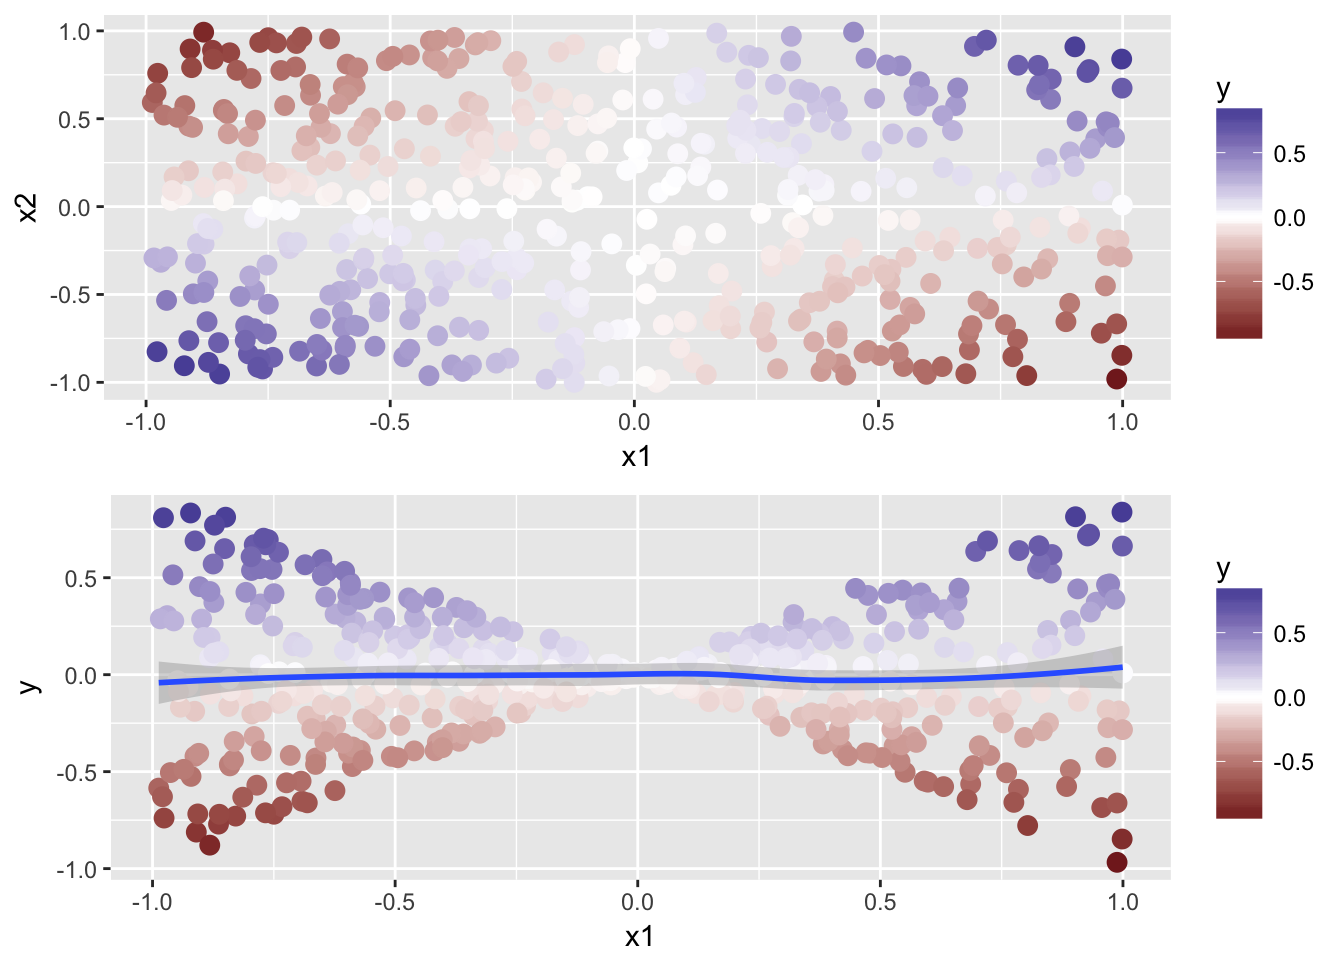
\includegraphics{comp_stats_summary_files/figure-latex/unnamed-chunk-28-1.pdf}

\begin{itemize}
\tightlist
\item
  we use a \textbf{greedy} algorithm since the space of possible
  partitioning schemes is still huge.
\end{itemize}

\subsection{Algorithm}\label{algorithm}

The algorithm now looks as follows:

\begin{enumerate}
\def\labelenumi{\arabic{enumi}.}
\tightlist
\item
  Start with \(M = 1\) and
  \(\mathcal{P} = \{\mathcal{R}\} = \mathbb{R}^p\).
\item
  Redefine \(\mathcal{R}\) as
  \(\mathcal{R_{left}} \cup \mathcal{R_{right}}\) where
\end{enumerate}

\(\mathcal{R}_{left} \;= \mathbb{R}\times\mathbb{R}\;...\; \times(-\infty, d]\times  \mathbb{R} ...\times\mathbb{R}\)

\(\mathcal{R}_{right} = \mathbb{R}\times\mathbb{R}\;...\; \times(d, \infty)\times  \mathbb{R} ...\times\mathbb{R}\)

where \(d\) is a value from the \emph{finite} set of midpoints between
the data points with regard to the dimension currently considered. We
search over all dimensions \(j \in \{1, ..., p\}\) and within each
dimension over all potential split points \(d\) such that the negative
log-likelihood is decreased the most. The new partition is
\(\mathcal{P} = \{R_{left}, R_{right}\}\)

\begin{enumerate}
\def\labelenumi{\arabic{enumi}.}
\setcounter{enumi}{2}
\tightlist
\item
  We again refine the current partition as in step 2 by splitting up
  \emph{one} partition into two parts. Then, we update the partition
  \[\mathcal{P} = \mathcal{P}_{old} \setminus \mathcal{P}_{to\;refine} \;\cup\{R_{left}, R_{right}\} \]
\item
  Iterate over the step 3 \(M\) times.
\item
  Prune the tree by reverting some of the partitioning steps above until
  the optimal size of the tree is found (e.g via cross-validation).
\end{enumerate}

You can fit a tree in R with the \texttt{rpart} package, which stands
for recursive partitioning.

\begin{Shaded}
\begin{Highlighting}[]
\NormalTok{tree <-}\StringTok{ }\NormalTok{rpart::}\KeywordTok{rpart}\NormalTok{(}
  \NormalTok{upo3~., }
  \DataTypeTok{data =} \NormalTok{ozone,}
  \DataTypeTok{control =} \KeywordTok{list}\NormalTok{(}
    \DataTypeTok{minsplit =} \DecValTok{20}\NormalTok{,}
    \DataTypeTok{cp =} \FloatTok{0.003}
  \NormalTok{)}
\NormalTok{)}
\end{Highlighting}
\end{Shaded}

\subsection{Backward Deletion /
Pruning}\label{backward-deletion-pruning}

After \(M\) steps, there will be \(M + 1\) partitions. This can also be
visualized nicely in a tree structure.

\begin{Shaded}
\begin{Highlighting}[]
\NormalTok{rpart::}\KeywordTok{prune}\NormalTok{(tree, }\DataTypeTok{cp =} \FloatTok{0.05}\NormalTok{) %>%}\StringTok{ }\CommentTok{# prune tree for illustrative purposes}
\NormalTok{rpart.plot::}\KeywordTok{prp}\NormalTok{(}\DataTypeTok{extra =} \DecValTok{1}\NormalTok{,}
    \DataTypeTok{box.col=}\KeywordTok{c}\NormalTok{(}\StringTok{'pink'}\NormalTok{, }\StringTok{'palegreen3'}\NormalTok{, }\StringTok{'lightsteelblue 2'}\NormalTok{,}\StringTok{'lightgoldenrod 1'}\NormalTok{)[tree$frame$yval])}
\end{Highlighting}
\end{Shaded}

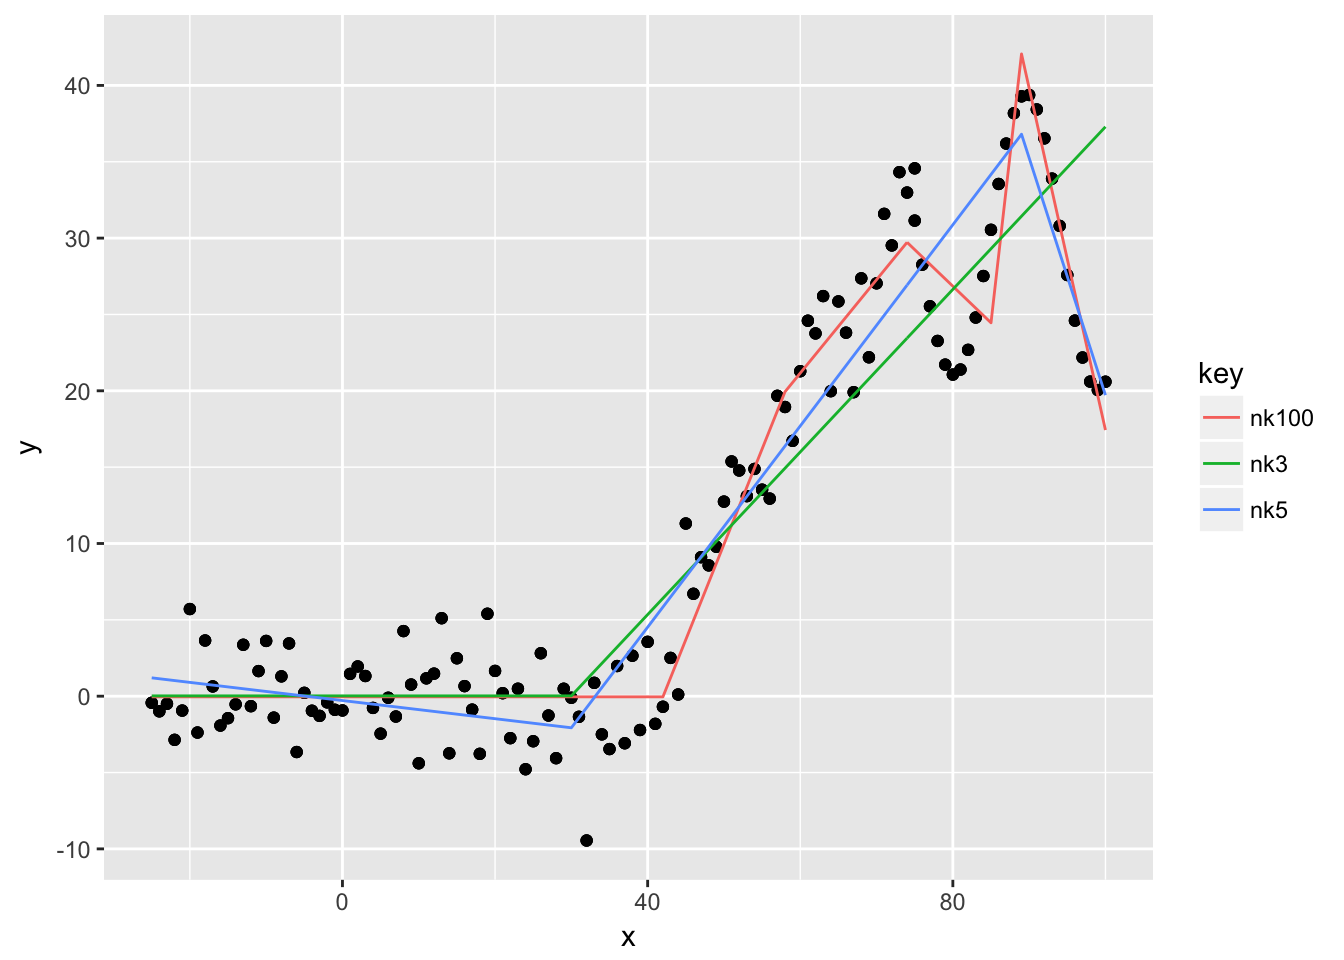
\includegraphics[width=650px]{comp_stats_summary_files/figure-latex/unnamed-chunk-30-1}

The idea is now to subsequently remove the leaves from the tree such
that the negative log-likeihood increases the least. If we do that until
no leaf is left, we end up with a sequence of trees.

\begin{equation}
\mathcal{T}_M \supset \mathcal{T}_{M-1} \;\;...\;\;\supset \mathcal{T}_{\emptyset}
\label{eq:treeset}
\end{equation}

Just as with Mallow's \(C_p\), we can compute a score for every model
that is increasing in the fit of the model but also has a complexity
penality

\[R_{\alpha}(\mathcal{T}) = R(\mathcal{T}) + \alpha \times \text{size}(\mathcal{T})\]

Now, we only need to find the right alpha. We can set a few alpha
values, then find the best tree for this alpha
\(\mathcal{T}(\alpha) = \arg\min\limits_{\mathcal{T} \subset \mathcal{T}_M}R_{\alpha}(\mathcal{T})\)
and then do cross-validation for these alpha values to find the optimal
alpha. It can be shown that the set
\(\{\mathcal{T}(\alpha)| \alpha \in (0, \infty]\}\) is \emph{nested} and
the same or a subeset of the set in equation \eqref{eq:treeset}. Use
\texttt{rpart::plotcp()} to plot the size of the optimal trees for each
alpha against the cross-validation score. Then, use the one-standard
error rule to select the idal tree size. That is first find the tree
with the lowest relative error. Then add one standard error to it's
error and find the smallest tree that does not execced this relative
error. The idea behind this approach is to choose good model that
performs similar to the best (and potentially complex) model but is as
simple as possible.

\begin{Shaded}
\begin{Highlighting}[]
\NormalTok{rpart::}\KeywordTok{plotcp}\NormalTok{(tree)}
\end{Highlighting}
\end{Shaded}

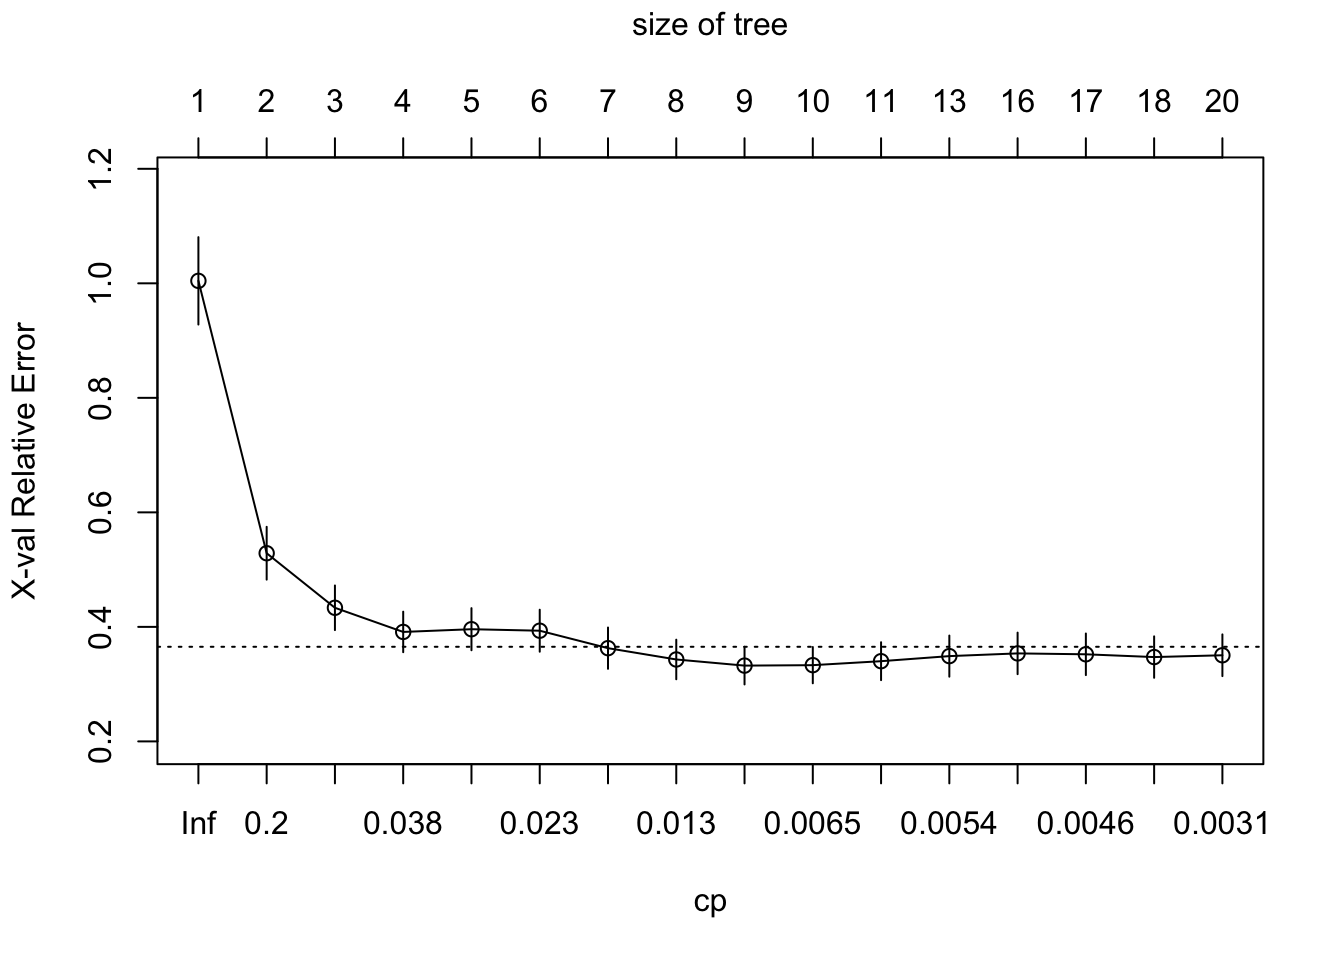
\includegraphics[width=650px]{comp_stats_summary_files/figure-latex/unnamed-chunk-31-1}

\subsection{Pros and Cons of Trees}\label{pros-and-cons-of-trees}

Pros are:

\begin{itemize}
\tightlist
\item
  Straightforward interpretation. Show it your grand mother and she will
  understand it.
\item
  Allow for interaction effects.
\item
  Competitive performance.
\item
  Can deal with missing values thanks to the \emph{surrogate split}. For
  each node the tree algorithm tries to find variables that are highly
  correlated with the selected splitter. Then, if this variable is not
  available for a new observation to be classified, the surrogate is
  used to classifiy the observation on that split node so subsequent
  nodes can further process the observation.
\item
  The variable selection is done automatically and variables that are
  higher up in the hierarchy are considered to be more imporatant for
  prediction. We will have a look at ridge regression and LASSO which
  also do variable selection automatically, but the feature is not
  present in any method we looked at before.
\end{itemize}

There are some cons also:

\begin{itemize}
\tightlist
\item
  First and foremost, trees yield \textbf{piece-wise} constant
  predictions, which is typically not what we assume the true
  underlaying function to look like.
\item
  Subsequent splits depend on previous splits. Therefore, if an early
  split is \emph{wrong}, everything following afterwards is
  \emph{wrong}. This means the algorithm may not be very stable.
\end{itemize}

? question how would you use mars for classification?

\subsection{Random Forests}\label{random-forests}

Random forests are made up of three main ingredients:

\begin{itemize}
\tightlist
\item
  regression (or classification) trees
\item
  boostrapping
\item
  aggregating
\end{itemize}

The algorithm is as follows:

\begin{itemize}
\tightlist
\item
  draw \(n_{tree}\) boostrap samples (of size n obviously).
\item
  build for each of them an \emph{unpruned} tree. However, instead of
  searching over all \(p\) variables for the best split at each node,
  just consider a random sample of \(m_{try}\) variables for the split
  at each node. Obviously, \(m_{try} = p\) is the tree solution
  introduced before and corresponds to the bagging (which stands for
  boostrap aggregating, introduced later).
\item
  Predict a new data point by aggregating the \(n_{tree}\) prediction
  (majority vote for classification, averaging for regression).
\end{itemize}

To obtain an estimate for the generalization error, you can use the
\textbf{out-of-bag} approach, that is

\begin{itemize}
\tightlist
\item
  At each boostrap iteration, make predictions with the data that is not
  in the boostrap sample.
\item
  aggregate the predictions for all \(n_{tree}\) trees and compute the
  error rate and call it \emph{out-of-bag estimate of the error rate}.
\end{itemize}

The only drawback of trees is that interpretability is lower than for
trees.

\chapter{Variable Selection - Ridge Regression an
Lasso}\label{variable-selection---ridge-regression-an-lasso}

Except for trees, none of the techniques introduced so far perform
variable selection. Variable selection is particularly important when
working with high-dimensional data, namely for two reasons:

\begin{itemize}
\tightlist
\item
  In the case of highly correlated predictors, regression coefficient
  estimates become \textbf{ill-determined}, which means - loosly
  speaking - that there are a lot of different values for each predictor
  such that the model leads to the same prediction if the other
  coefficients are set wisely. This is undesirable. Note that the fitted
  values are not ill-determined since they don't vary when changing the
  coefficients.
\item
  In cases where we have \textbf{\(\mathbf{n}> \mathbf{p}\)}, we cannot
  estimate many models, so for example OLS. That means we first need to
  select some predictors before we can proceed.
\end{itemize}

In addition, a model with few predictors is often easier to interpret
than a model with many predictors.

\textbf{Ride and Lasso - which is which?} Ridge regression - two words,
is the method with an L2-penalty. Lasso is just one word - and has an
L1-penalty.

\section{Ridge Regression}\label{ridge-regression}

Consider the OLS Problem
\[y_i = \beta_0 + \beta_1 x_1 + \beta_2 x_2 + ... + \beta_p x_p +  \epsilon\]
We can demean the predictors and obtain
\[y_i = \beta_0 + \beta_1(x_1 - \bar{x}_1) + \beta_2(x_2 - \bar{x}_2) + ... 
+ \beta_p(x_p - \bar{x}_p) + \epsilon\] In which case
\(\hat{\beta}_0 = \bar{Y} - \hat{\beta}_1\bar{X} = \bar{Y}\) and can
take it to the other side and end up with the model.
\[\tilde{y} = \hat{\beta}_1 \tilde{x}_1 + \hat{\beta}_2 \tilde{x}_2 + 
... \hat{\beta}_p \tilde{x}_p +\epsilon\]

With all variables having a mean of zero. Hence we got rid of the
intercept. In order to compare the different \(\beta\)s, we should also
scale the predictors. Hence, if there are two variables that are highly
correlated, we can expres this part of the model equation as follows
\[ \beta_j x^{(j)} + \beta_k x^{(k)} \approx (\beta_j + c \beta_j ) x^{(j)}\]
You can see that for each \(\beta_j\), we can find an appropriate
\(\beta_k\) so that the sum does not change. That's what we meant above
when we said the coefficients are not stable but the sum is. One way to
make the coefficients \emph{better-determined} is to impose further
conditions on them. For example, we can restrict
\(\sum\limits_{j = 1}^p \beta_j < s\). The regression problem becomes
\[\beta = \arg\min\limits_{\|\beta\| < s}\|X\beta\|\] which is
equivalent to the lagrangian problem
\(\arg\min\limits_{\beta} \{ \|X \beta \|+ \lambda \| \beta \|_2^2 \}\)
With a one-to-one mapping of \(s \rightarrow \lambda\) Note that this is
a generalization of the least square solution since it contains the
least squares solution for \(\lambda = 0\). The resulting normal
equations are \[(X'X + \lambda I)^{-1}\hat{\beta}^* = X'Y\] Where one
can see that the matrix to invert will be non-singular \(\lambda > 0\),
even if \(X'X\) is singular. Due to this shrinking, it is intuitive that
the \(E[\hat{\beta}] \neq \beta\), that is, the coefficient will be
biased. That can be seen easily if we \emph{sneak in} the ols solution
for which we know it is unbiased.

\begin{equation}
\begin{split}

(E[\hat{\beta}] = & E[(X'X + \lambda I)^{-1}X'y]) \\
& E[(X'X + \lambda I)^{-1} (X'X)(X'X)^{-1}X'y] \\
& E[(X'X + \lambda I)^{-1} (X'X)\beta^{ols}] \\
& (X'X + \lambda I)^{-1} (X'X)\beta^{ols}
\end{split}
\end{equation}

Whereas \(E[\hat{\beta}] \neq \beta\) for \(\lambda > 0\) Also, we can
see that for \(\lambda \rightarrow \infty\), \(\beta \rightarrow 0\).

However, since by introducing a bias, we at the same time decrease the
variance of our estimator. Therefore, we can optimize the bias-variance
trade-off by finding an appropriate \(\lambda\), e.g.~by (generalized)
cross-valdiation. The regularization parameter lamda here is similar to
the one we saw in the chapter about smoothing splines.

To estimate the model, we can use the \texttt{MASS} package.

\begin{Shaded}
\begin{Highlighting}[]
\NormalTok{fitted <-}\StringTok{ }\NormalTok{MASS::}\KeywordTok{lm.ridge}\NormalTok{(}
  \NormalTok{GNP.deflator ~., }
  \CommentTok{# it's lamBda, not lamda! R won't complain due to ... !}
  \DataTypeTok{lambda =} \KeywordTok{seq}\NormalTok{(}\DecValTok{0}\NormalTok{, }\FloatTok{0.1}\NormalTok{, }\DataTypeTok{by =} \FloatTok{0.001}\NormalTok{), }
  \DataTypeTok{data =} \NormalTok{longley}
\NormalTok{)}
\end{Highlighting}
\end{Shaded}

We can plot the coefficients for different values of \(\lambda\) in a
so-called trace plot.

\begin{Shaded}
\begin{Highlighting}[]
\KeywordTok{plot}\NormalTok{(fitted)}
\end{Highlighting}
\end{Shaded}

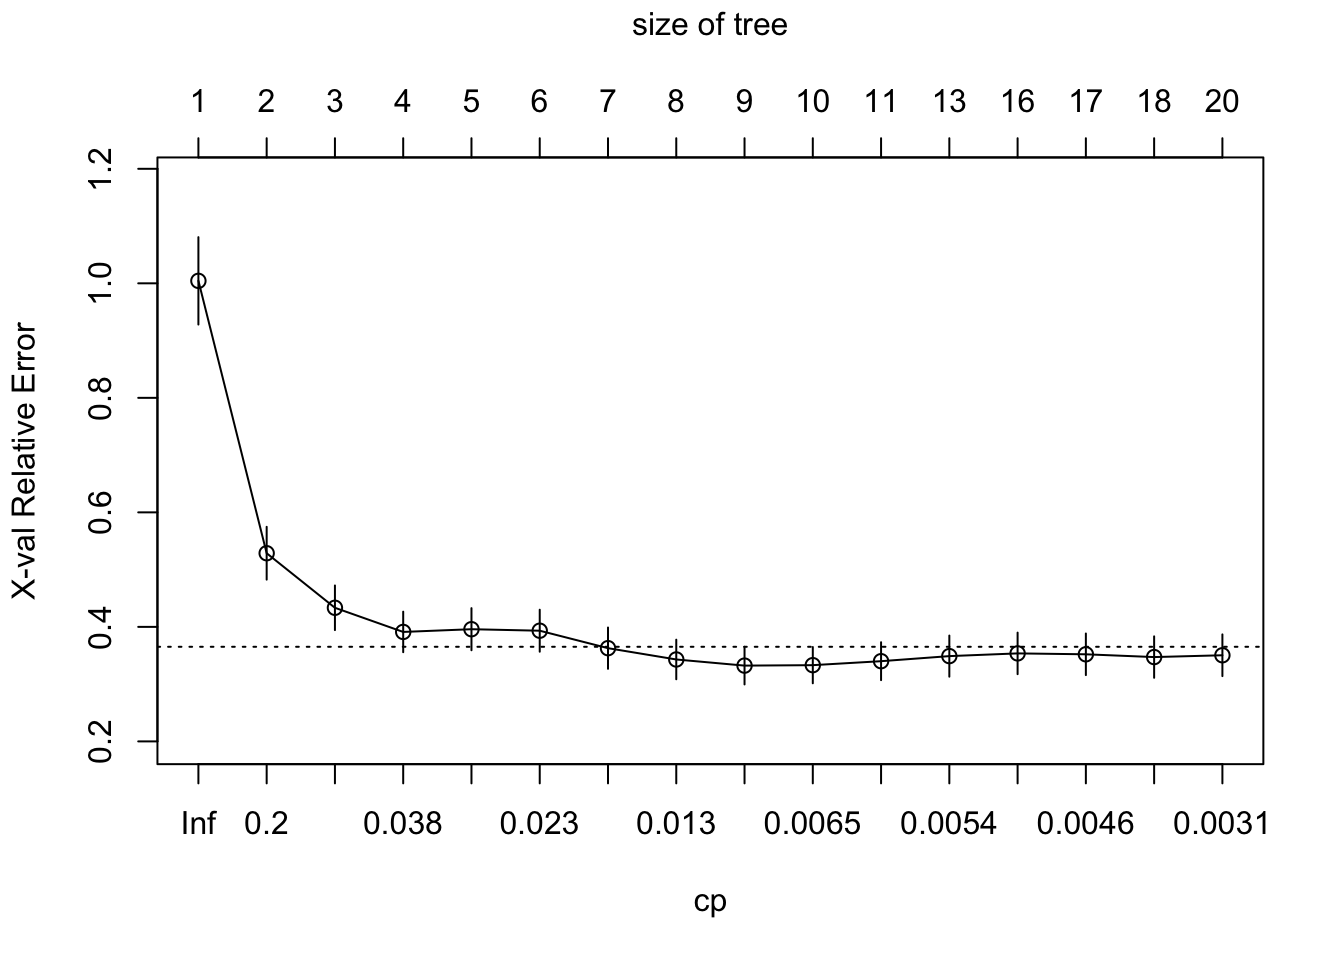
\includegraphics{comp_stats_summary_files/figure-latex/unnamed-chunk-33-1.pdf}

We can also get the coeficients for each lamda we estimated and select
the best model and get the usual \texttt{lm} summary for it.

\begin{Shaded}
\begin{Highlighting}[]
\KeywordTok{coef}\NormalTok{(fitted) %>%}
\StringTok{  }\KeywordTok{as_data_frame}\NormalTok{()}
\end{Highlighting}
\end{Shaded}

\begin{verbatim}
## # A tibble: 101 x 7
##            ``       GNP Unemployed Armed.Forces Population        Year
##         <dbl>     <dbl>      <dbl>        <dbl>      <dbl>       <dbl>
##  1 2946.85636 0.2635272 0.03648291  0.011161050  -1.737030 -1.41879853
##  2 1895.97527 0.2392348 0.03100610  0.009372158  -1.643803 -0.87657471
##  3 1166.33337 0.2209952 0.02719073  0.008243201  -1.565026 -0.50108472
##  4  635.78843 0.2066111 0.02440554  0.007514565  -1.496246 -0.22885815
##  5  236.65772 0.1948539 0.02230066  0.007043302  -1.434886 -0.02473192
##  6  -71.53274 0.1849806 0.02066688  0.006744636  -1.379323  0.13231532
##  7 -314.43247 0.1765137 0.01937157  0.006565392  -1.328460  0.25560068
##  8 -509.05648 0.1691312 0.01832674  0.006470736  -1.281519  0.35395451
##  9 -667.11647 0.1626072 0.01747181  0.006437042  -1.237922  0.43345188
## 10 -796.92303 0.1567781 0.01676376  0.006447832  -1.197224  0.49840118
## # ... with 91 more rows, and 1 more variables: Employed <dbl>
\end{verbatim}

\begin{Shaded}
\begin{Highlighting}[]
\NormalTok{MASS::}\KeywordTok{select}\NormalTok{(fitted)}
\end{Highlighting}
\end{Shaded}

\begin{verbatim}
## modified HKB estimator is 0.006836982 
## modified L-W estimator is 0.05267247 
## smallest value of GCV  at 0.006
\end{verbatim}

As pointed out above, \(\lambda = 0\) corresponds to the OLS solution.

\section{Lasso}\label{lasso}

The Lasso is essentially just a variant of ridge regression whereas the
penalty is the L1-norm instead of the \emph{squared} L2 norm.
\[\arg\min\limits_{\beta} \{ \|X \beta \|+ \lambda \| \beta \|_1 \}\]
Where \(\| \beta \|_1 = \sum\limits_{j = 1}^p|\beta_j|\), i.e.~the sum
of the absolute values of the coefficients. The mathematical properties
of the L1-norm imply that some coefficients actually will become exactly
zero, which is not the case for ridge regression. In the latter case, a
decrease of a coefficient from \(0.1\) to \(0\) will decrease the
penalty from \(0.001\) to \(0\), whereas a decrease from a coefficient
of \(10\) to \(9\) wil decrease the penalty from \(100\) to \(81\).
Hence, Lasso will tend to shrink larger coefficients more since the loss
function rewards this more.

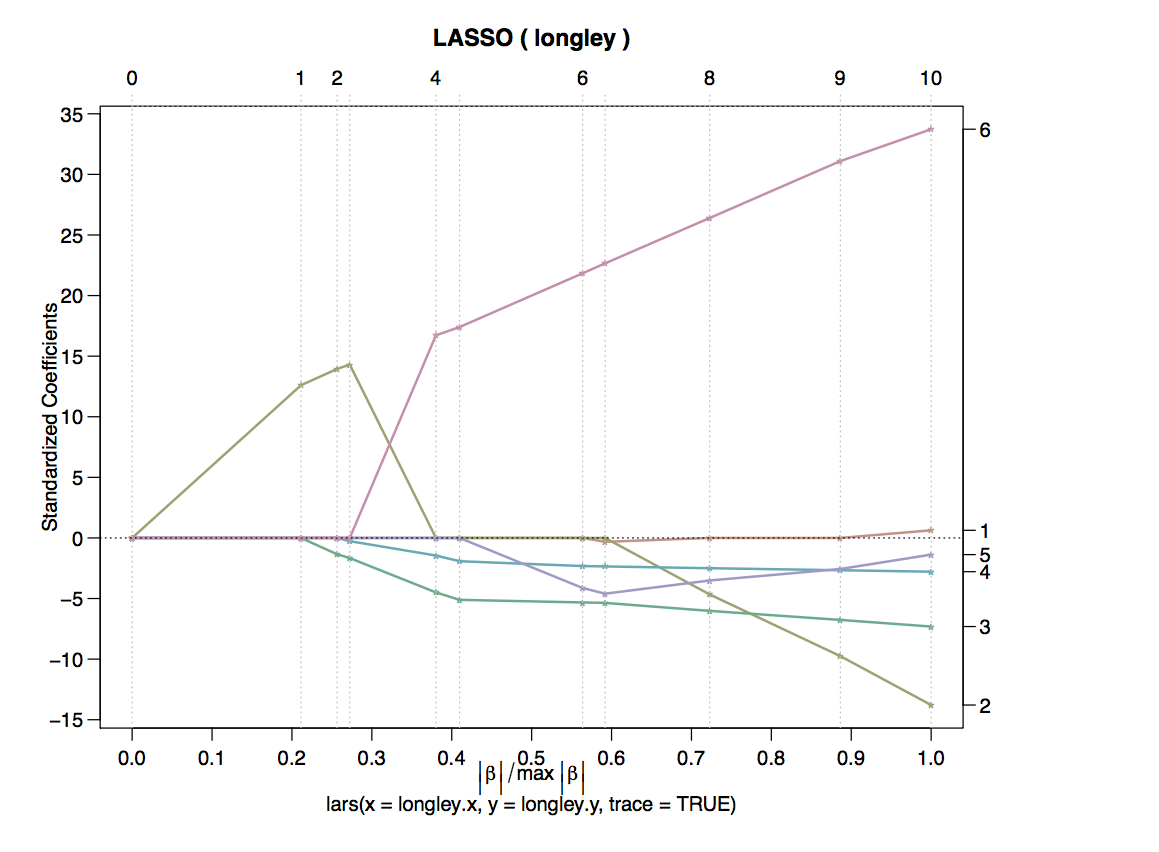
\includegraphics[width=16.1in]{figures/lasso_trace}

The above plot shows the Lasso traces for six coefficients. On the
x-axis we don't have lamda, but the norm of the Beta vector.
\(max |\beta|\) corresponds to the OLS solution with \(\lambda = 0\)
since for any other value of \(\lambda\), the norm is smaller. Hence,
\(x = 1\) corresponds to the OLS solution. On the other hand, \(x = 0\)
corresponds to \(\lambda = \infty\), since \(\|\beta\|\) equals zero. In
this case, all coefficients are zero obviously.

Note that both Lasso and Ridge regression have \emph{worse} in-sample
performance than OLS, since the coefficients are biased. However, the
out-of-sample performance is better since the bias variance trade-off is
optimized.

\section{Extensions}\label{extensions}

\subsection{Elastic Net}\label{elastic-net}

The elastic net combines the penalties used in ridge regression and
lasso.
\[ \hat{\beta} =  \|Y- X\beta\|^2 \;\; \text{subject to}\; (1 - \alpha) \|\beta\|_1 + \alpha \|\beta\|^2 <t\]
The lasso penalty \((1 - \alpha) \|\beta\|_1 + \alpha \|\beta\|^2\) is a
sum of a structky convex function and a convex function and hence
strictly convex.

\subsection{Adaptive Lasso}\label{adaptive-lasso}

The idea is to use a different weight for each coefficient in the
penalty term:
\[ \hat{\beta} =  \arg\min\|Y- X\beta\|^2 \;\; + \lambda \sum\limits_{j = 1}^p w_j|\beta_j|\]
The idea is now to use consistent esitimates for all coefficients,
e.g.~through least squares. Then, do a lasso and set
\(w_j = \frac{1}{\hat{\beta_j}}\). This means that we now penalize small
coefficients more, so they get shrunken to zero more quickly, whereas
large coefficients (which are clearly non-zero) are given a low weight
so their bias after the shrinkage is small

\subsection{Relaxed Lasso}\label{relaxed-lasso}

The relaxed lasso is also based on the idea of doing variable shrinkage
isolated from variable selection. Hence, the idea is doing a lasso first
to obtain the relevant variables. Then, a combination between lasso and
OLS is used to obtain the final model

\[\hat{\beta}^{\lambda, \phi} = \arg\min\limits_{\beta} \sum\limits_{i = 1}^n(yi - 
\sum\limits_{j \in \mathcal{M}_\lambda} \beta_j x_{i, j})^2 + 
\lambda \phi \sum\limits_{j = 1}^p|\beta_j|\]

For \(\phi = 0\), the final estimates are just the OLS estimates with
\(\mathcal{M}_\lambda\), \(\phi = 1\) just reproduces the lasso that was
used for variable selection.

\subsection{(Sparse) Group Lasso}\label{sparse-group-lasso}

When dealing with categorical data with \$ J\textgreater{}2\$, the
techniques introduced above have the drawback that they may select just
a few of the dummy variables to be non-zero. However, for
interpretability, we want to keep all or none of the dummies in the
model instead of selecting each variable \emph{independently}. This can
be achieved with a group lasso. We first split the design matrix into
\(L\) design matrices where each of them contains a block of \(p_l\)
predictors and all observations and it holds that
\(\sum\limits_{p = 1}^L p_l = p\). We also split the corresponding
coefficient vector \(\beta\) into pieces. Then, we group-wise scaled L2
penalties.

\[ \|Y-\sum\limits_{l = 1}^L X_l\beta_l \|_2^2 + 
\lambda \sum\limits_{l = 1}^L \sqrt{p_l} \|\beta_l\|_2\] Each continuous
predictor forms its own group, categorical predictors are put in one
group. Note that for \(L = p\), the problem reduces to a lasso\\
although we have an L2-penalty. This is because the L2 norm and the L1
norm of a scalar concide, or mathematically speaking
\(\||s\|_2 = \sqrt{s^2} = |s| = \|s\|_1\). This acts like a lasso on the
group level, i.e.~it sets all coefficients of a group to zero - or none
of them.

There is an extension called \emph{sparse group lasso} which can bring
sprasity within a group. This is not helpful for dummy variables, but
for situations where you have predictors that form a group since they
are highly correlated or otherwise connected. It also applies the idea
of an elastic net penalty to the group lasso. The formula is

\[ \|Y-\sum\limits_{l = 1}^L X_l\beta_l \|_2^2 + 
\lambda_1 \sum\limits_{l = 1}^L \sqrt{p_l} \|\beta_l\|_2 + 
\lambda_2 \|\beta_l \|_1\]

\subsection{Oracle Properties}\label{oracle-properties}

The adaptive lasso (unlike all other lasso-related techniques presented
here posseses so-called oracle properties). Consider the set
\$\mathcal{M}, which contains the all non-zero perdictor variabiables
from a large number of available predictors.
\[ \mathcal{M} = \{j \in \{1, ..., p\}; \; \beta_j \neq 0\}\] The set
\(\mathcal{M}_\lambda\) contains all predictors that were estimated to
be non-zero via a Lasso estimate
\[ \mathcal{M}_\lambda = \{j \in \{1, ..., p\}; \; \hat{\beta}_j \neq 0\}\]
An estimator has oracle properties if
\[ \mathcal{M}_\lambda =\mathcal{M} \; \text{for} \; n \rightarrow \infty\]
Lasso typically produces too large of non-zero predictors, but all
non-zero predictors are in that set, that is
\[  \mathcal{M}_{\lambda}^{Lasso} \supset \mathcal{M} \]

\chapter{Bagging and Boosting}\label{bagging-and-boosting}

Bagging stands for bootstrapping aggregating and

\section{Bagging}\label{bagging}

Bagging works as follows: Consider a base procedure
\[ \hat{g}(\cdot): \mathbb{R}^p \rightarrow \mathbb{R}\]

\begin{enumerate}
\def\labelenumi{\arabic{enumi}.}
\tightlist
\item
  Draw a bootstrap sample \((Y_1^*, X_1^*), ..., (Y_1^*, X_n^*)\) and
  compute the bootstrap estimator \(\hat{g(\cdot)}^*\).
\item
  Repeat the above step \(B\) times yielding
  \(\hat{g}(\cdot)^{*1}, ..., \hat{g}(\cdot)^{*B}\) bootstrap estimators
\item
  Average the estimates to construct the bagged estimator:
  \[ \hat{g}_{Bag}(x) = n^{-1} \sum\limits_{i = 1}^B\hat{g}(\cdot)^{*i}\]
  Then, \(\hat{g}(\cdot)\) is nothing else than an approximation of the
  bootstrap expectation.
  \[\hat{g}(\cdot) \approx \mathbb{E}^*[g(x)^{*}]\] Note that the novel
  point is that we now use this approximation as an estimate of
  \(g(\cdot)\). However,

  \begin{equation}
     \begin{split}
     \hat{g}(\cdot)_{Bag} & = \hat{g}(\cdot) + \mathbb{E}^*[g(x)^{*}] - \hat{g}(\cdot) \\
     & = \hat{g}(\cdot) + \text{bootstrap bias estimate}
     \end{split}
     \end{equation}
\end{enumerate}

Instead of subtracting the bootstrap bias estimate, we are adding it!
However, for trees for example, bagging reduces the variance of the
estimate so much that the bias increase will not be strong enough to
push the mean square error up. Let us consider a one-dimensional
example.

The variance of an indicator function (which is a Bernoulli experiment)
is given by
\[ Var(1_{X>d}) = \mathbb{P}(X > d)(1 - (\mathbb{P}(X > d))\] If we
assume \(X \sim N(0, 1)\) and \(d = 0\),
\(\mathbb{P}(X > d) = 1 - \mathbb{P}(X<d) = 0.5\), so the above quantity
is \(1/4\). For bagged trees, it turns out that the estimator is a
product of probit functions \(\phi(d-X)\). Since it holds that
\[ \text{if}\;\; X \sim F, \;\;F(X) \sim U\] the variance of random
forest is \[Var(\phi(d-X)) = Var(U) = 1/12\] So the variance was reduced
by a factor of 3.

\section{Subagging}\label{subagging}

Subagging stands for sub-sampling and aggregation. It is different from
bagging in that instead of drawing bootstrap samples of size \(n\), we
only draw samples of size \(m < n\), that is
\((X_1^*, Y_1^*), ..., (X_m^*, Y_m^*)\) but \textbf{without
replacement}. It can be shown that for some situations, subagging with
\(m = n/2\) is equivalent to bagging, hence, subagging is a cheap
version of bagging.

Bagging (and subagging) have one drawback which is the lack of
interpretability. In the script, there is a comparison between MARS and
trees. Both subagging and bagging helps for trees, but does not help for
MARS. How come? Remember that fitted values of trees are piece-wise
constant. Bagging makes them smoother (and hence more like MARS). MARS
yield a piece-wise linear function by nature. Trees have a high variance
and hence the bias-variance trade-off can be optimized with bagging.
MARS don't have such a high variance, hence, optimization is not
possible to the same extend.

\section{\texorpdfstring{\(L_2\)-Boosting}{L\_2-Boosting}}\label{l_2-boosting}

We saw bagging was a variance reduction technique. Boosting is a bias
reduction technique. As with bagging there is a base estimator
\(\hat{g}(\cdot)\). Then, you basically refit it to the residuals to
reduce them many times. The concrete implementation is:

\begin{itemize}
\item
  Fit an estimator to the data and compute the residuals
  \[U_i = Y_i - \nu\hat{g}_1(x_i)\] where \$\nu \textless{} 1 \$ is a
  tuning parameter. The smaller \(\nu\), the more \emph{explainable}
  residuals you leave for suceeding estimators. Denote
  \(\hat{f}_1(x) = \nu g_1(x)\)
\item
  For m = 2, 3, \ldots{}, M: Fit the residuals to the data, i.e
  \[ (U_i, X_i) \rightarrow \hat{g}(x)\] Set
  \[ \hat{f}_m(x) = \hat{f}_{m-1}(x) + \nu \hat{g}_m(x)\] Compute the
  current residuals: \[U_i = Y_i - \hat{f}_m(x)\]
\end{itemize}

A small \(\nu\) can be interpreted as follows: You go into the right
direction, but you do that slowly and you allow yourself to be corrected
later.

Boosting can be useful in the context of thinning-out with trees, where
you don't have enough observations in the terminal nodes to continue.
Boosting then comes up with a more complex solution by taking
\emph{linear combinations} of trees. For classificcation trees, you can
also extend the tree by taking

Boosting can also be used for varible selection. For example, let
\(\hat{g}\) be a GAM with one predictor. Then, for each variable fit
such a gam and set
\(f_1(x) = arg\min\limits_{\hat{g}_j(x) \; j =\{1, ..., p\}}\|Y - \hat{g}_j(x)\|\),
i.e.~take the the additive model that had the smallest residual sum of
squares. Then, use the \emph{adjusted} residuals from it and fit another
\(p\) GAMs and select again the gam with the smallest RSS.

\section{Some unfinished stuff}\label{some-unfinished-stuff}

Let's consider a simple one-dimensional example. If you have a cut-off
at \(d\) (so for example for classification, \(X > d\) is classified as
\(1\), \(X < d\) as \(0\)) and you take the mean over many bootstrap
samples (which you do with random forests, where each tree has a
potentially different \(d\)), with \(n \rightarrow \infty\) you get a
smooth function (probably some form of a transformed binomial that is
asymptotically normal)

\begin{Shaded}
\begin{Highlighting}[]
\NormalTok{one_mean <-}\StringTok{ }\NormalTok{function(}\DataTypeTok{d =} \DecValTok{0}\NormalTok{, ...) \{}
  \NormalTok{x <-}\StringTok{ }\KeywordTok{rnorm}\NormalTok{(...)}
  \NormalTok{x_boolean <-}\StringTok{ }\NormalTok{x >}\StringTok{ }\NormalTok{d}
  \KeywordTok{mean}\NormalTok{(x_boolean)}
\NormalTok{\}}

\NormalTok{mean_sim <-}\StringTok{ }\KeywordTok{rerun}\NormalTok{(}\DecValTok{1000}\NormalTok{, }\KeywordTok{one_mean}\NormalTok{(}\DataTypeTok{n =} \DecValTok{200}\NormalTok{)) %>%}
\StringTok{  }\KeywordTok{flatten_dbl}\NormalTok{()}

\KeywordTok{ggplot}\NormalTok{(}\KeywordTok{data_frame}\NormalTok{(}\DataTypeTok{mean =} \NormalTok{mean_sim), }\KeywordTok{aes}\NormalTok{(}\DataTypeTok{x =} \NormalTok{mean)) +}
\StringTok{  }\KeywordTok{stat_ecdf}\NormalTok{(}\DataTypeTok{geom =} \StringTok{"step"}\NormalTok{)}
\end{Highlighting}
\end{Shaded}

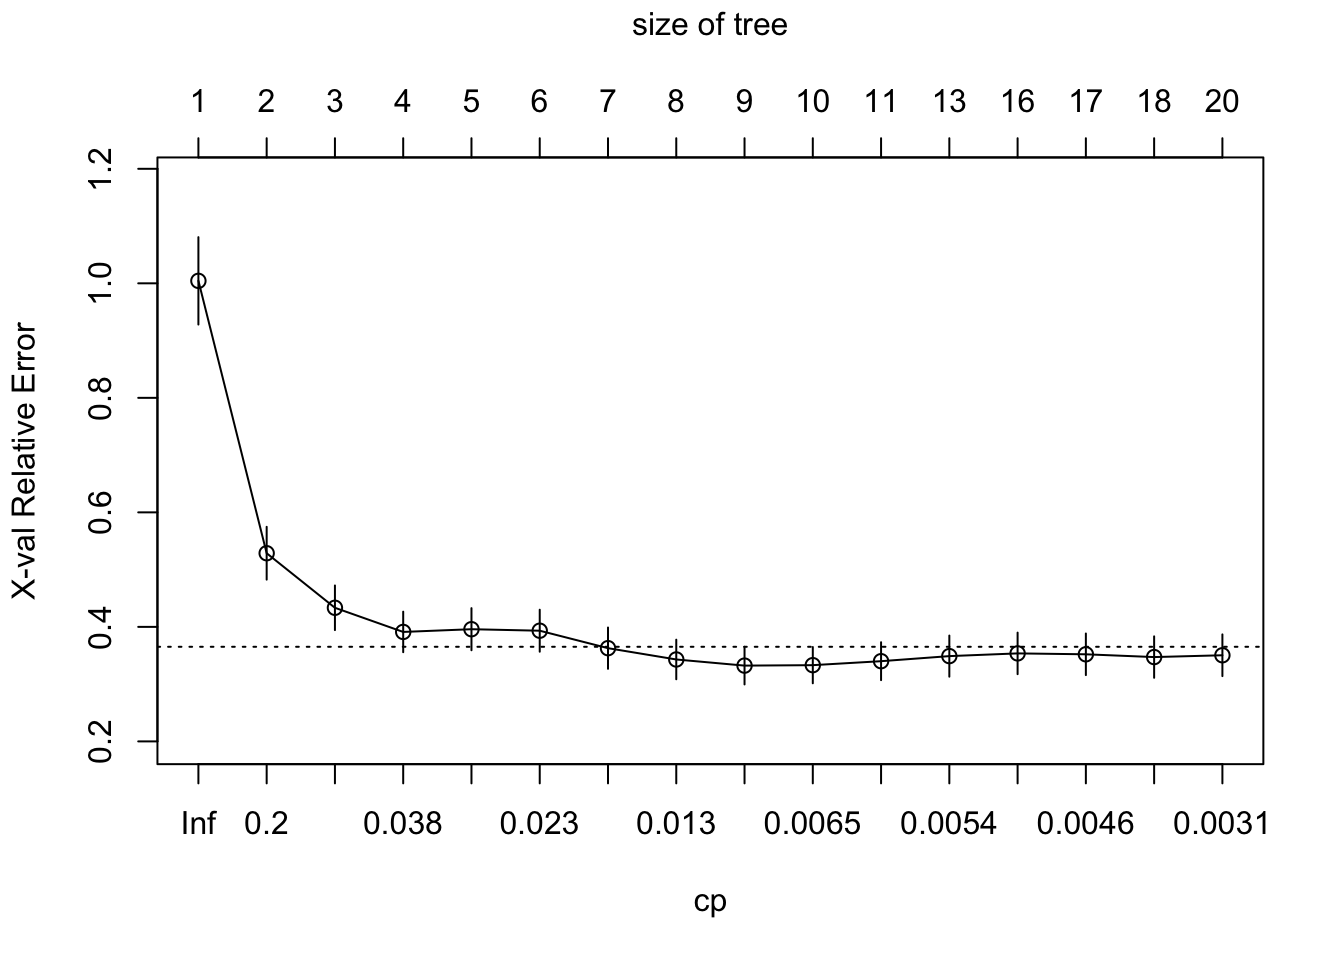
\includegraphics{comp_stats_summary_files/figure-latex/unnamed-chunk-36-1.pdf}

Here you can see that if \(x \sim F\), \(F(X) \sim Unif\).

\begin{Shaded}
\begin{Highlighting}[]
\NormalTok{x <-}\StringTok{ }\KeywordTok{rnorm}\NormalTok{(}\DecValTok{1000}\NormalTok{)}
\KeywordTok{plot.ecdf}\NormalTok{(x)}
\end{Highlighting}
\end{Shaded}

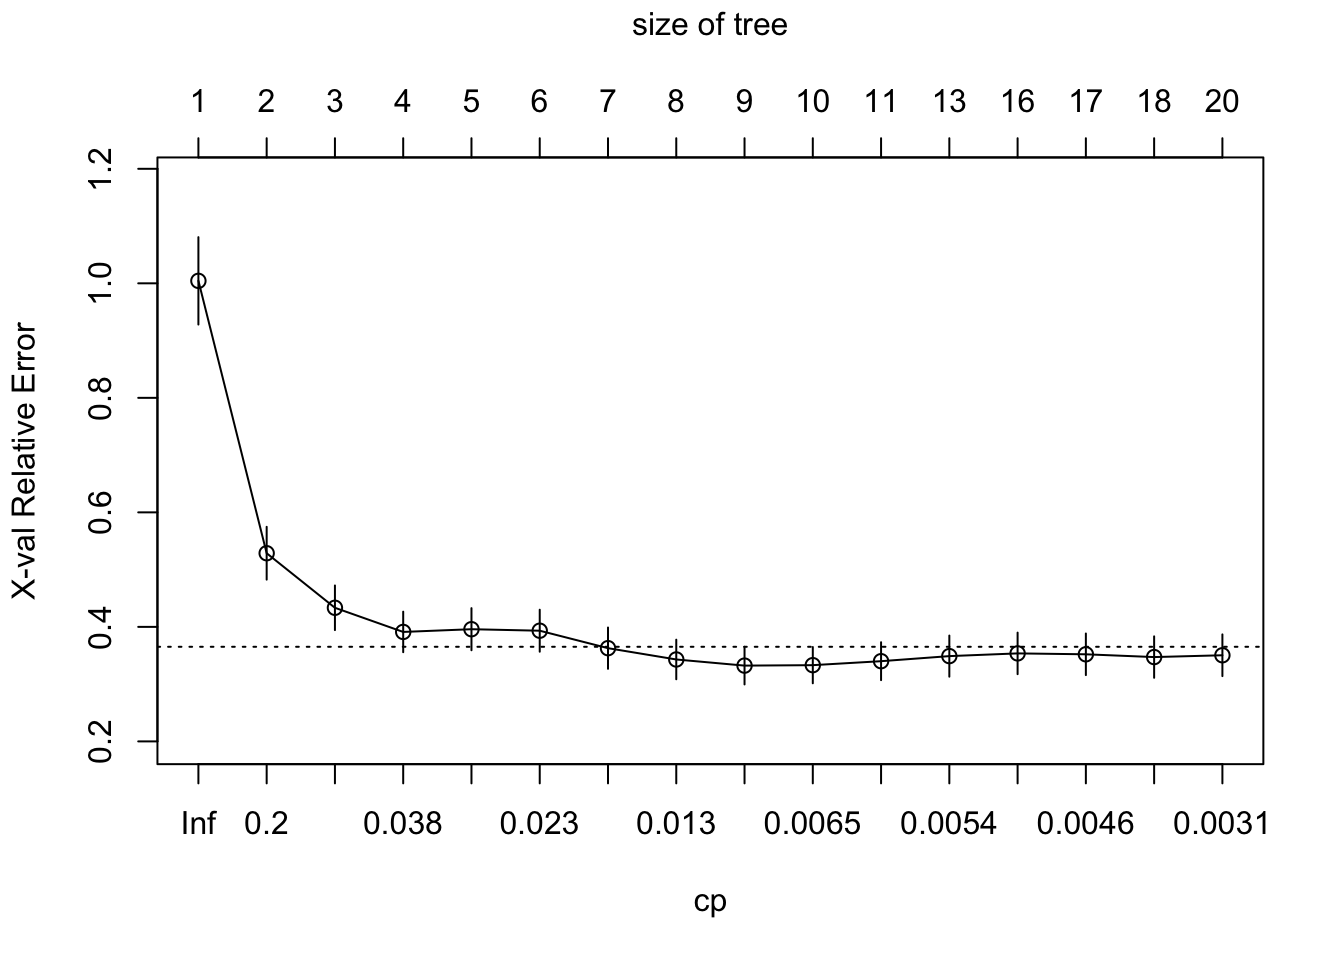
\includegraphics{comp_stats_summary_files/figure-latex/unnamed-chunk-37-1.pdf}

\begin{Shaded}
\begin{Highlighting}[]
\NormalTok{y <-}\StringTok{ }\KeywordTok{pnorm}\NormalTok{(x)}
\KeywordTok{plot.ecdf}\NormalTok{(y)}
\end{Highlighting}
\end{Shaded}

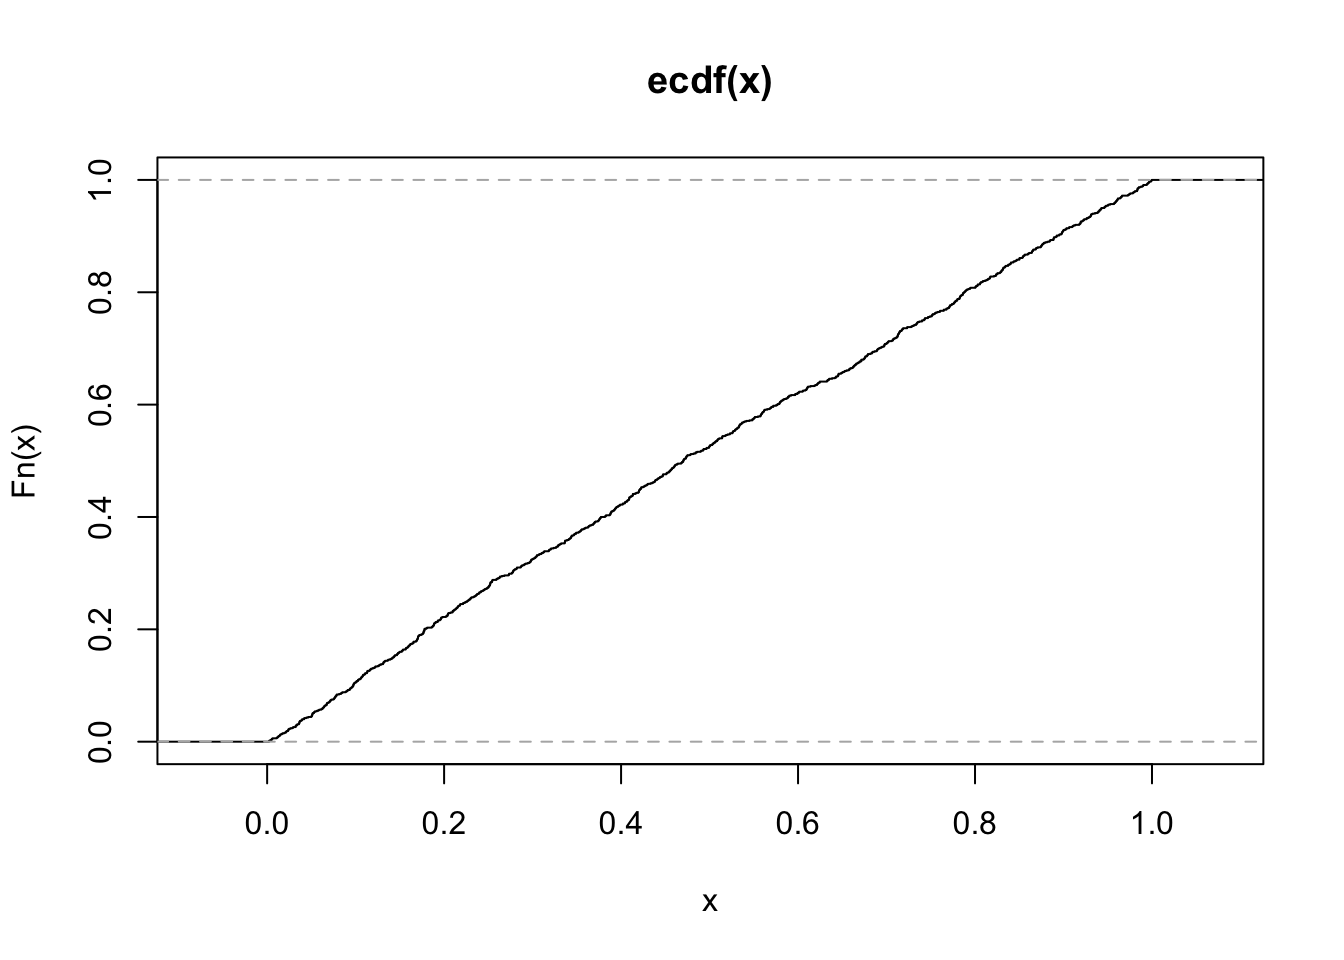
\includegraphics{comp_stats_summary_files/figure-latex/unnamed-chunk-37-2.pdf}

\chapter{Introduction}\label{intro}

You can label chapter and section titles using \texttt{\{\#label\}}
after them, e.g., we can reference Chapter \ref{intro}. If you do not
manually label them, there will be automatic labels anyway, e.g.,
Chapter \ref{methods}.

Figures and tables with captions will be placed in \texttt{figure} and
\texttt{table} environments, respectively.

\begin{Shaded}
\begin{Highlighting}[]
\KeywordTok{par}\NormalTok{(}\DataTypeTok{mar =} \KeywordTok{c}\NormalTok{(}\DecValTok{4}\NormalTok{, }\DecValTok{4}\NormalTok{, .}\DecValTok{1}\NormalTok{, .}\DecValTok{1}\NormalTok{))}
\KeywordTok{plot}\NormalTok{(pressure, }\DataTypeTok{type =} \StringTok{'b'}\NormalTok{, }\DataTypeTok{pch =} \DecValTok{19}\NormalTok{)}
\end{Highlighting}
\end{Shaded}

\begin{figure}

{\centering 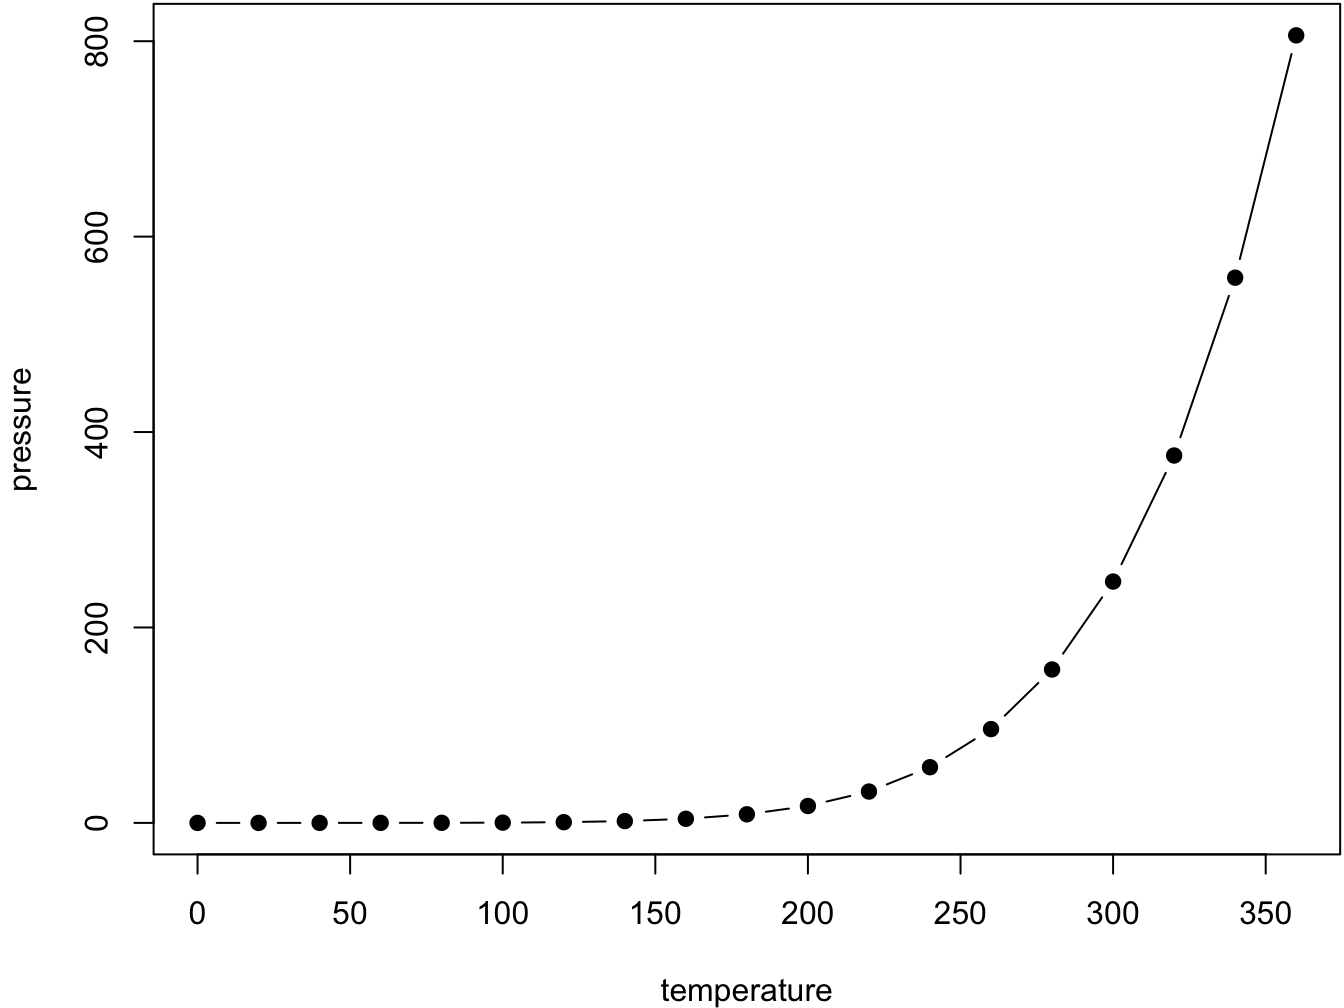
\includegraphics[width=0.8\linewidth]{comp_stats_summary_files/figure-latex/nice-fig-1} 

}

\caption{Here is a nice figure!}\label{fig:nice-fig}
\end{figure}

Reference a figure by its code chunk label with the \texttt{fig:}
prefix, e.g., see Figure \ref{fig:nice-fig}. Similarly, you can
reference tables generated from \texttt{knitr::kable()}, e.g., see Table
\ref{tab:nice-tab}.

\begin{Shaded}
\begin{Highlighting}[]
\NormalTok{knitr::}\KeywordTok{kable}\NormalTok{(}
  \KeywordTok{head}\NormalTok{(iris, }\DecValTok{20}\NormalTok{), }\DataTypeTok{caption =} \StringTok{'Here is a nice table!'}\NormalTok{,}
  \DataTypeTok{booktabs =} \OtherTok{TRUE}
\NormalTok{)}
\end{Highlighting}
\end{Shaded}

\begin{table}

\caption{\label{tab:nice-tab}Here is a nice table!}
\centering
\begin{tabular}[t]{rrrrl}
\toprule
Sepal.Length & Sepal.Width & Petal.Length & Petal.Width & Species\\
\midrule
5.1 & 3.5 & 1.4 & 0.2 & setosa\\
4.9 & 3.0 & 1.4 & 0.2 & setosa\\
4.7 & 3.2 & 1.3 & 0.2 & setosa\\
4.6 & 3.1 & 1.5 & 0.2 & setosa\\
5.0 & 3.6 & 1.4 & 0.2 & setosa\\
\addlinespace
5.4 & 3.9 & 1.7 & 0.4 & setosa\\
4.6 & 3.4 & 1.4 & 0.3 & setosa\\
5.0 & 3.4 & 1.5 & 0.2 & setosa\\
4.4 & 2.9 & 1.4 & 0.2 & setosa\\
4.9 & 3.1 & 1.5 & 0.1 & setosa\\
\addlinespace
5.4 & 3.7 & 1.5 & 0.2 & setosa\\
4.8 & 3.4 & 1.6 & 0.2 & setosa\\
4.8 & 3.0 & 1.4 & 0.1 & setosa\\
4.3 & 3.0 & 1.1 & 0.1 & setosa\\
5.8 & 4.0 & 1.2 & 0.2 & setosa\\
\addlinespace
5.7 & 4.4 & 1.5 & 0.4 & setosa\\
5.4 & 3.9 & 1.3 & 0.4 & setosa\\
5.1 & 3.5 & 1.4 & 0.3 & setosa\\
5.7 & 3.8 & 1.7 & 0.3 & setosa\\
5.1 & 3.8 & 1.5 & 0.3 & setosa\\
\bottomrule
\end{tabular}
\end{table}

You can write citations, too. For example, we are using the
\textbf{bookdown} package {[}@R-bookdown{]} in this sample book, which
was built on top of R Markdown and \textbf{knitr} {[}@xie2015{]}.


\end{document}
